\newpage
\section{Application of LC and APC models to German cancer data}
\textcolor{myDarkGreen}{Innledning - presenter hva som skal gjøres:
\begin{itemize}
    \item Prediksjon med APC og LC modeller
    \item Først univariate, så multivariate
\end{itemize}
}
In the second part of our investigation, we apply the Lee-Carter methods to real data and use \inlabru to make inference. We compare the results to the application of APC-models on the same data sets, also using \inlabru. Note that in the case of the APC model, inference with \inlabru will yield the same results as inference using only \inla. Since the random effects in the APC model are not uniquely identifible, we compare the two models by their predictive abilities. We test both univariate and multivariate versions of the Lee-Carter and APC models (the latter with sex as a covariate), and we begin with the univariate case. 
\subsection{German cancer data}
\label{sec:GermanCancerData}
\textcolor{myDarkGreen}{
Presenter datasettene. Si noe om hvor de kommer fra, hvordan de opprinnelig er aggregert og hvordan du har aggregert dem. Plott dataen aggregert over cohort, alder og period. Fortell hvordan du indekserer alder, cohort og period og si at denne indekseringen vil benyttes for alle modellene. Legg vekt på at kohort-indeksen skiller seg fra synthetic-data stadiet siden du har forskjellige intervaller. Referer til Andrea sin metode å løse det på. 
}
We use data of mortality for lung and stomach cancer in Germany in the years 1999-2016, obtained from \texcite{cancerData}. In these data sets, the observed mortality for the two cancer types are given by the number of cases for male and females, for each year, for five-year age intervals. The exception is for the ages above 85 year, which are collected in a single group. For the univariate part of our analysis, we add the male and female cases to obtain the total mortality for male and female. We find data for the total German population for the corresponding years and ages at \texcite{germanPopulation}. This population data contains observations for age groups of one year, and we aggregate this data to the same five-year age groups as for the cancer data. We then find the mortality rates for each cancer type, for each year, age group and sex by dividing the cases of mortality by the total population for each observation. 

When formatting the data sets, it is easier to begin the indexing of age groups, period and cohorts at 0 rather than 1, so we update the indexing scheme accordingly:
\begin{itemize}
    \item The age indices $x$ are now $x = 0,\ldots,X$.
    \item The period indices $t$ are now $t = 0, \ldots, T$.
    \item The cohort indices are now given by $k = 5(X - x) + t$, $K = 5X + T$.
\end{itemize}

A summary of the data sets are presented in Figures \ref{fig:data-total} and \ref{fig:data-age-rate}. Figure \ref{fig:data-total} give a representation of the distribution of the population and the distribution of mortality cases over different age groups and years. Note that the left-most plot in Figure \ref{fig:data-total} gives a relative, but not an accurate representation, of the German population, as the people who were alive for more than one year during 1999-2016 will have been counted more than once. We observe that most cancer mortalities occur at the ages around $x = 13$, both for male and females. From the right-most part of Figure \ref{fig:data-age-rate} we observe that the observed lung cancer cases seem to increase more with time for women than for men. 

\begin{figure}
    \centering
    \begin{subfigure}[b]{.6\linewidth}
        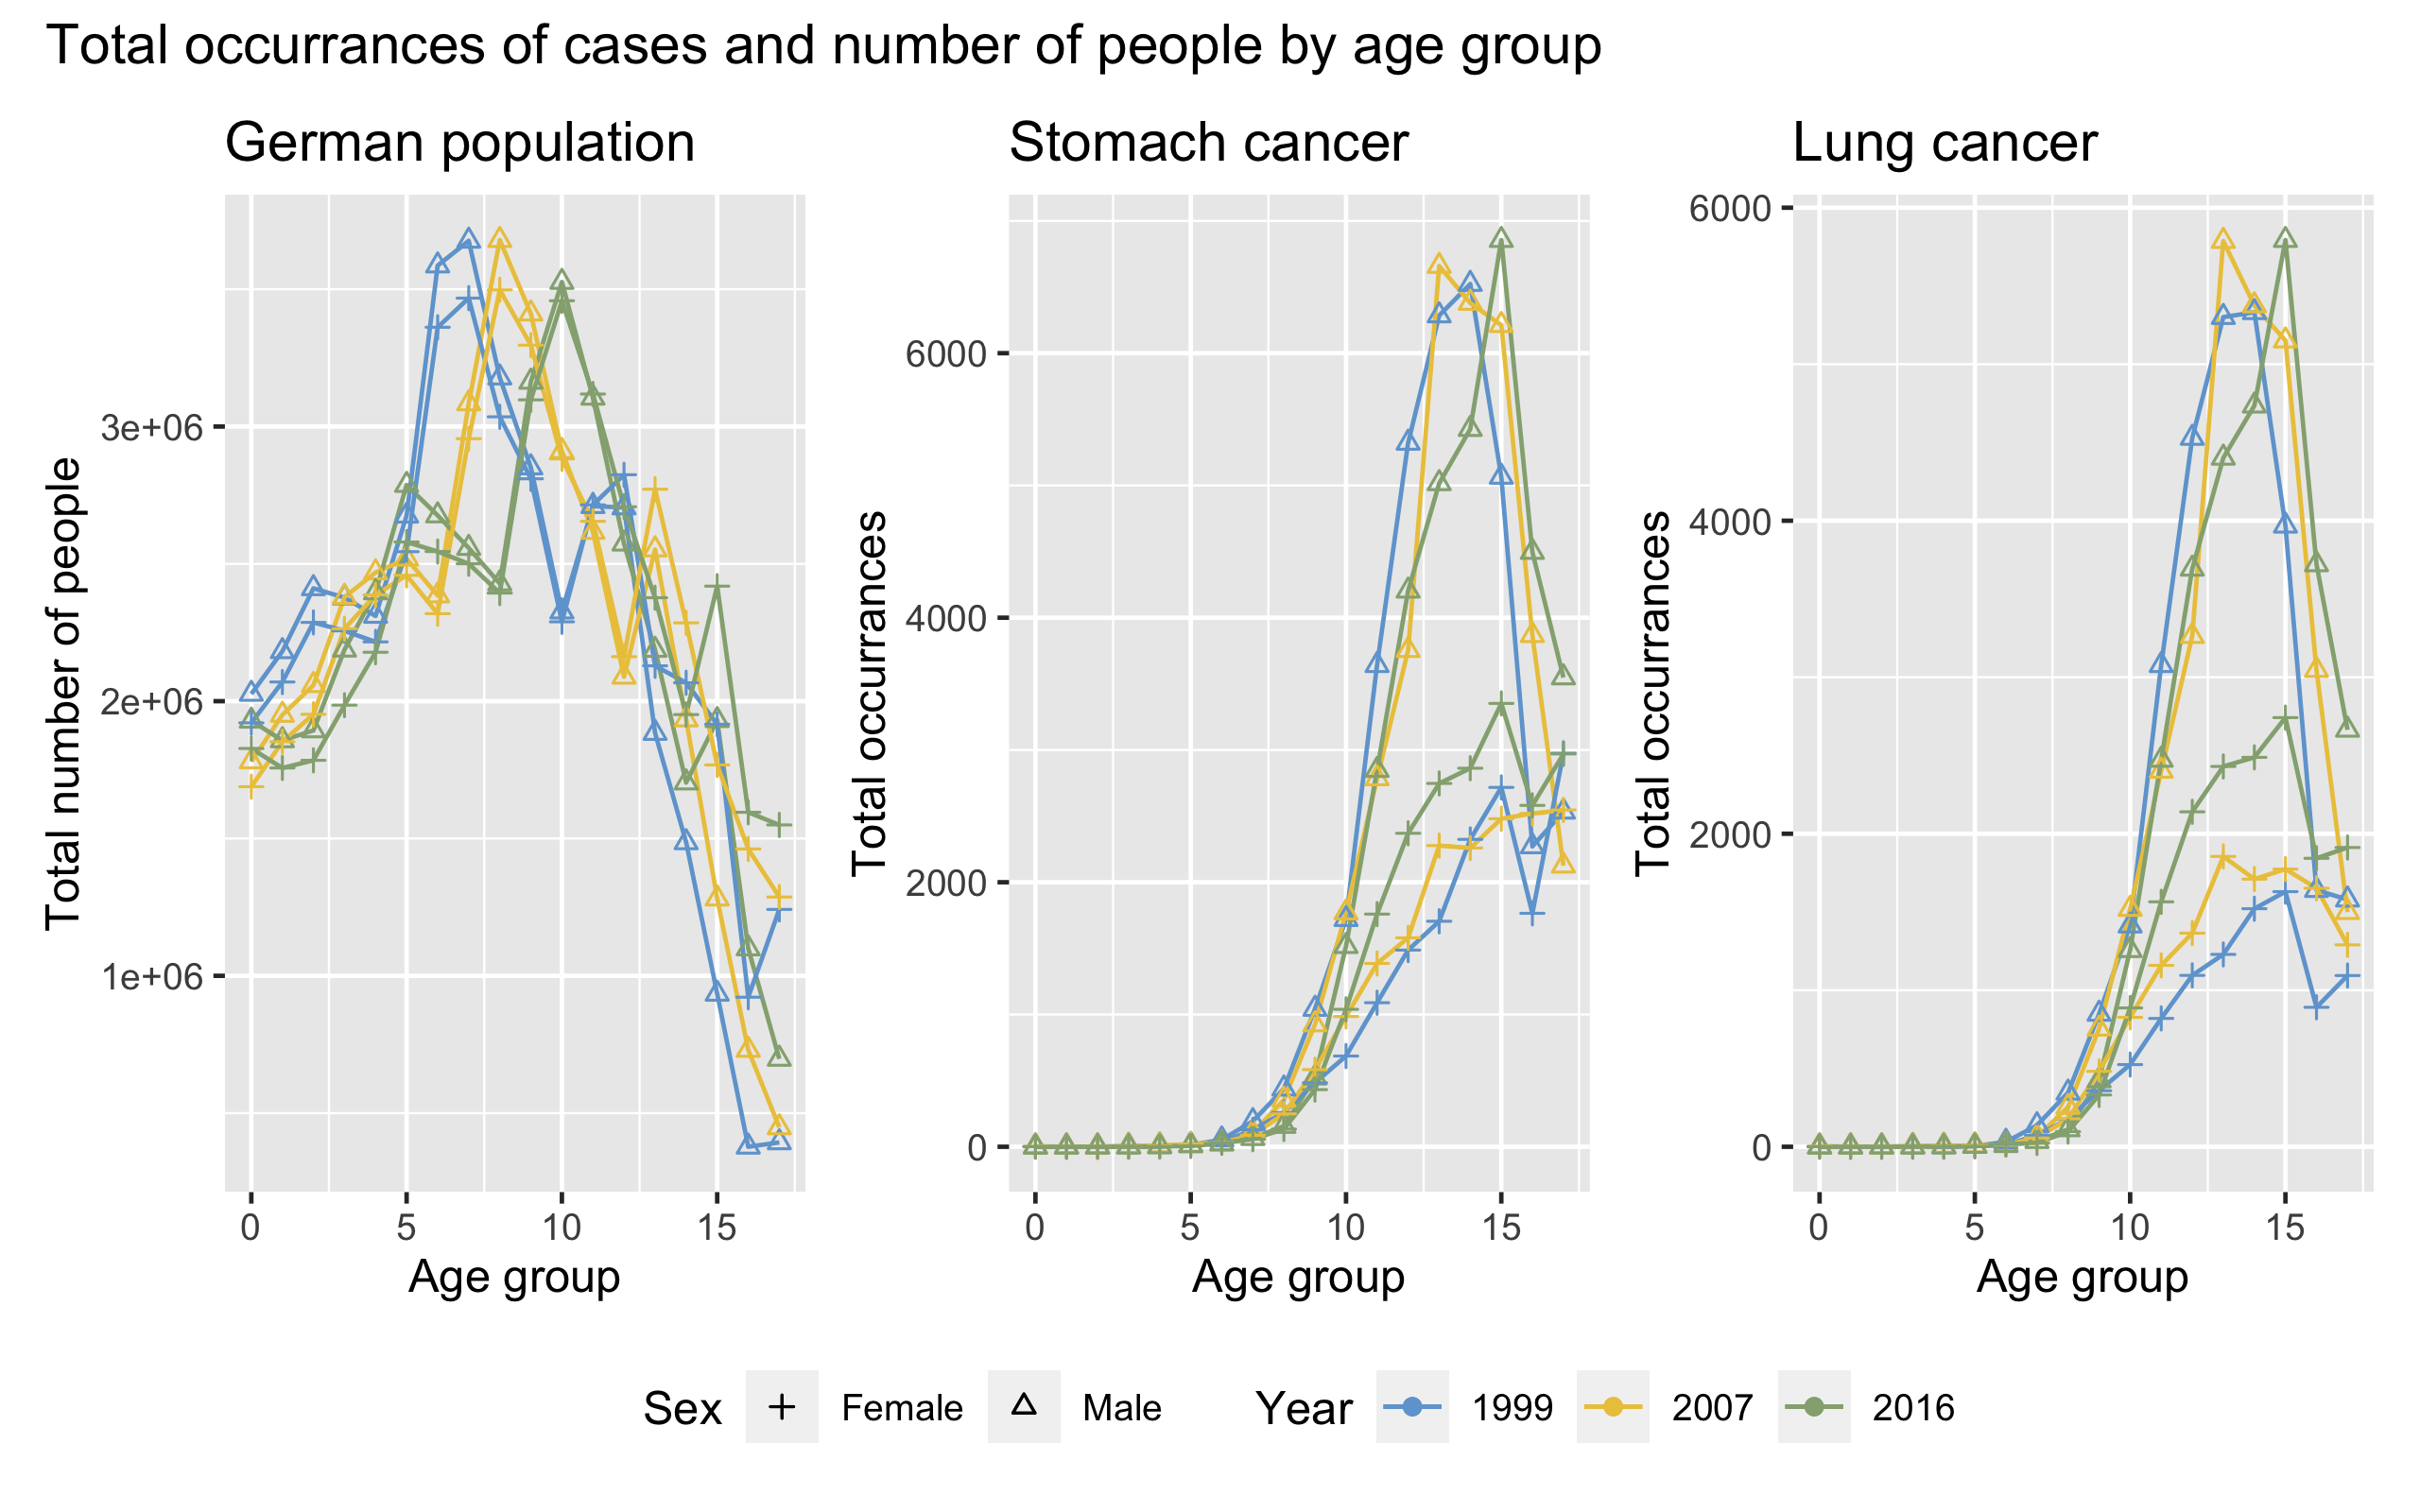
\includegraphics[width=\linewidth]{real-data/real-data-univariate/Figures/data-age-total.png}
    \end{subfigure}
    
    \begin{subfigure}[b]{.6\linewidth}
        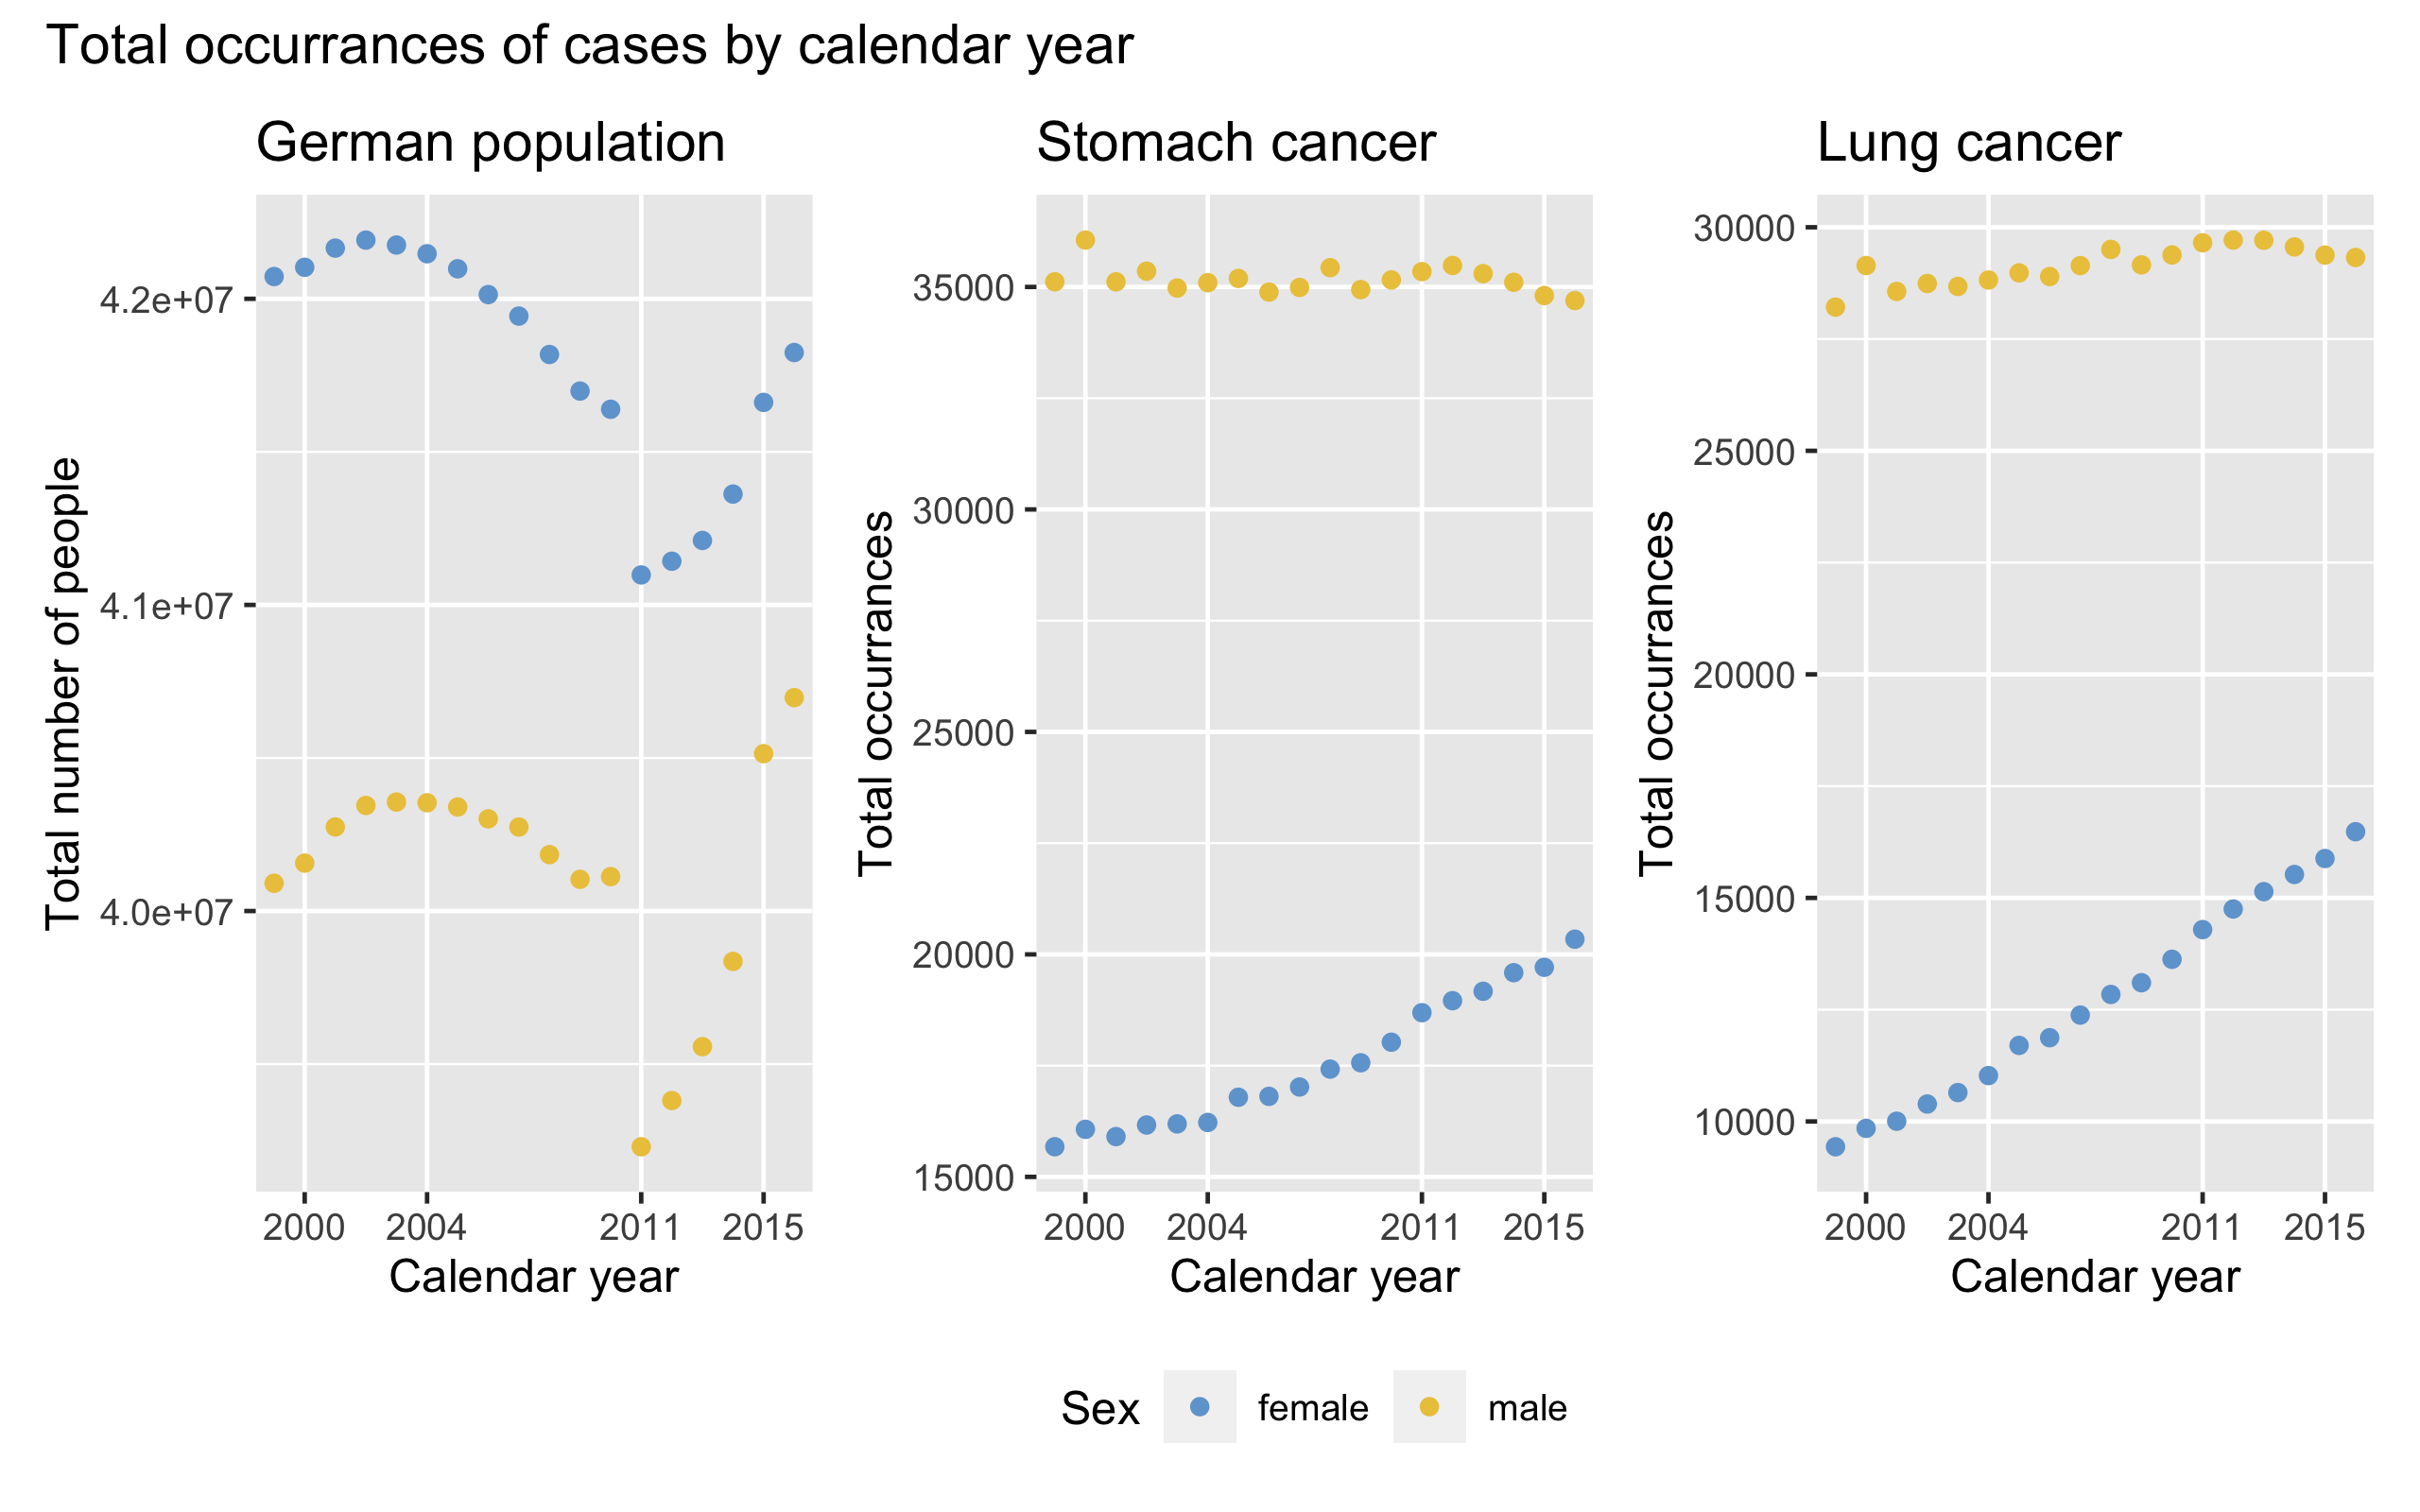
\includegraphics[width=\linewidth]{real-data/real-data-univariate/Figures/data-year-total.png}
    \end{subfigure}
    \caption{The observed population for Germany and the observed cases for lung and stomach cancer deaths. \textit{Left:} The data is summed over all years for each age group. \textit{Right:} The data is summed over all age groups for each year.}
    \label{fig:data-total}
\end{figure}

Figure \ref{fig:data-rate} present the observed mortality rates for years 1999, 2005, 2011 and 2016, for each age group and each cohort. We observe that for younger ages, the mortality rates are close to zero for both lung and stomach cancer. For the years 2005, 2011 and 2016 we see that we do not have observations for the  mortality rates for older cohorts (lower cohort index $k$). \textcolort{myDarkGreen}{What more should be said at this stage}.

\begin{figure}
    \centering
    \begin{subfigure}[b]{.45\linewidth}
        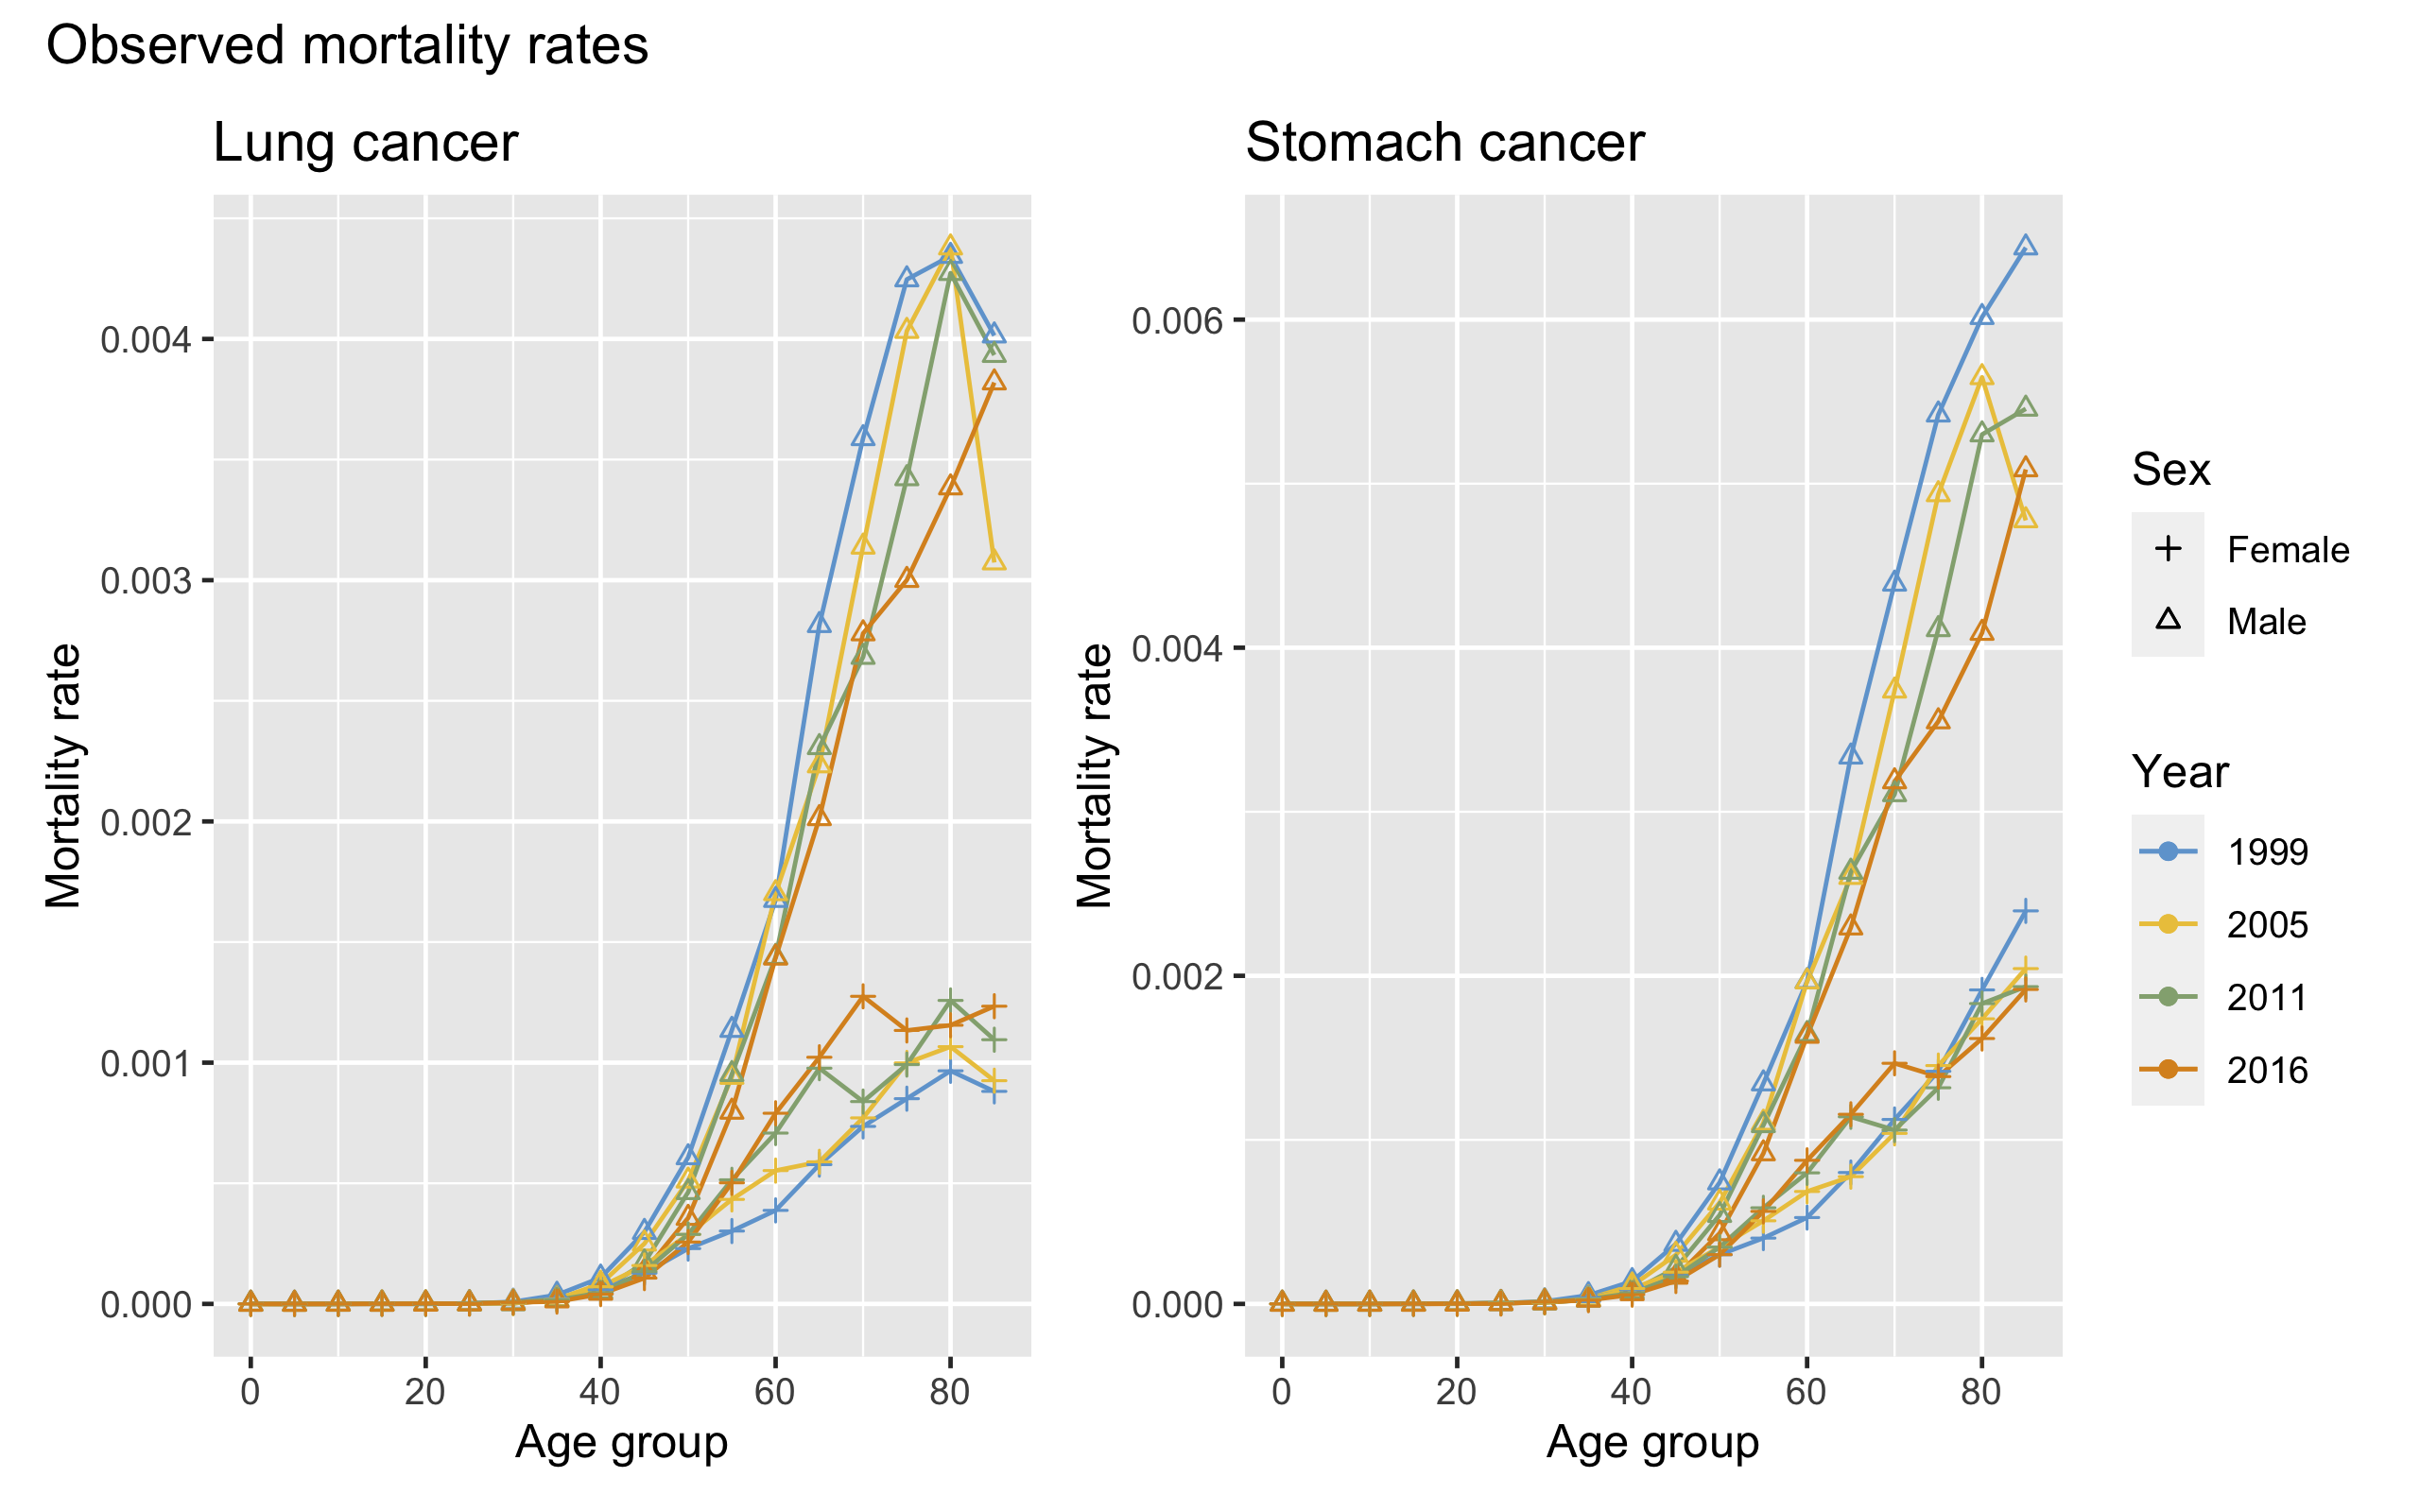
\includegraphics[width=\linewidth]{real-data/real-data-univariate/Figures/data-age-rate.png}
    \end{subfigure}
    \begin{subfigure}[b]{.45\linewidth}
        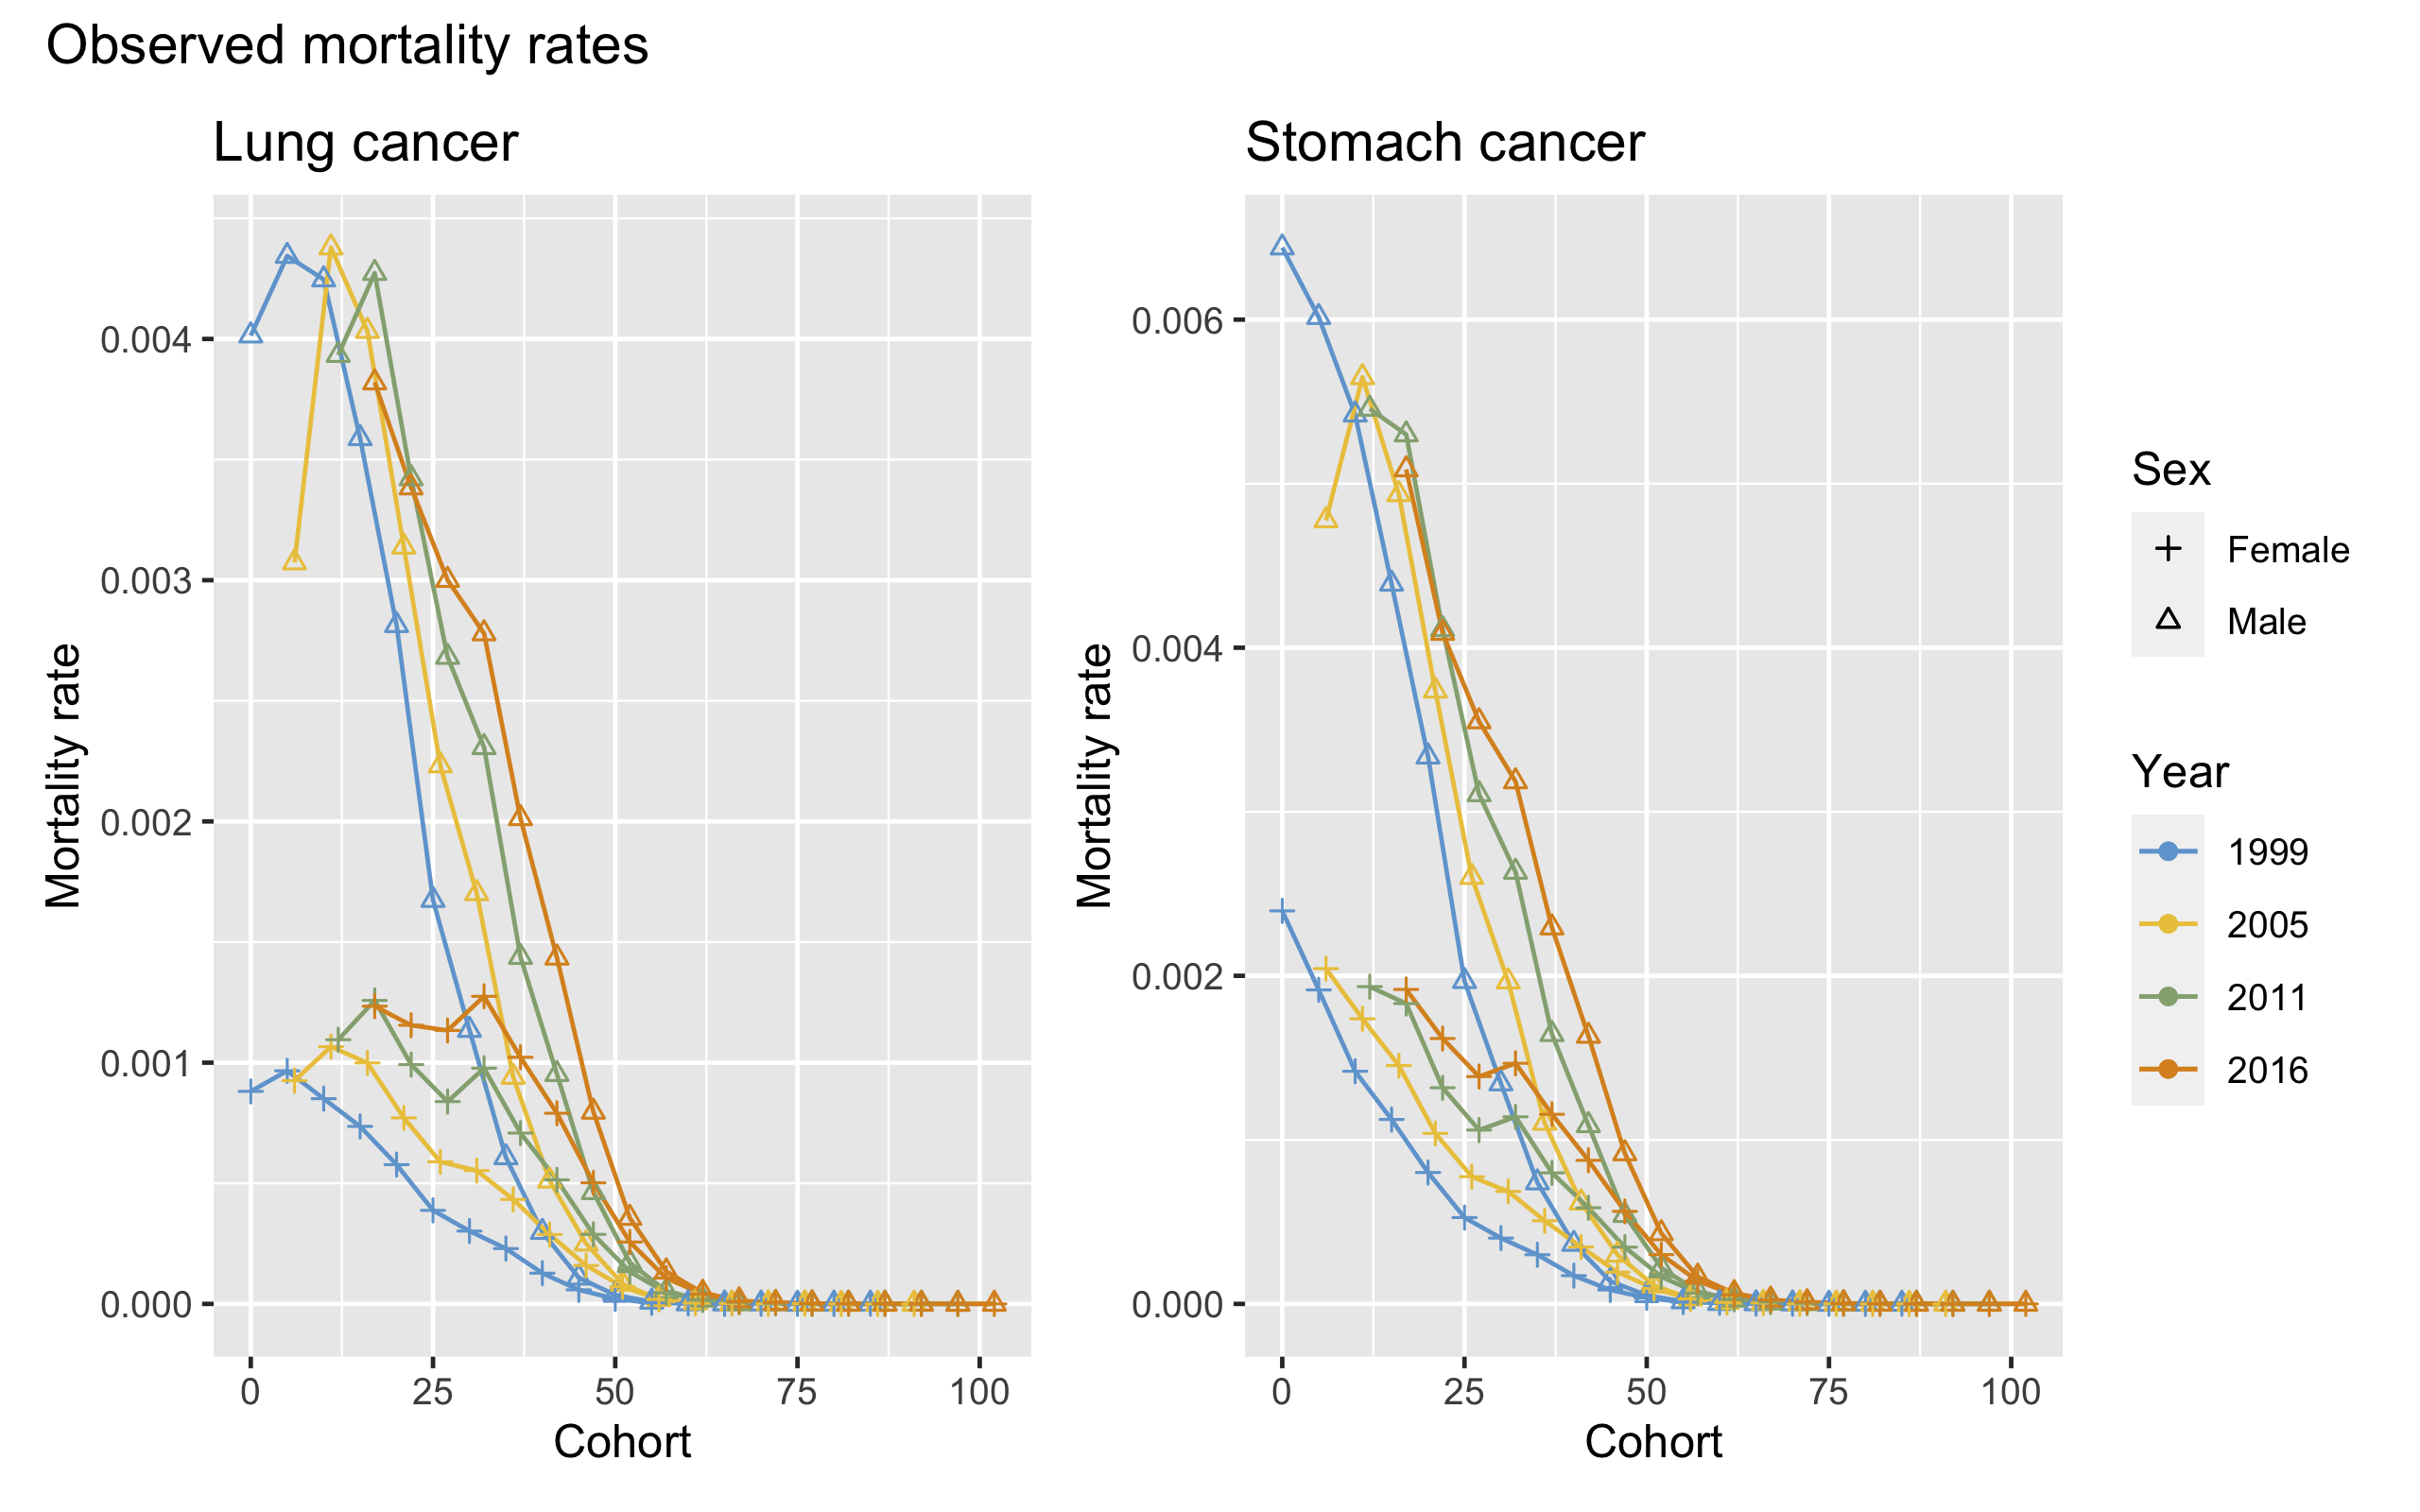
\includegraphics[width=\linewidth]{real-data/real-data-univariate/Figures/data-cohort-rate.png}
    \end{subfigure}
    \caption{The observed mortality rates for the German lung and stomach cancer data, for the years 1999, 2005, 2011 and 2016.}
    \label{fig:data-rate}
\end{figure}

\subsection{LC and LCC on full dataset}
\label{sec:LC-full-data}
To get an overview of the dataset and the performance of the LC model on these datasets, we begin by fitting the LC and the LCC model to the full datasets and compare it to plots of the data. 

\newpar Figures \ref{fig:data-by-age}, \ref{fig:data-by-year} and \ref{fig:data-by-cohort} display percent-wise deaths by lung - and stomach cancer, by age groups, years and cohorts (birth years) respectively. Figure \ref{fig:LC-full-dataset} display the random effects obtained by fitting the LC-model to the two data sets, as well as the estimated predictor. Figure \ref{fig:LCC-full-dataset} displays the results from fitting the LCC-model to the stomach cancer data set. 

\newpar From the Figure \ref{fig:LC-full-dataset} and Figure \ref{fig:LCC-full-dataset} we see that $\alphav$ is the random effect that is modeled with the highest precision for both the LC-model and the LCC-model. This indicates a clear tendency of change in the mortality rate for different age groups, with a higher mortality rate for older age groups. Figure \ref{fig:data-by-age} confirms this, as it shows a much higher mortality rate for older age groups, for both males and females. 
\newpar We observe from Figures \ref{fig:LC-full-dataset} and \ref{fig:LCC-full-dataset} that there is much higher uncertainty related to the estimation of the period effects, $\kappav$ and $\phi\cdot t$. The estimated $\kappav$ seemes in both cases to be almost insignificant, with wide confidence bounds centered around zero. The $\phi \cdot t$ effect on the other hand, does show a clear tendency of a decreasing mortality rate for higher years. [TODO: TENK GJENNOM HVORFOR PHI ER NEGATIV NÅR DU HAR EN ØKENDE TIDSTREND!! HER KAN DU JO BEGYNNE Å SPEKULERE I AT DET KANSKJE ER SMART Å HA MED EN KOHORT-EFFEKT...] We also observe a clear tendency in the cohort-effects. [OGSÅ: LEGG TIL NYE PLOTT AV EFFEKT MED LC PÅ EKTE DATA, TROR DE DU HAR NÅ KAN VÆRE UTDATERTE..]

\subsection{Prediction in the Univariate Case}
We begin by comparing prediction results for the univariate LC- and LCC-models (see Equations \ref{eq:LC-rewritten} and \ref{eq:LCC-rewritten}) to prediction results for the APC1- and APC2-models (see Section \ref{sec:BayesianInferenceAPC}).
\textcolor{myDarkGreen}{Say something of how we are now able to get a "fair" comparison - using similar priors, the same method of inference? Refer to previous papers on the same topic? }
In the comparison of the the Lee-Carter models, we include an additional version of the LCC-model, where we omit the $\beta_x\cdot \kappa_t$ term, which gives the predictor
\begin{equation}
    \eta_{x,t} = \mu + \alpha_x + \beta_x\cdot \phi \cdot t + \gamma_k + \epsilon_{x,t}.
\end{equation}
We refer to this model as the LCC-linear model, since it only has a linear period term $\phi \cdot t$. We include this model in the comparison, since we se from ... \textcolor{myDarkGreen}{You have to write this part} that the term $\kappa_t$ seem to be insignificant. Thus, we investigate if a reduced version of the model performs better. 

In order to assess the prediction quality of the different models, we divide the data sets with cancer mortality observations in half, and use the first half (years 1999-2007) to predict the mortality rates in the second half (2008-2016), given the at-risk populations from the German population data. We find the forecasts for years 2008-2016 by using \inlabru to fit the different models to the data sets, as described in Section \ref{sec:implementationInlabru}, and setting the observed deaths to missing (\texttt{NA}) for the years that we want to predict. \inlabru then automatically calculates predictions for the missing values. 
To assess the performance of the various predictions, we consider both the accuracy and the sharpness of the predictions, i.e. how close the mean predicted values are to the true mortality rates and how wide or narrow the prediction intervals are. Predictions with a higher accuracy are preferred to predictions with lower accuracy, and sharp predictions, with a narrow prediction interval, are preferred as long as the predictions are also fairly accurate. A score statistic that take all of this into consideration is the Dawid-Sebastiani Score (DSS), defined by 
\begin{equation}
    DSS = (\frac{Y_{x,t} - \mu_{x,t}}{\sigma_{x,t}})^2 + 2\cdot \log(\sigma_{x,t}).
\end{equation}
Here $Y_{x,t}$ is the observed mortality rate for age group $x$ in year $t$, $\mu_{x,t}$ is the mean of the corresponding predicted mortality rate and $\sigma_{x,t}$ is the standard deviation of the prediction \parencite{Gneiting2007}. A lower DSS score indicate a better prediction. Predictions close to the observed value give a lower score, as does a lower standard deviation (narrower prediction intervals), as long as the distance between the observed and predicted value, $\mid Y_{x,t} - \mu_{x,t} \mid$, is less than one standard deviation $\sigma$ (see \textcite{Keilman2020} for details). Following e.g. \textcite{RieblerHeldRue2012}, we use the DSS as the main scoring rule for comparison of the different prediction methods. Since the DSS is calculated for each prediction of mortality rate for age $x$ and year $t$, we take the average over all ages and periods, and use this measure, denoted MDSS, in our comparisons. In addition, to get a better impression of the qualities of the predictions, we calculate the mean squared error (MSE) and the percentage of the observations that fell within the 95\% confidence bounds of the predictions.

\newpar For younger ages, below ca. 30 years old, the mortality rates for both lung- and stomach cancer are very low, and almost at zero. All methods gives a prediction very close to zero with a very narrow prediction interval for these ages, and we are more interested in evaluating the prediction methods for mortality rates that are significantly greater than zero. Therefore, we omit the prediction values for $x \leq 5$, corresponding to ages less than 30, when calculating the score statistics. We then get a better impression of the quality of the prediction of non-zero mortality rates. 

\newpar To get sufficiently uninformative prior distributions, we set the parameters in the PC priors to
\begin{equation*}
    \mathbb{P}(1/\sqrt{\tau} > 1) = 0.05
\end{equation*}
for all precisions $\tau$ in our models. The code used to produce these results can be found in the \texttt{GitHub} repostitory, under \texttt{real-data/real-data-univariate/predict-long-term.R}. 

\begin{figure}[h!]
    \centering
    \begin{subfigure}[b]{.45\linewidth}
        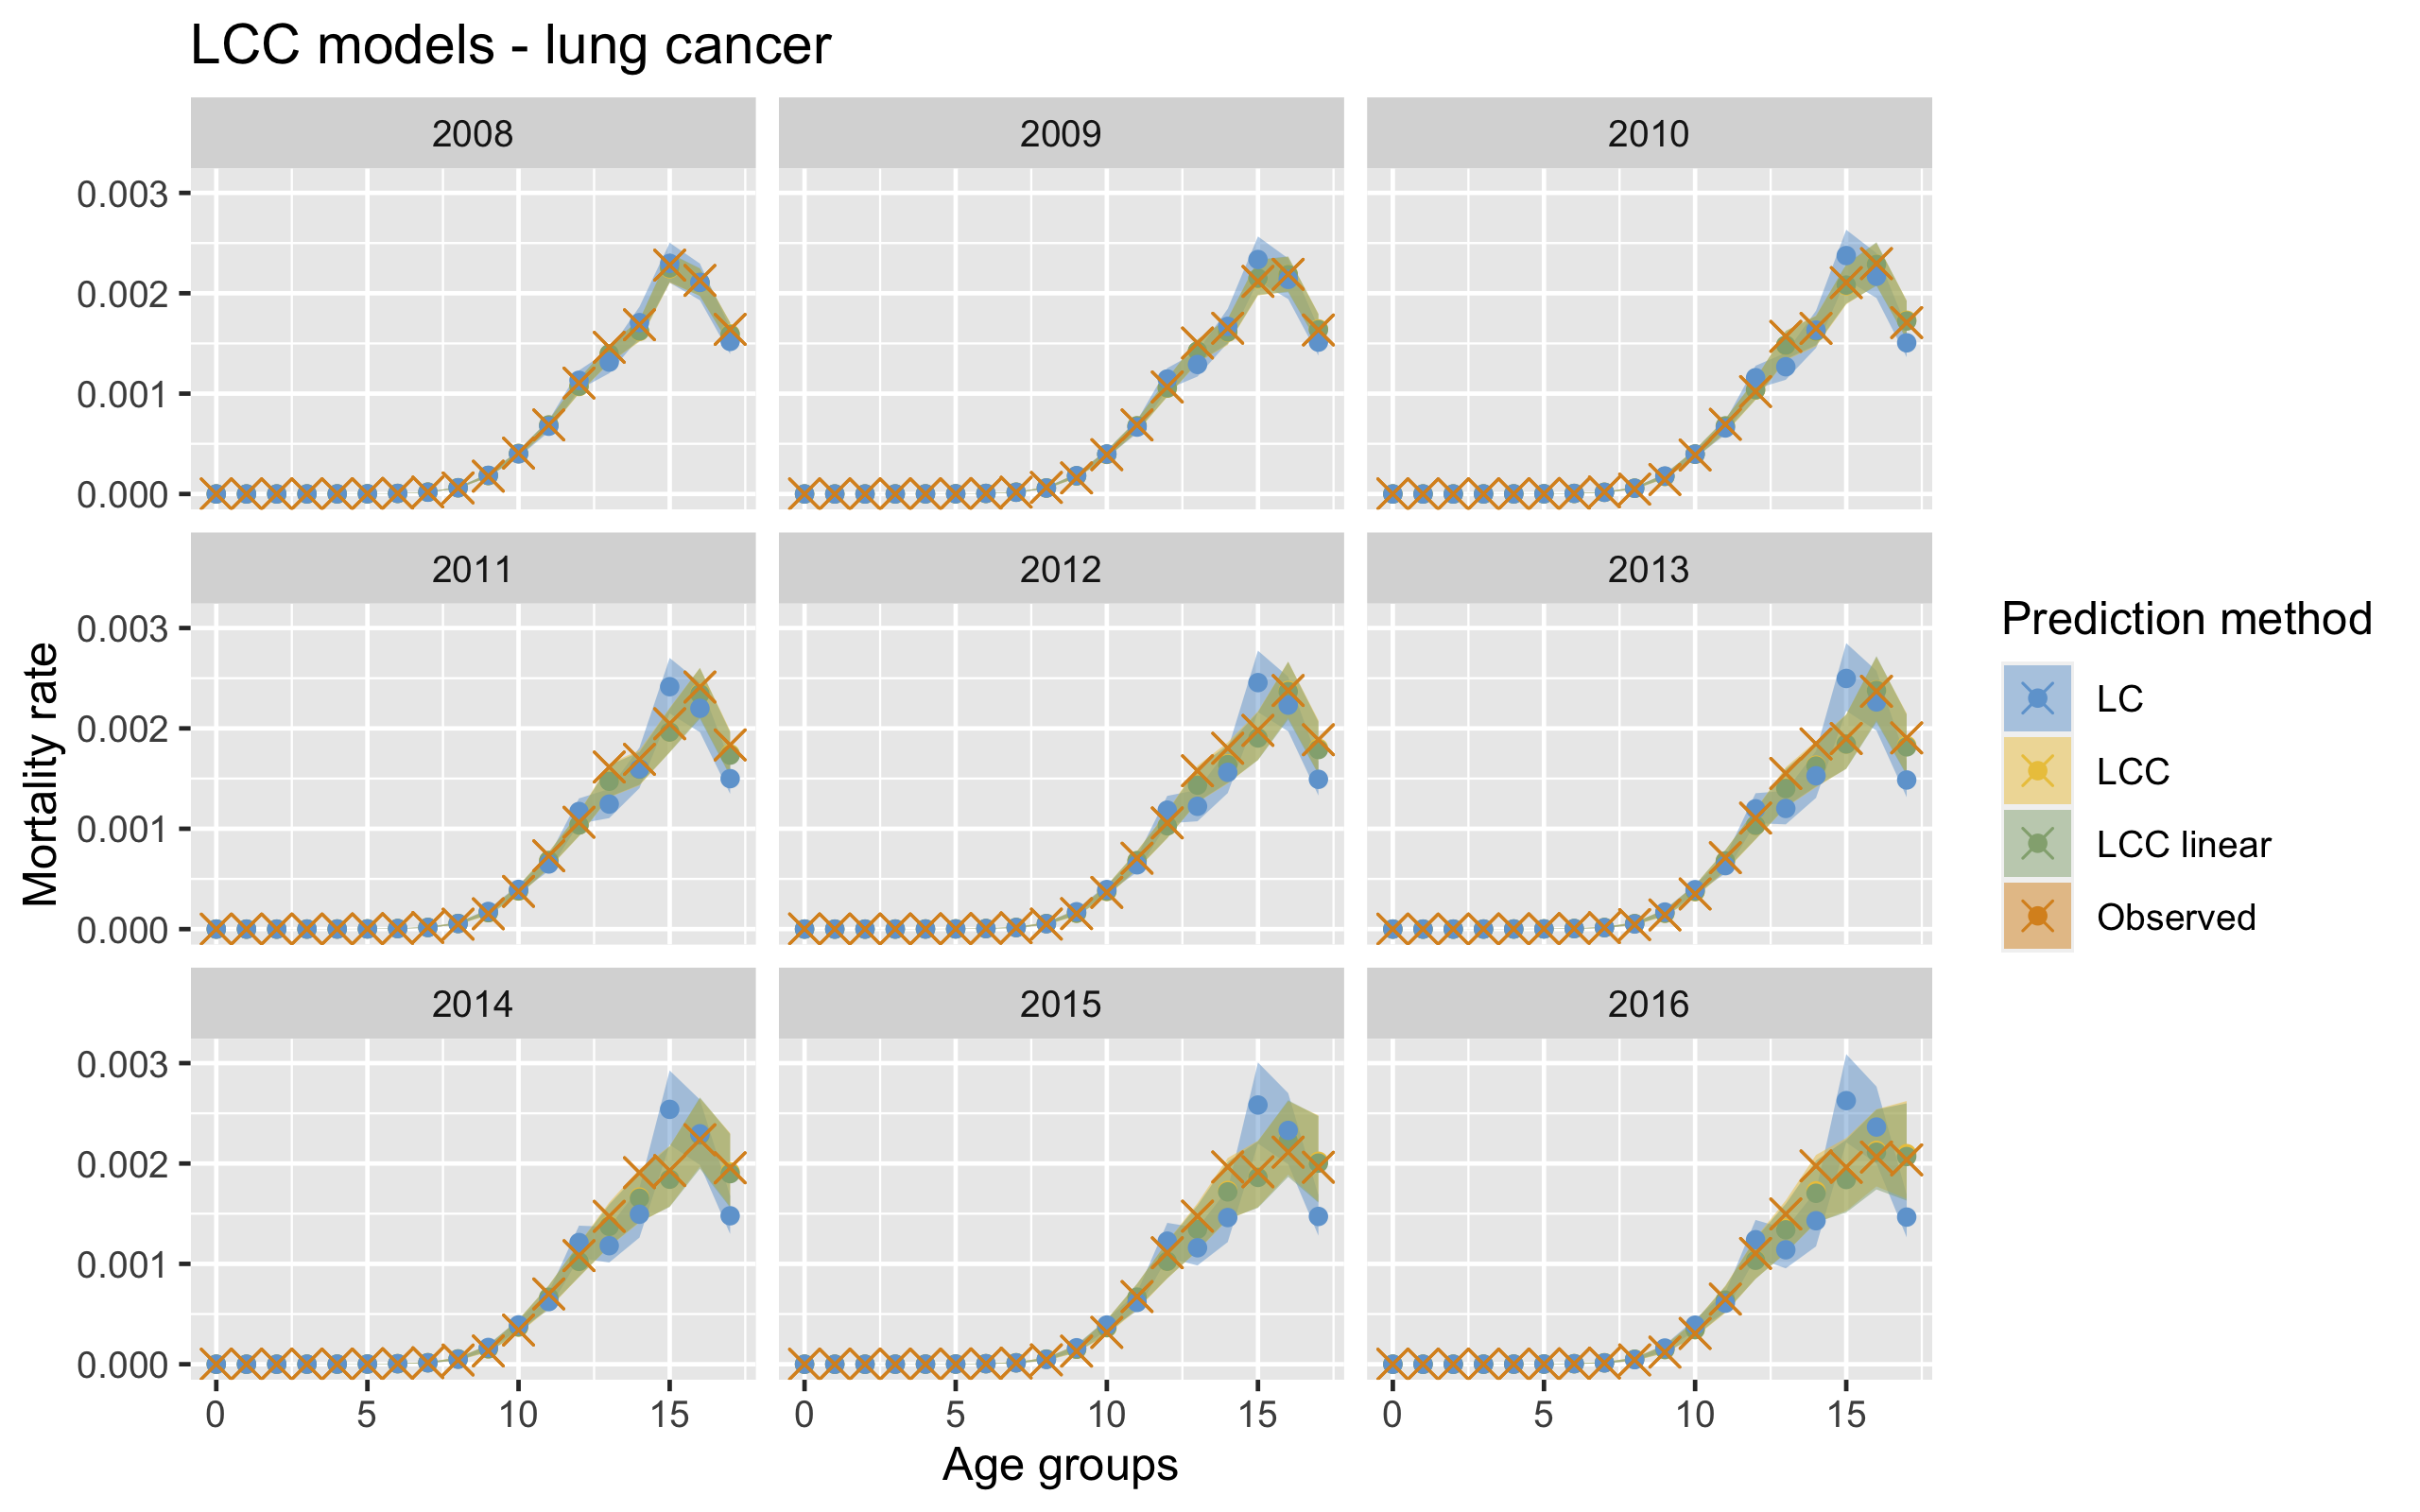
\includegraphics[width=\linewidth]{real-data/real-data-univariate/Figures/univariate-LCC-by-age-lung.png}
    \end{subfigure}
    \begin{subfigure}[b]{.45\linewidth}
        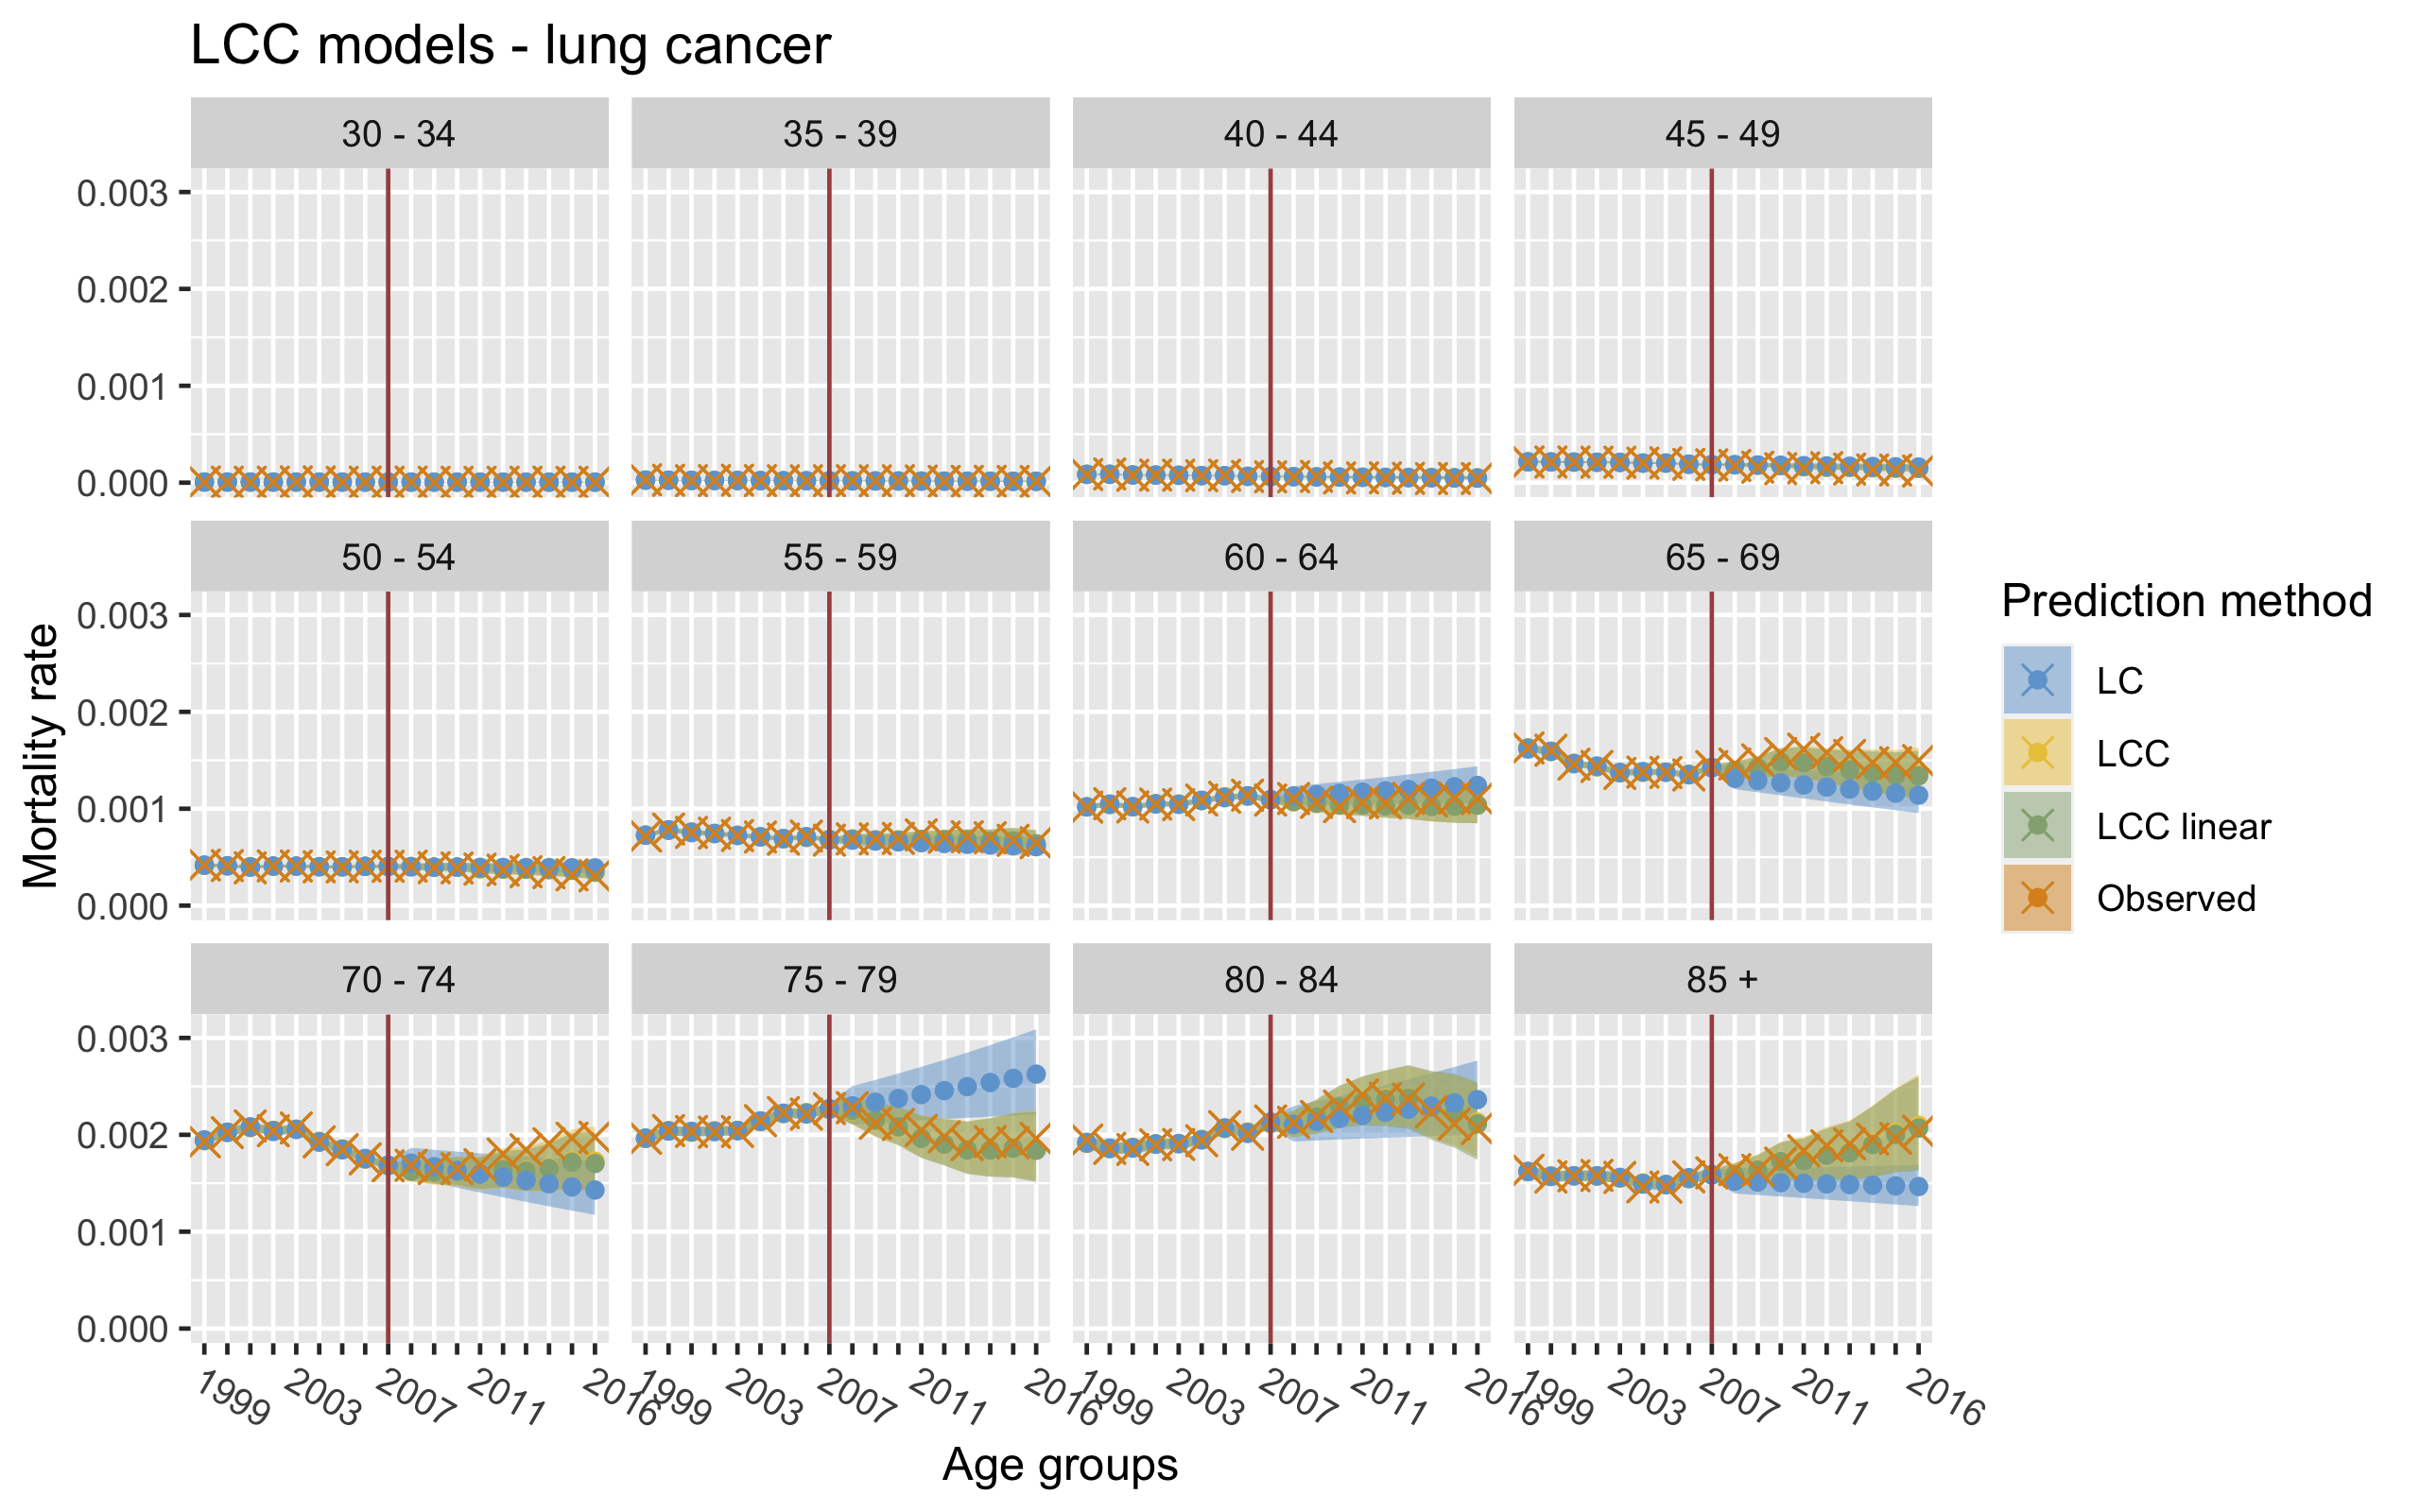
\includegraphics[width=\linewidth]{real-data/real-data-univariate/Figures/univariate-LCC-by-period-lung.png}
    \end{subfigure}
    \caption{Prediction results from inference with the Lee-Carter types of models on the lung cancer data set.}
    \label{fig:uv-LCC-lung}
\end{figure}

\begin{figure}[h!]
    \centering
    \begin{subfigure}[b]{.45\linewidth}
        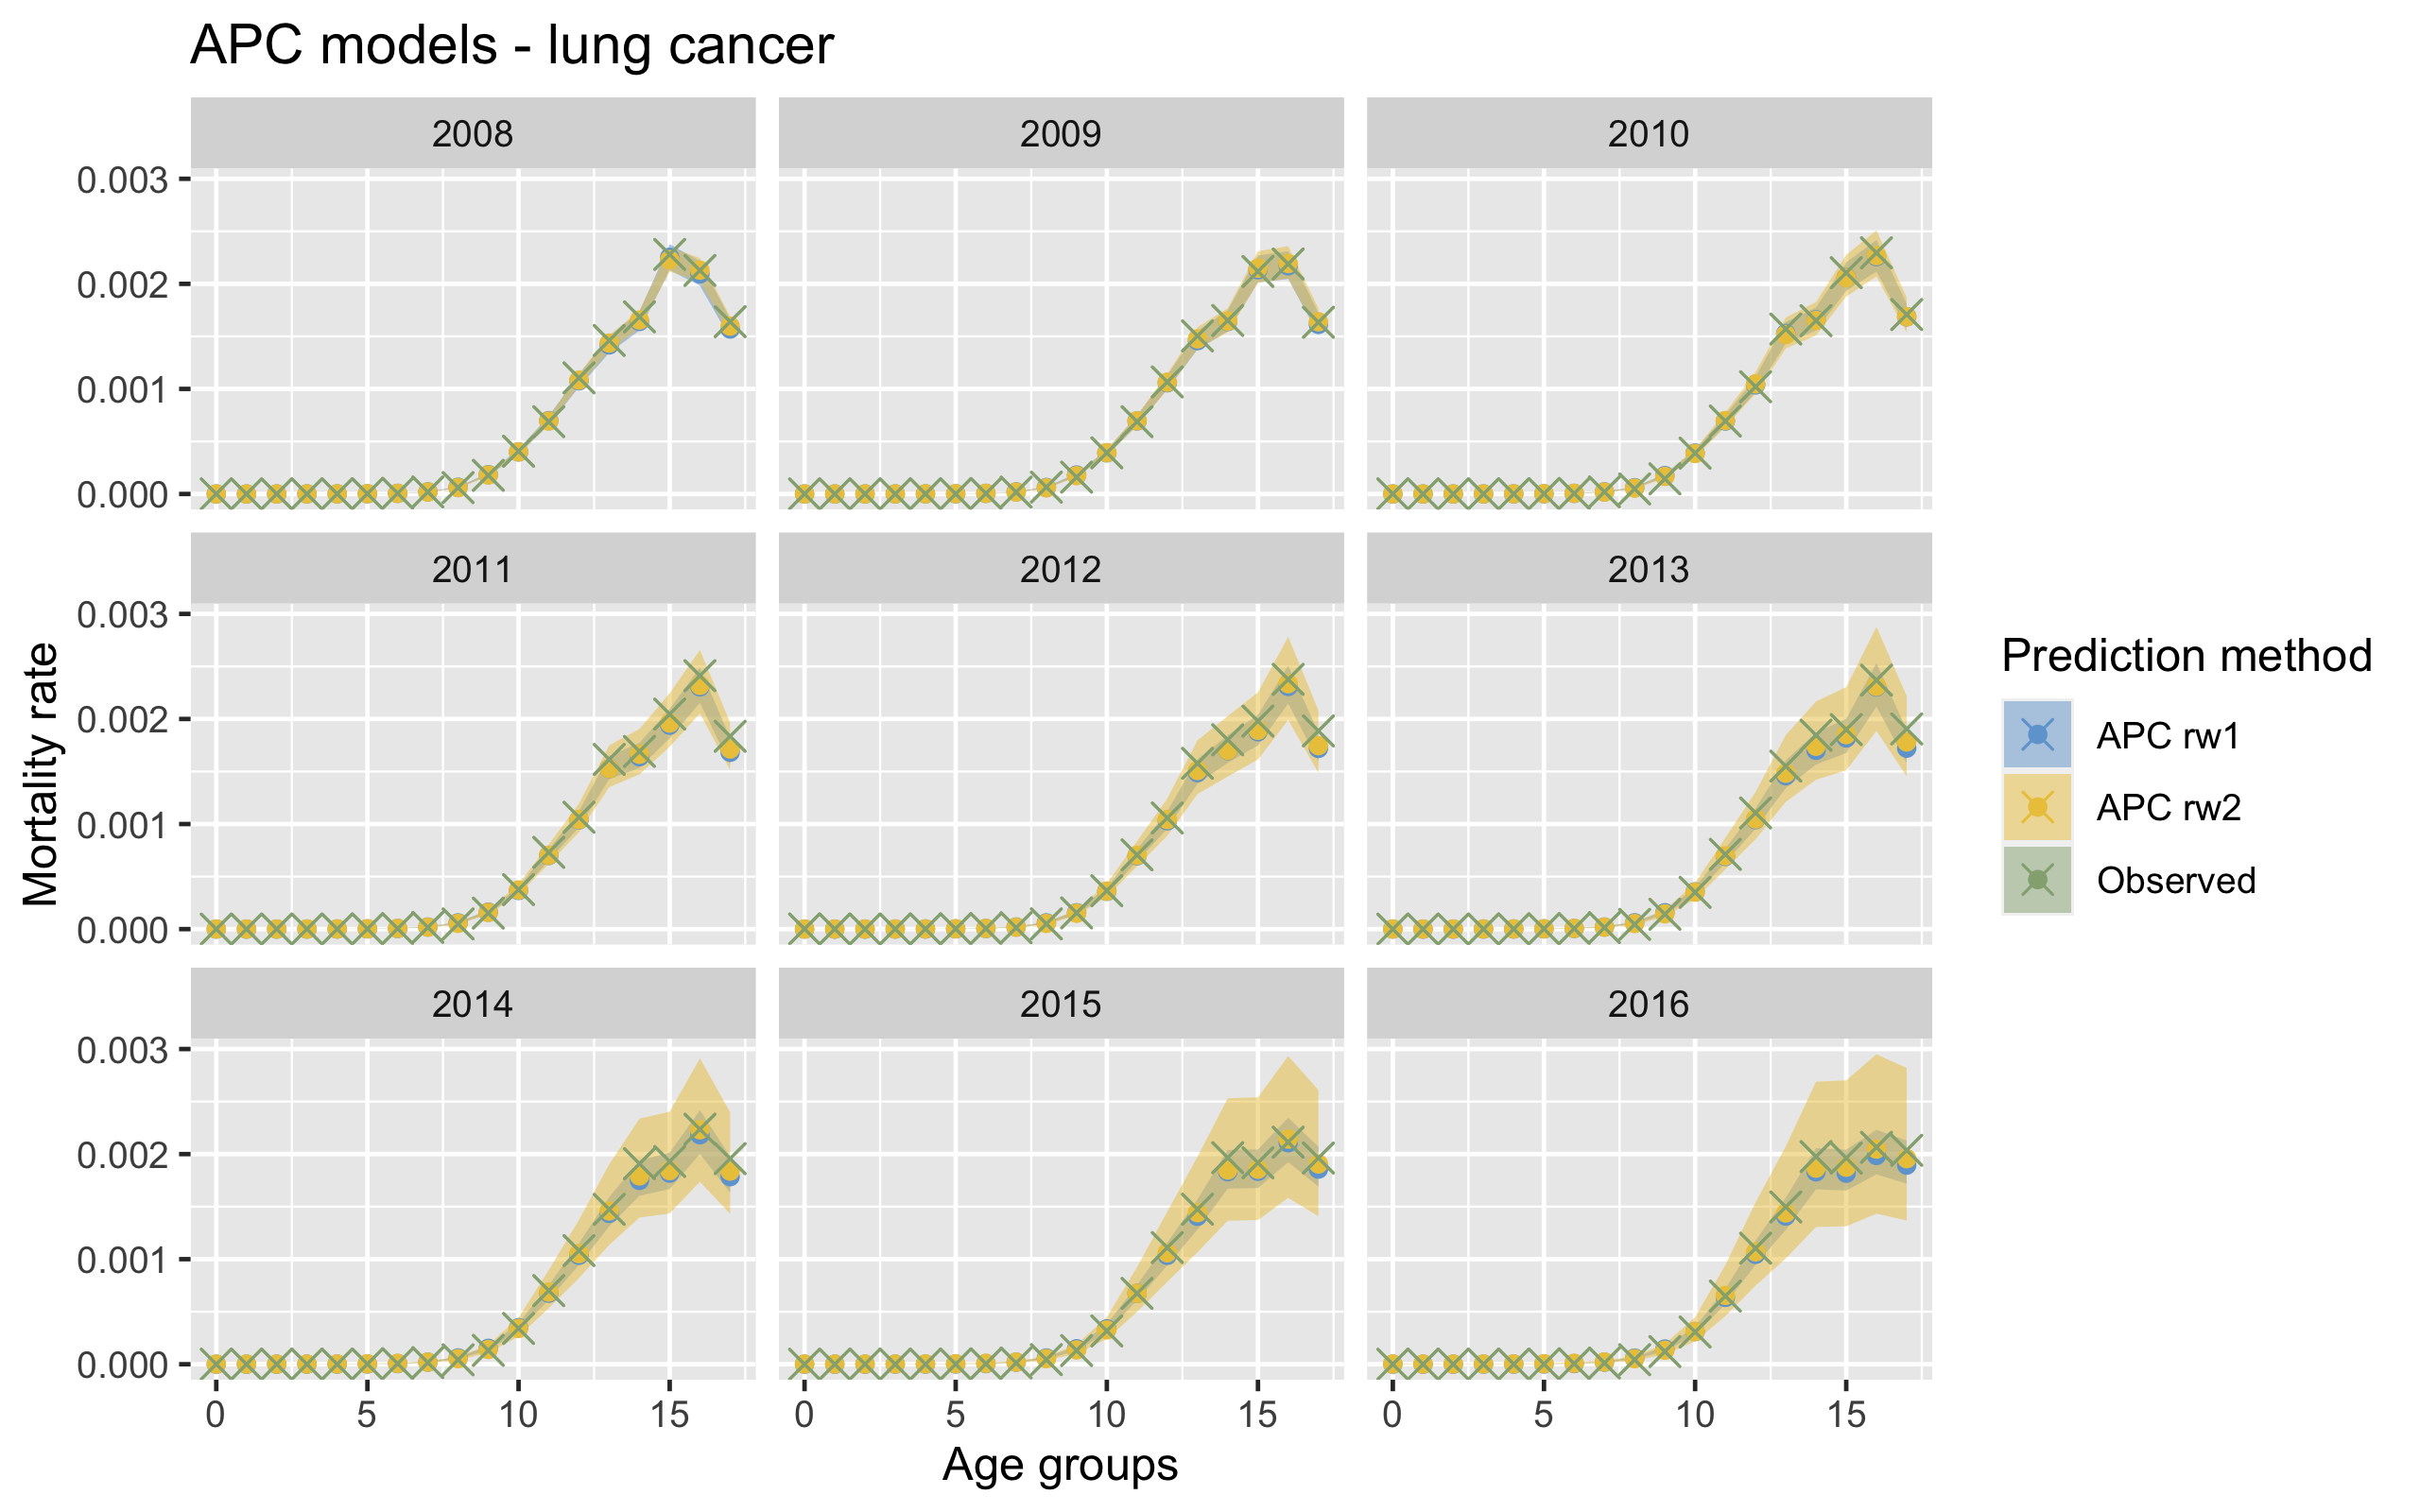
\includegraphics[width=\linewidth]{real-data/real-data-univariate/Figures/univariate-APC-by-age-lung.png}
    \end{subfigure}
    \begin{subfigure}[b]{.45\linewidth}
        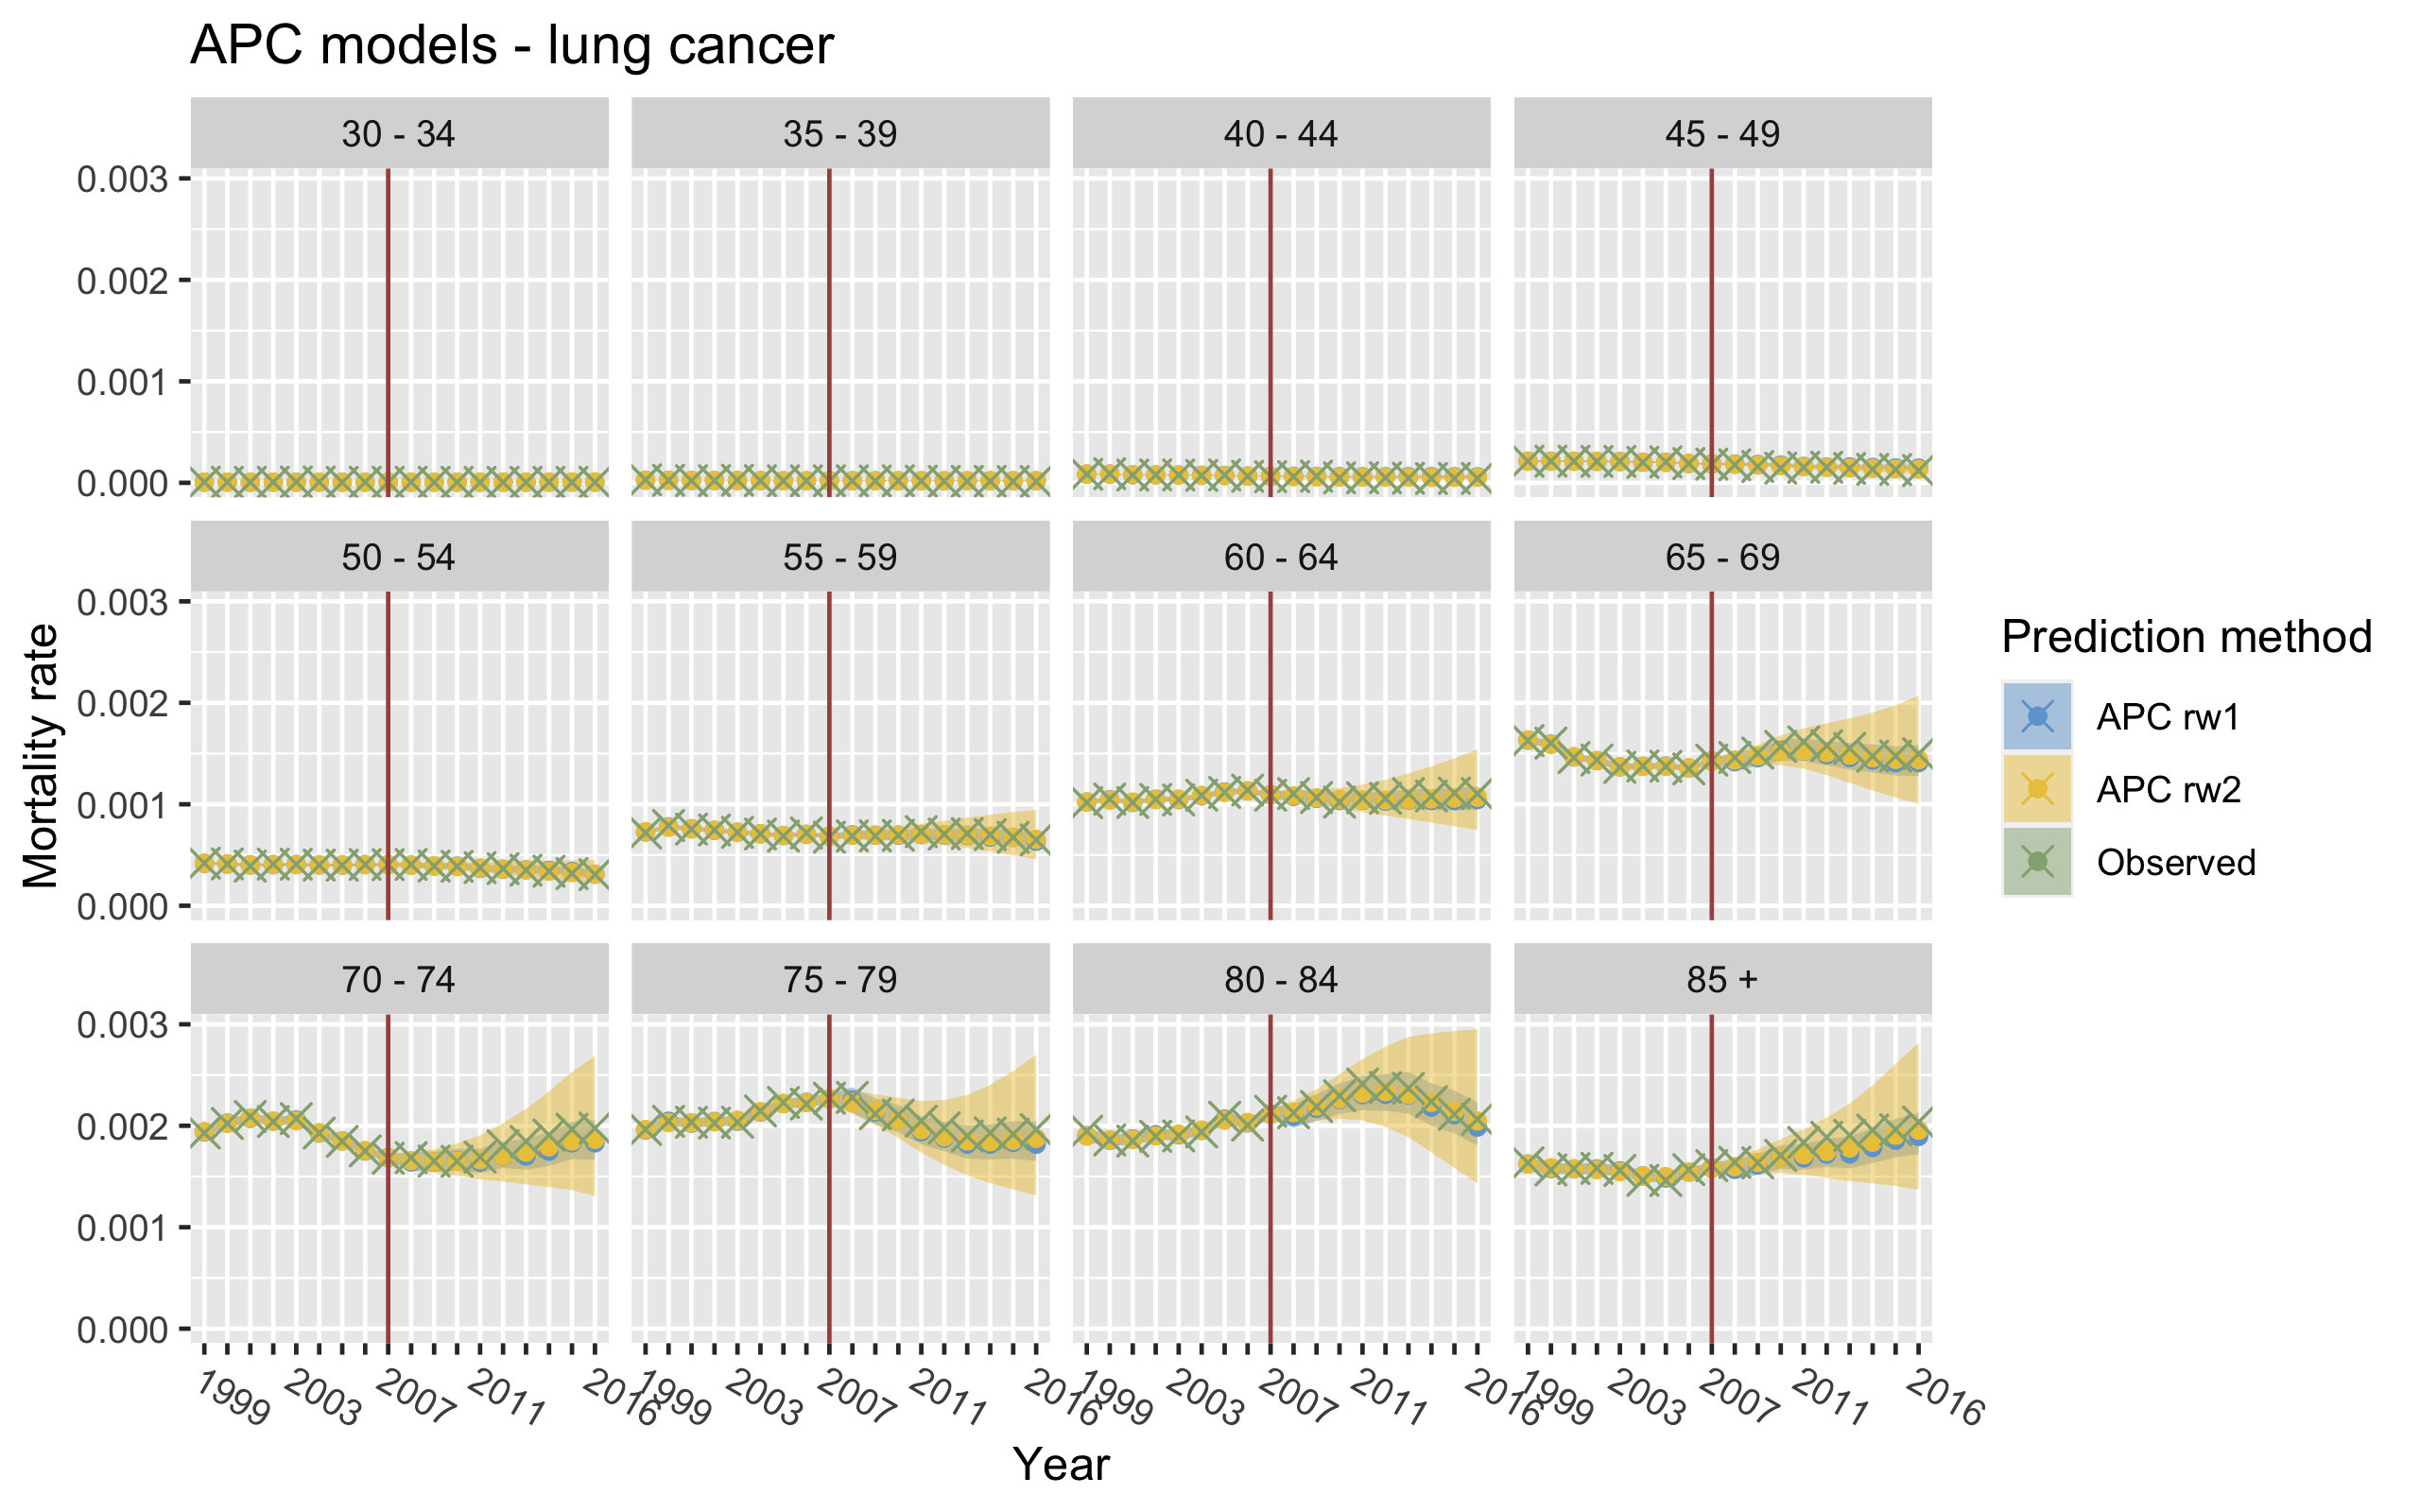
\includegraphics[width=\linewidth]{real-data/real-data-univariate/Figures/univariate-APC-by-period-lung.png}
    \end{subfigure}
    \caption{ Prediction results from inference with the APC types of models on the lung cancer data set.}
    \label{fig:uv-APC-lung}
\end{figure}

\begin{table}[h!]
    \begin{center}
        \begin{tabular}{l |c c c }
            Model & MSE &   MDSS & Contained 95\%-interval\\
            \hline
            APC1    & 3.896e-9 & -19.27    & 0.7778 \\
            APC2    & 2.174e-9 & -19.88    & 0.8889 \\
            LC      & 5.144e-8 & -16.02    & 0.6204 \\
            LCC     & 4.746e-9 & -20.12    & 0.9907 \\
            LCC-linear      & 5.238e-9 & -20.01    & 0.9722 \\
        \end{tabular}
        \caption{Lung cancer data, cutoff at x <= 5}\label{tbl:uv-lung-5}
    \end{center}
\end{table}

\newpar Figures \ref{fig:uv-LCC-lung} and \ref{fig:uv-APC-lung} display the prediction results for lung cancer mortality, using the Lee-Carter and the APC methods, respectively. We present the predictions for each predicted year, with age groups along the x-axis (the left-most image in the figures) and for each age group, with all years along the x-axis (right-most image in the figures). For the images where results are displayed by age groups, we only show the results for ages above 30. This is simply because the real and predicted mortality rates are very close to zero for younger ages, so these results are not very interesting. The red line marks the division between fitted and predicted mortality rates. The score statistics for these results are displayed in Table \ref{tbl:uv-lung-5}. Figures \ref{fig:uv-LCC-stomach} and \ref{fig:uv-APC-stomach} and Table \ref{tbl:uv-stomach-5} show the same results for predictions of stomach cancer mortality. 
\newpar
First of all, we observe that Figures \ref{fig:uv-LCC-lung} and \ref{fig:uv-LCC-stomach} confirm the results from Section \ref{sec:SyntheticData} that it is possible to fit Lee-Carter models to mortality data using \inlabru, as all Lee-Carter models seem to fit the observed data well for the years that are not predicted. Furthermore, we observe that for both lung and stomach cancer, the LCC and LCC-linear models perform significantly better than the LC-model. This difference is especially apparent for the older age groups. The LCC- and the LCC-linear models seem, from the plotted results, to give very similar, and quite good, predictions. These observations are confirmed by the score statistics in Tables \ref{tbl:uv-lung-5} and \ref{tbl:uv-stomach-5}. The MDSS for the LC-model is clearly higher than the MDSS for the LCC and the LCC-linear models, which is a clear indication that the LC-model performs worse than the others. \textcolor{myDarkGreen}{The LCC and the LCC-linear models have very similar score statistics. The MDSS for the LCC model is slightly lower than the MDSS for the LCC-linear model, both for lung and stomach cancer, indicating that the former gives better predictions. Since this was our original proposed model, and we do not seem to gain performance in prediction by omitting the non-linear period term $\kappa_t$, we keep this model in our following investigation. Still, we underline that it seems like most of the period-related variability in the mortality rates can be explained by a linear trend. }

\begin{figure}[h!]
    \centering
    \begin{subfigure}[b]{.45\linewidth}
        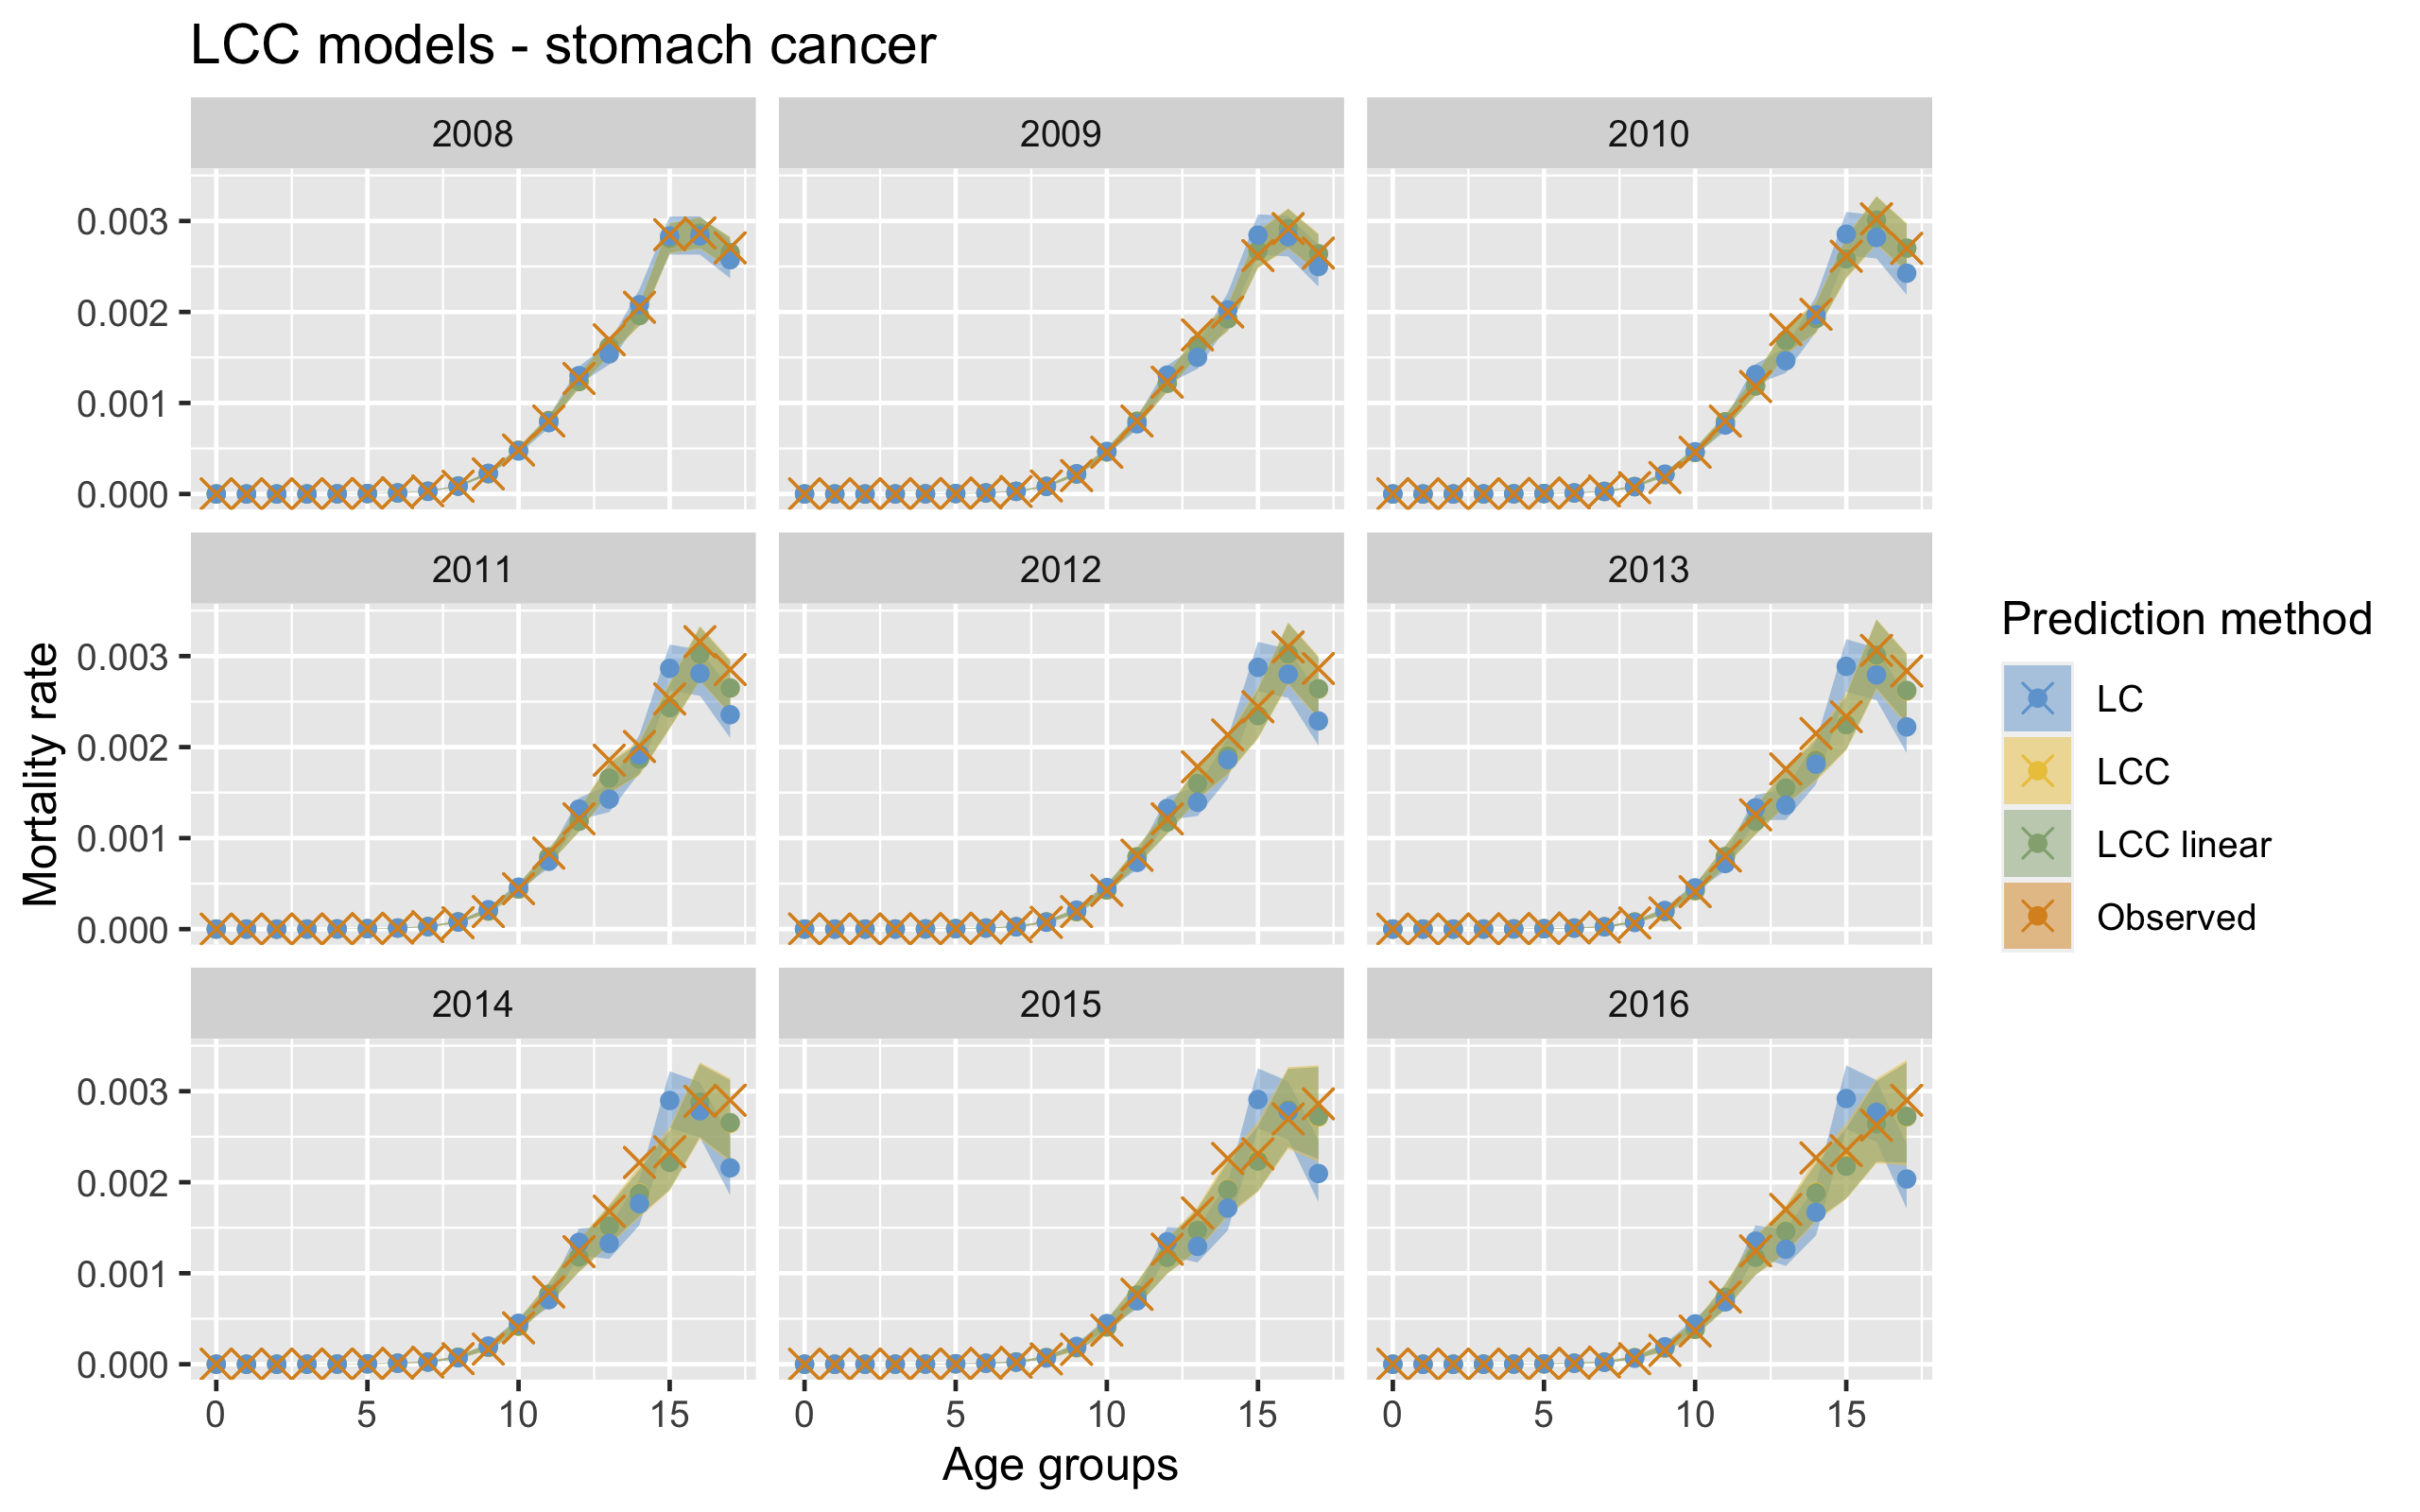
\includegraphics[width=\linewidth]{real-data/real-data-univariate/Figures/univariate-LCC-by-age-stomach.png}
    \end{subfigure}
    \begin{subfigure}[b]{.45\linewidth}
        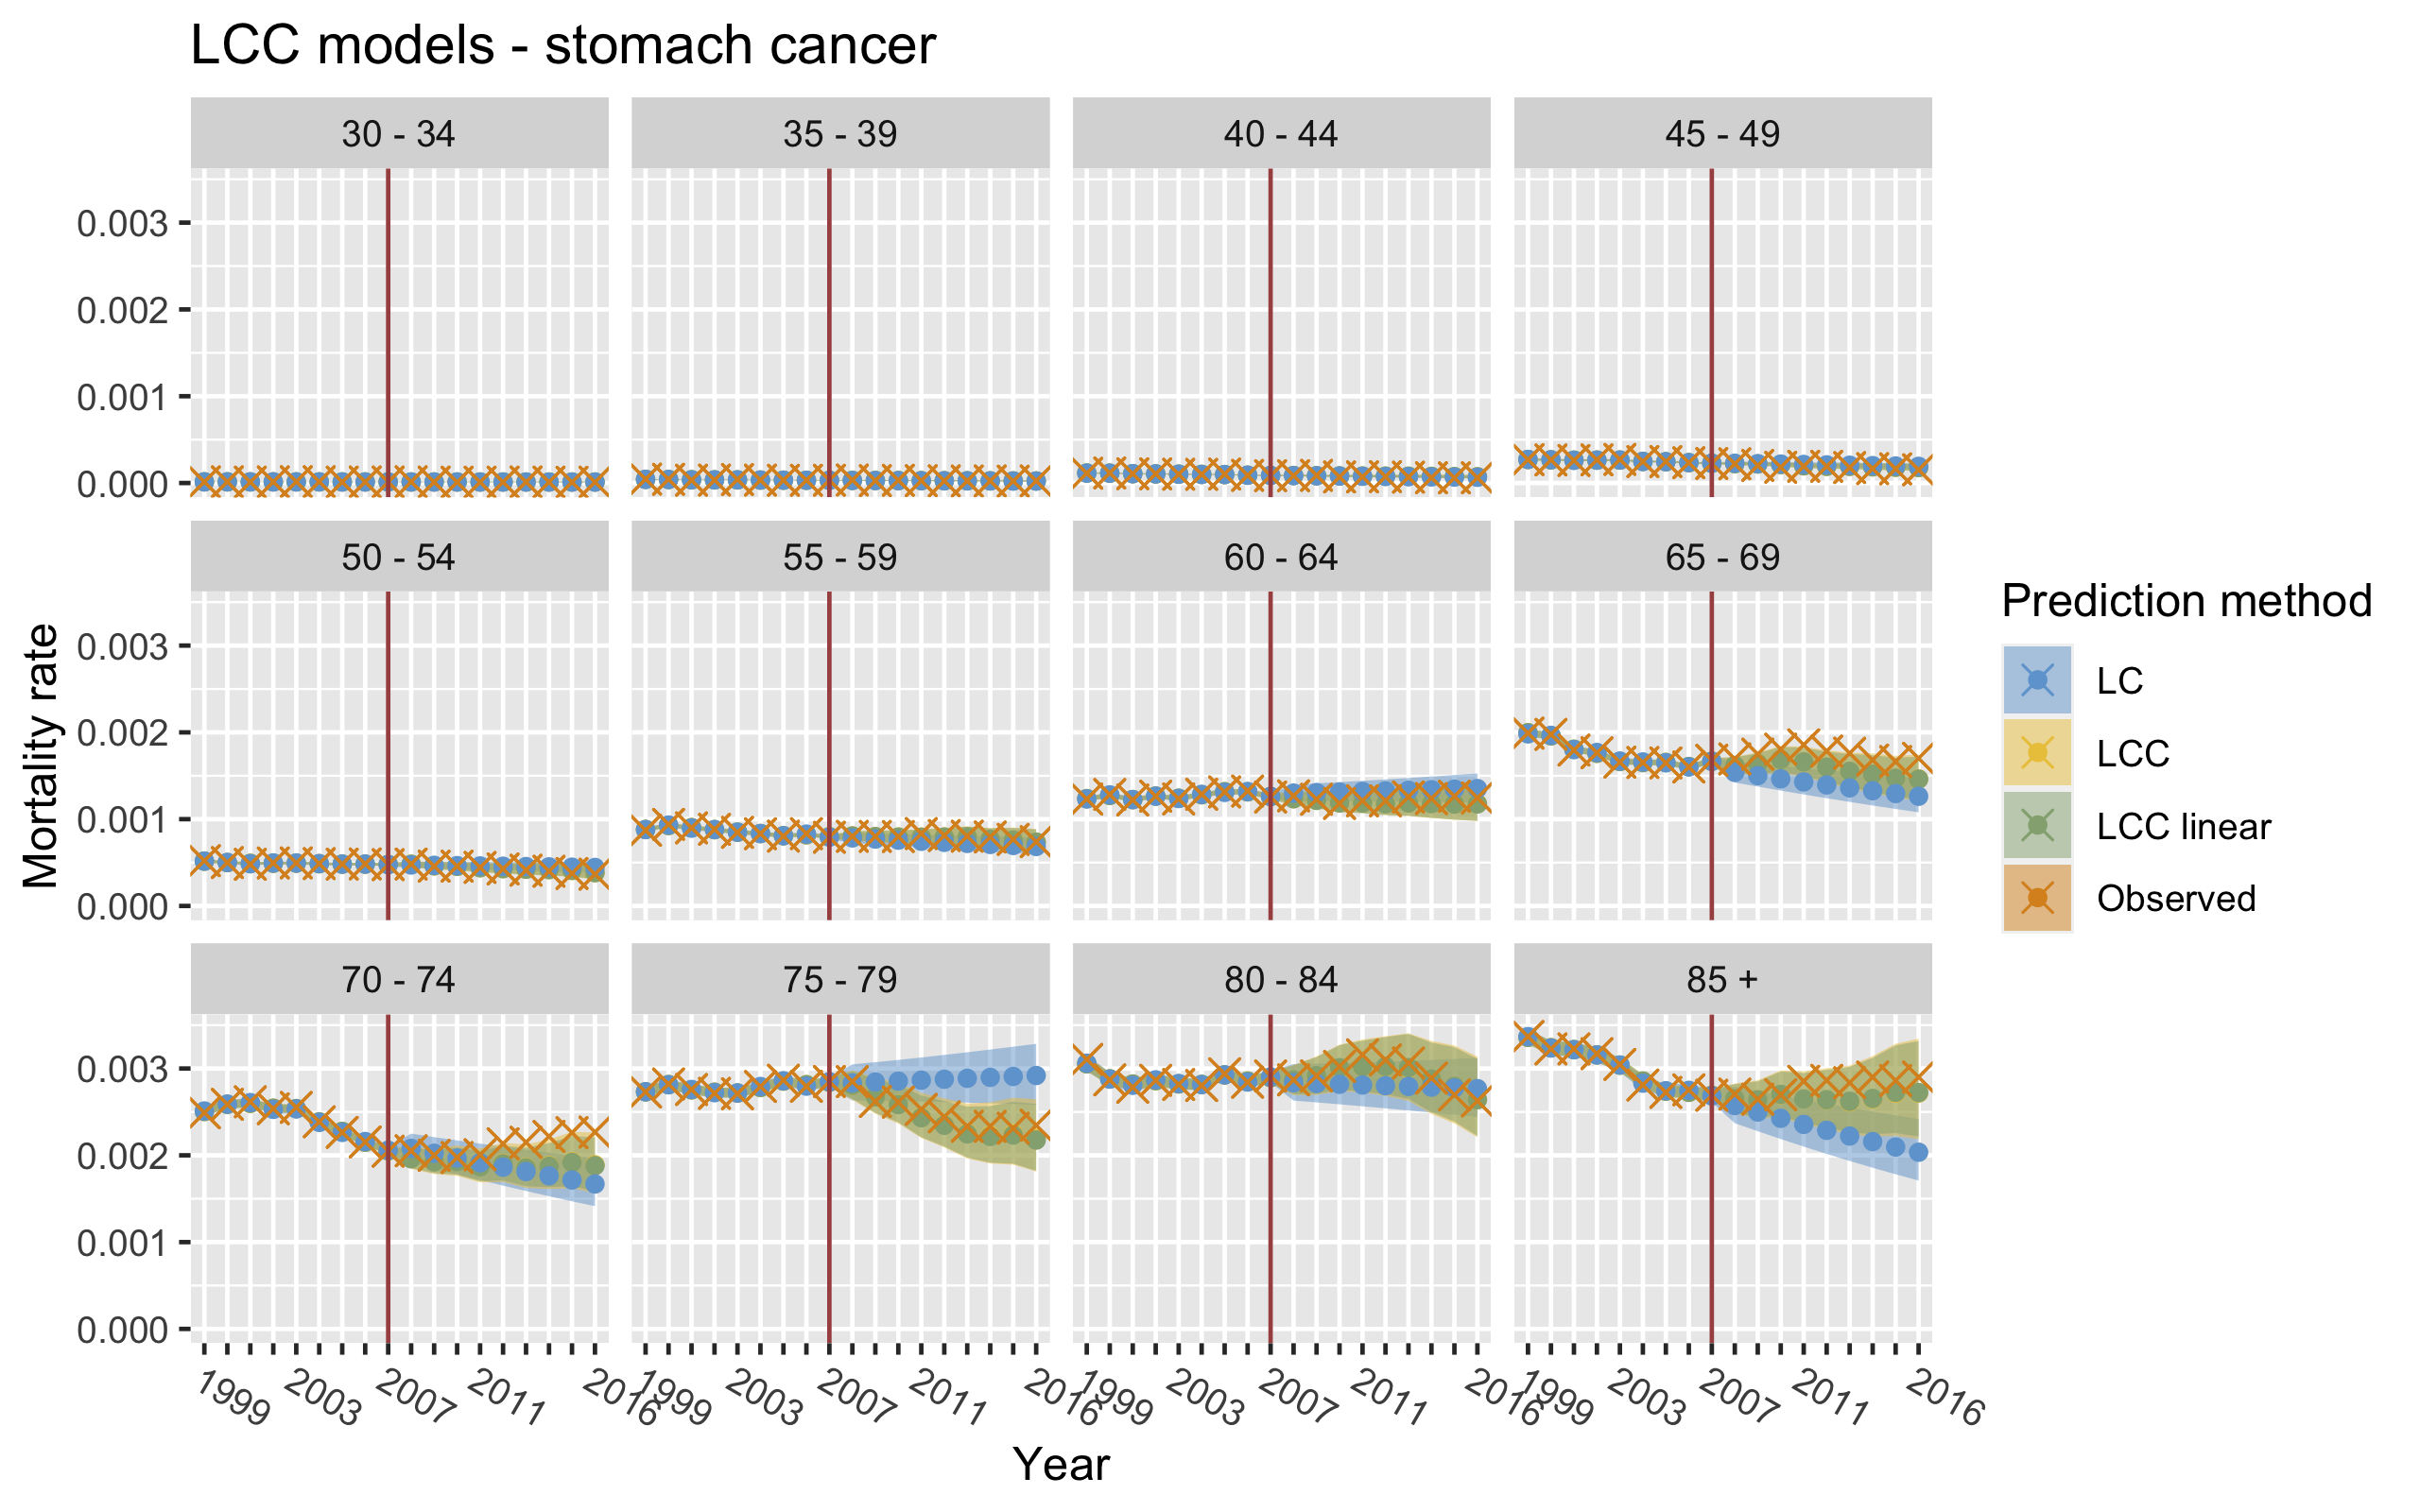
\includegraphics[width=\linewidth]{real-data/real-data-univariate/Figures/univariate-LCC-by-period-stomach.png}
    \end{subfigure}
    \caption{Prediction results from inference with the Lee-Carter types of models on the stomach cancer data set.}
    \label{fig:uv-LCC-stomach}
\end{figure}

\begin{figure}[h!]
    \centering
    \begin{subfigure}[b]{.45\linewidth}
        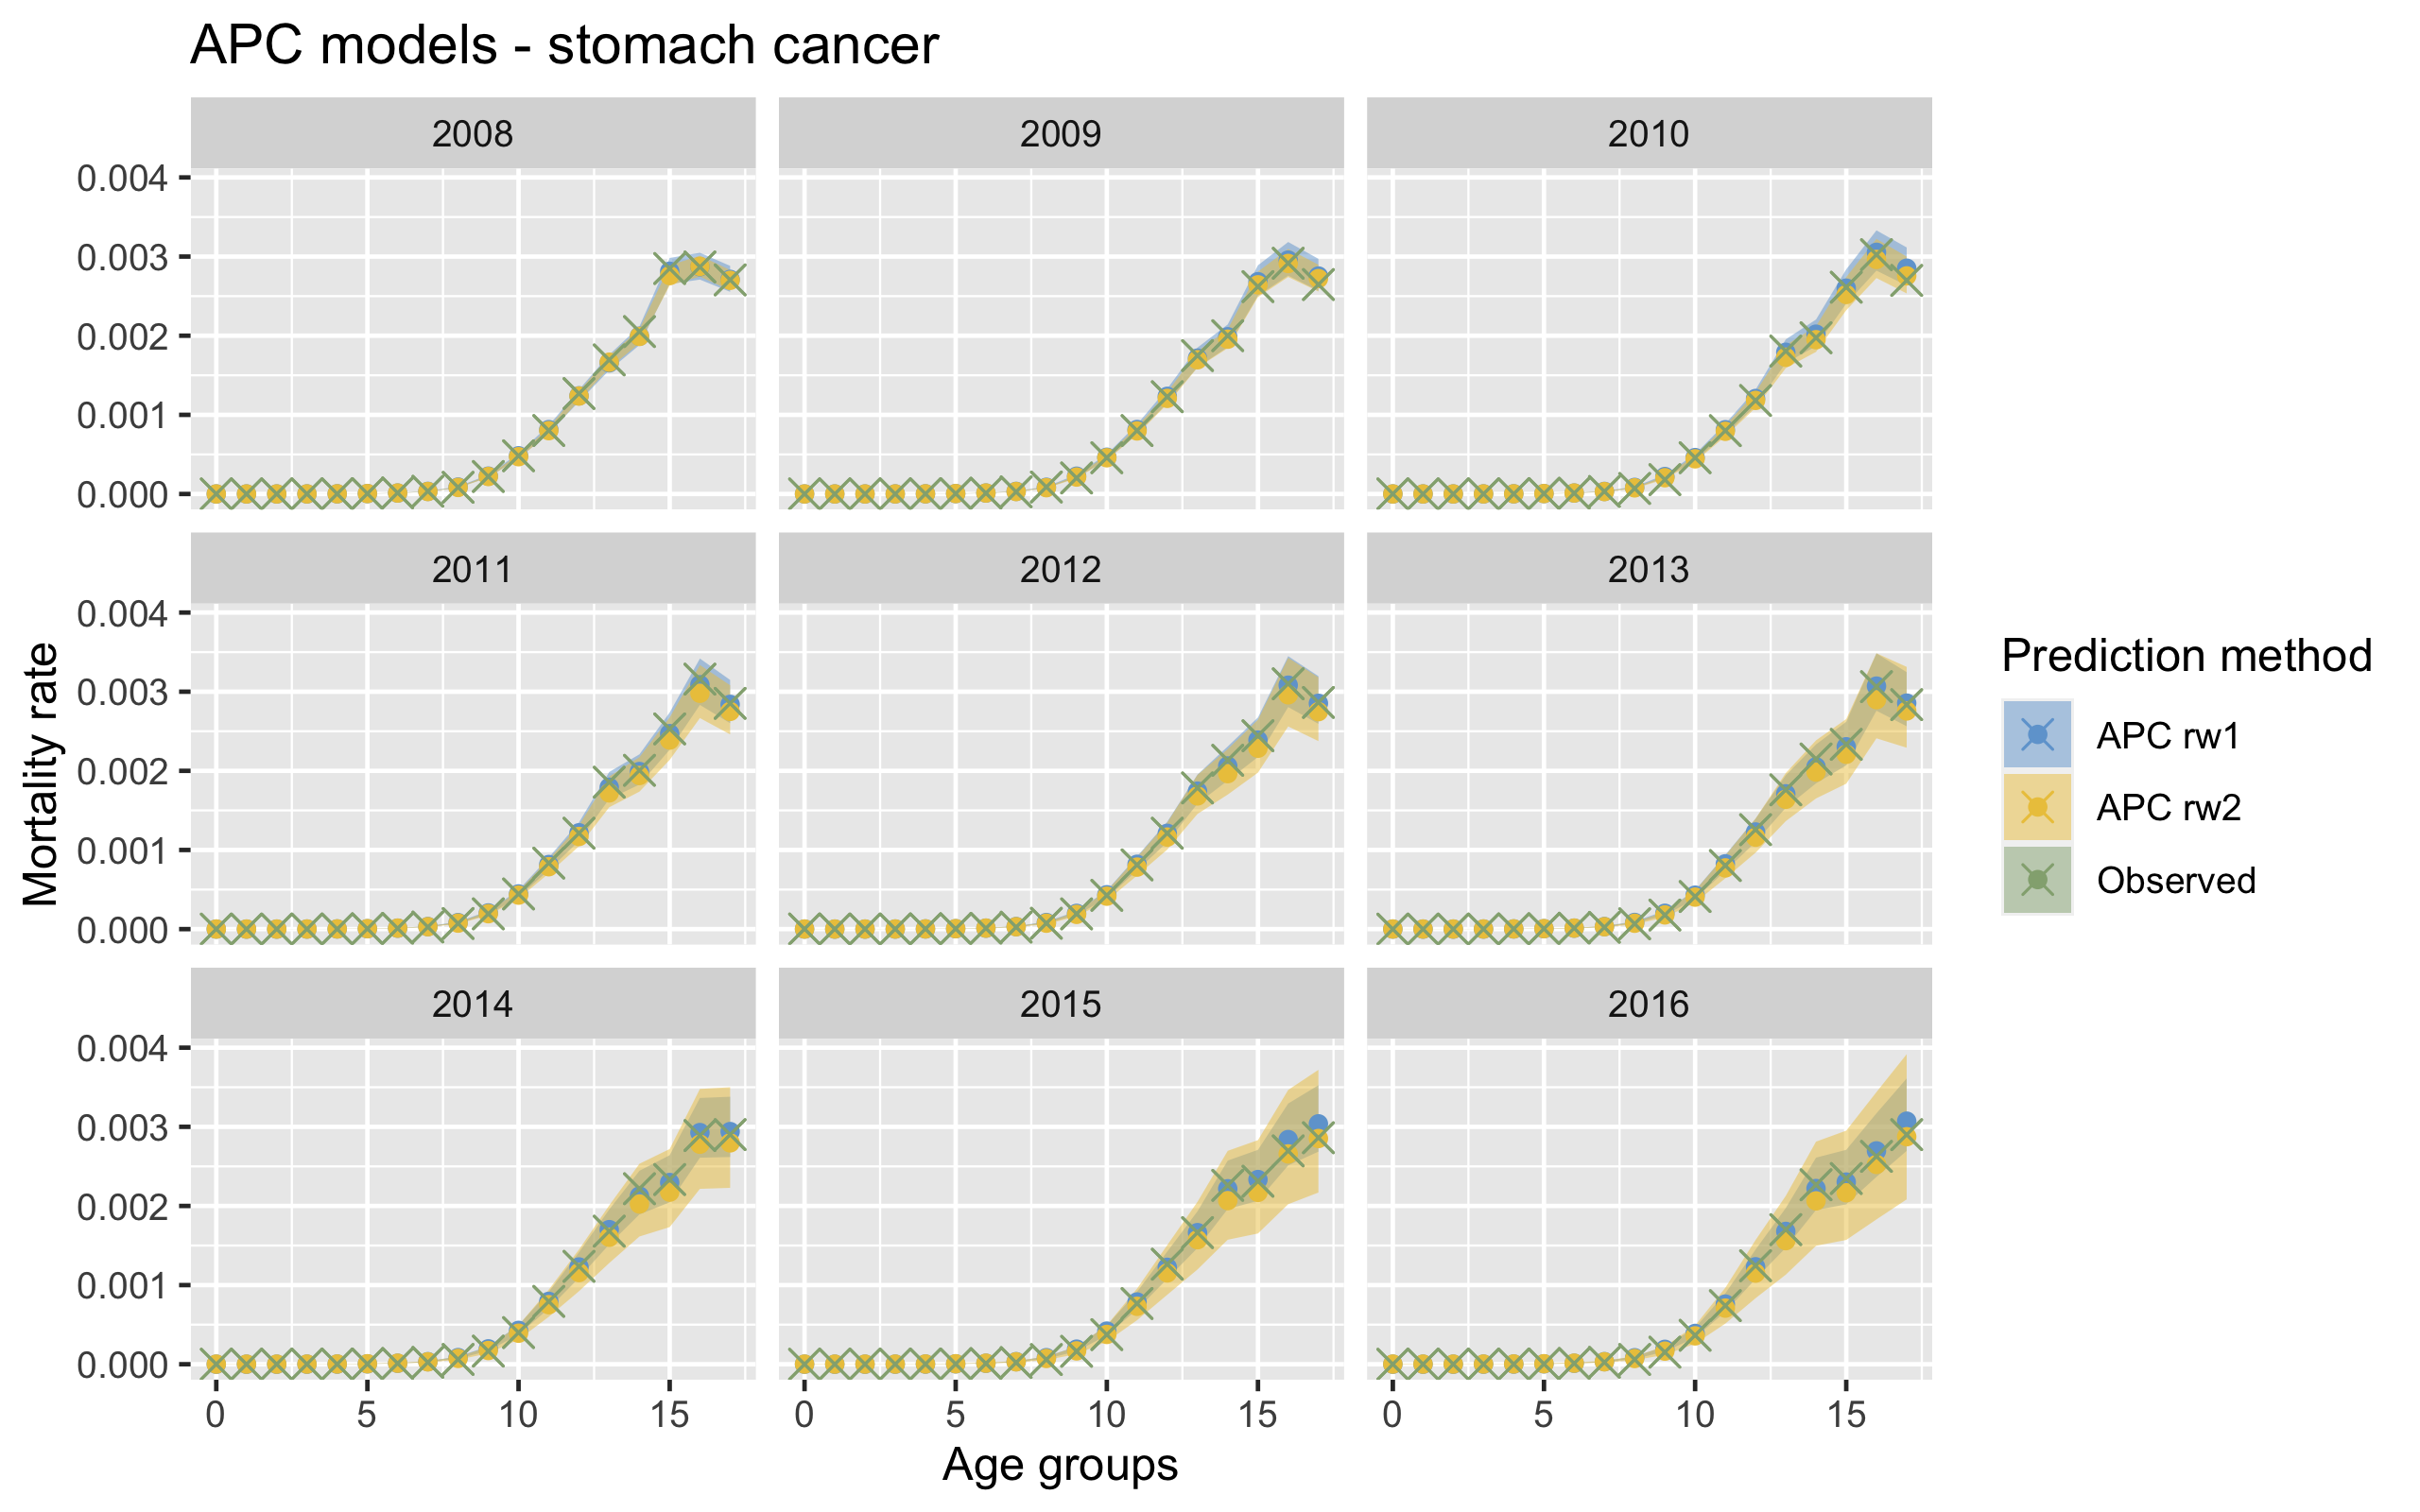
\includegraphics[width=\linewidth]{real-data/real-data-univariate/Figures/univariate-APC-by-age-stomach.png}
    \end{subfigure}
    \begin{subfigure}[b]{.45\linewidth}
        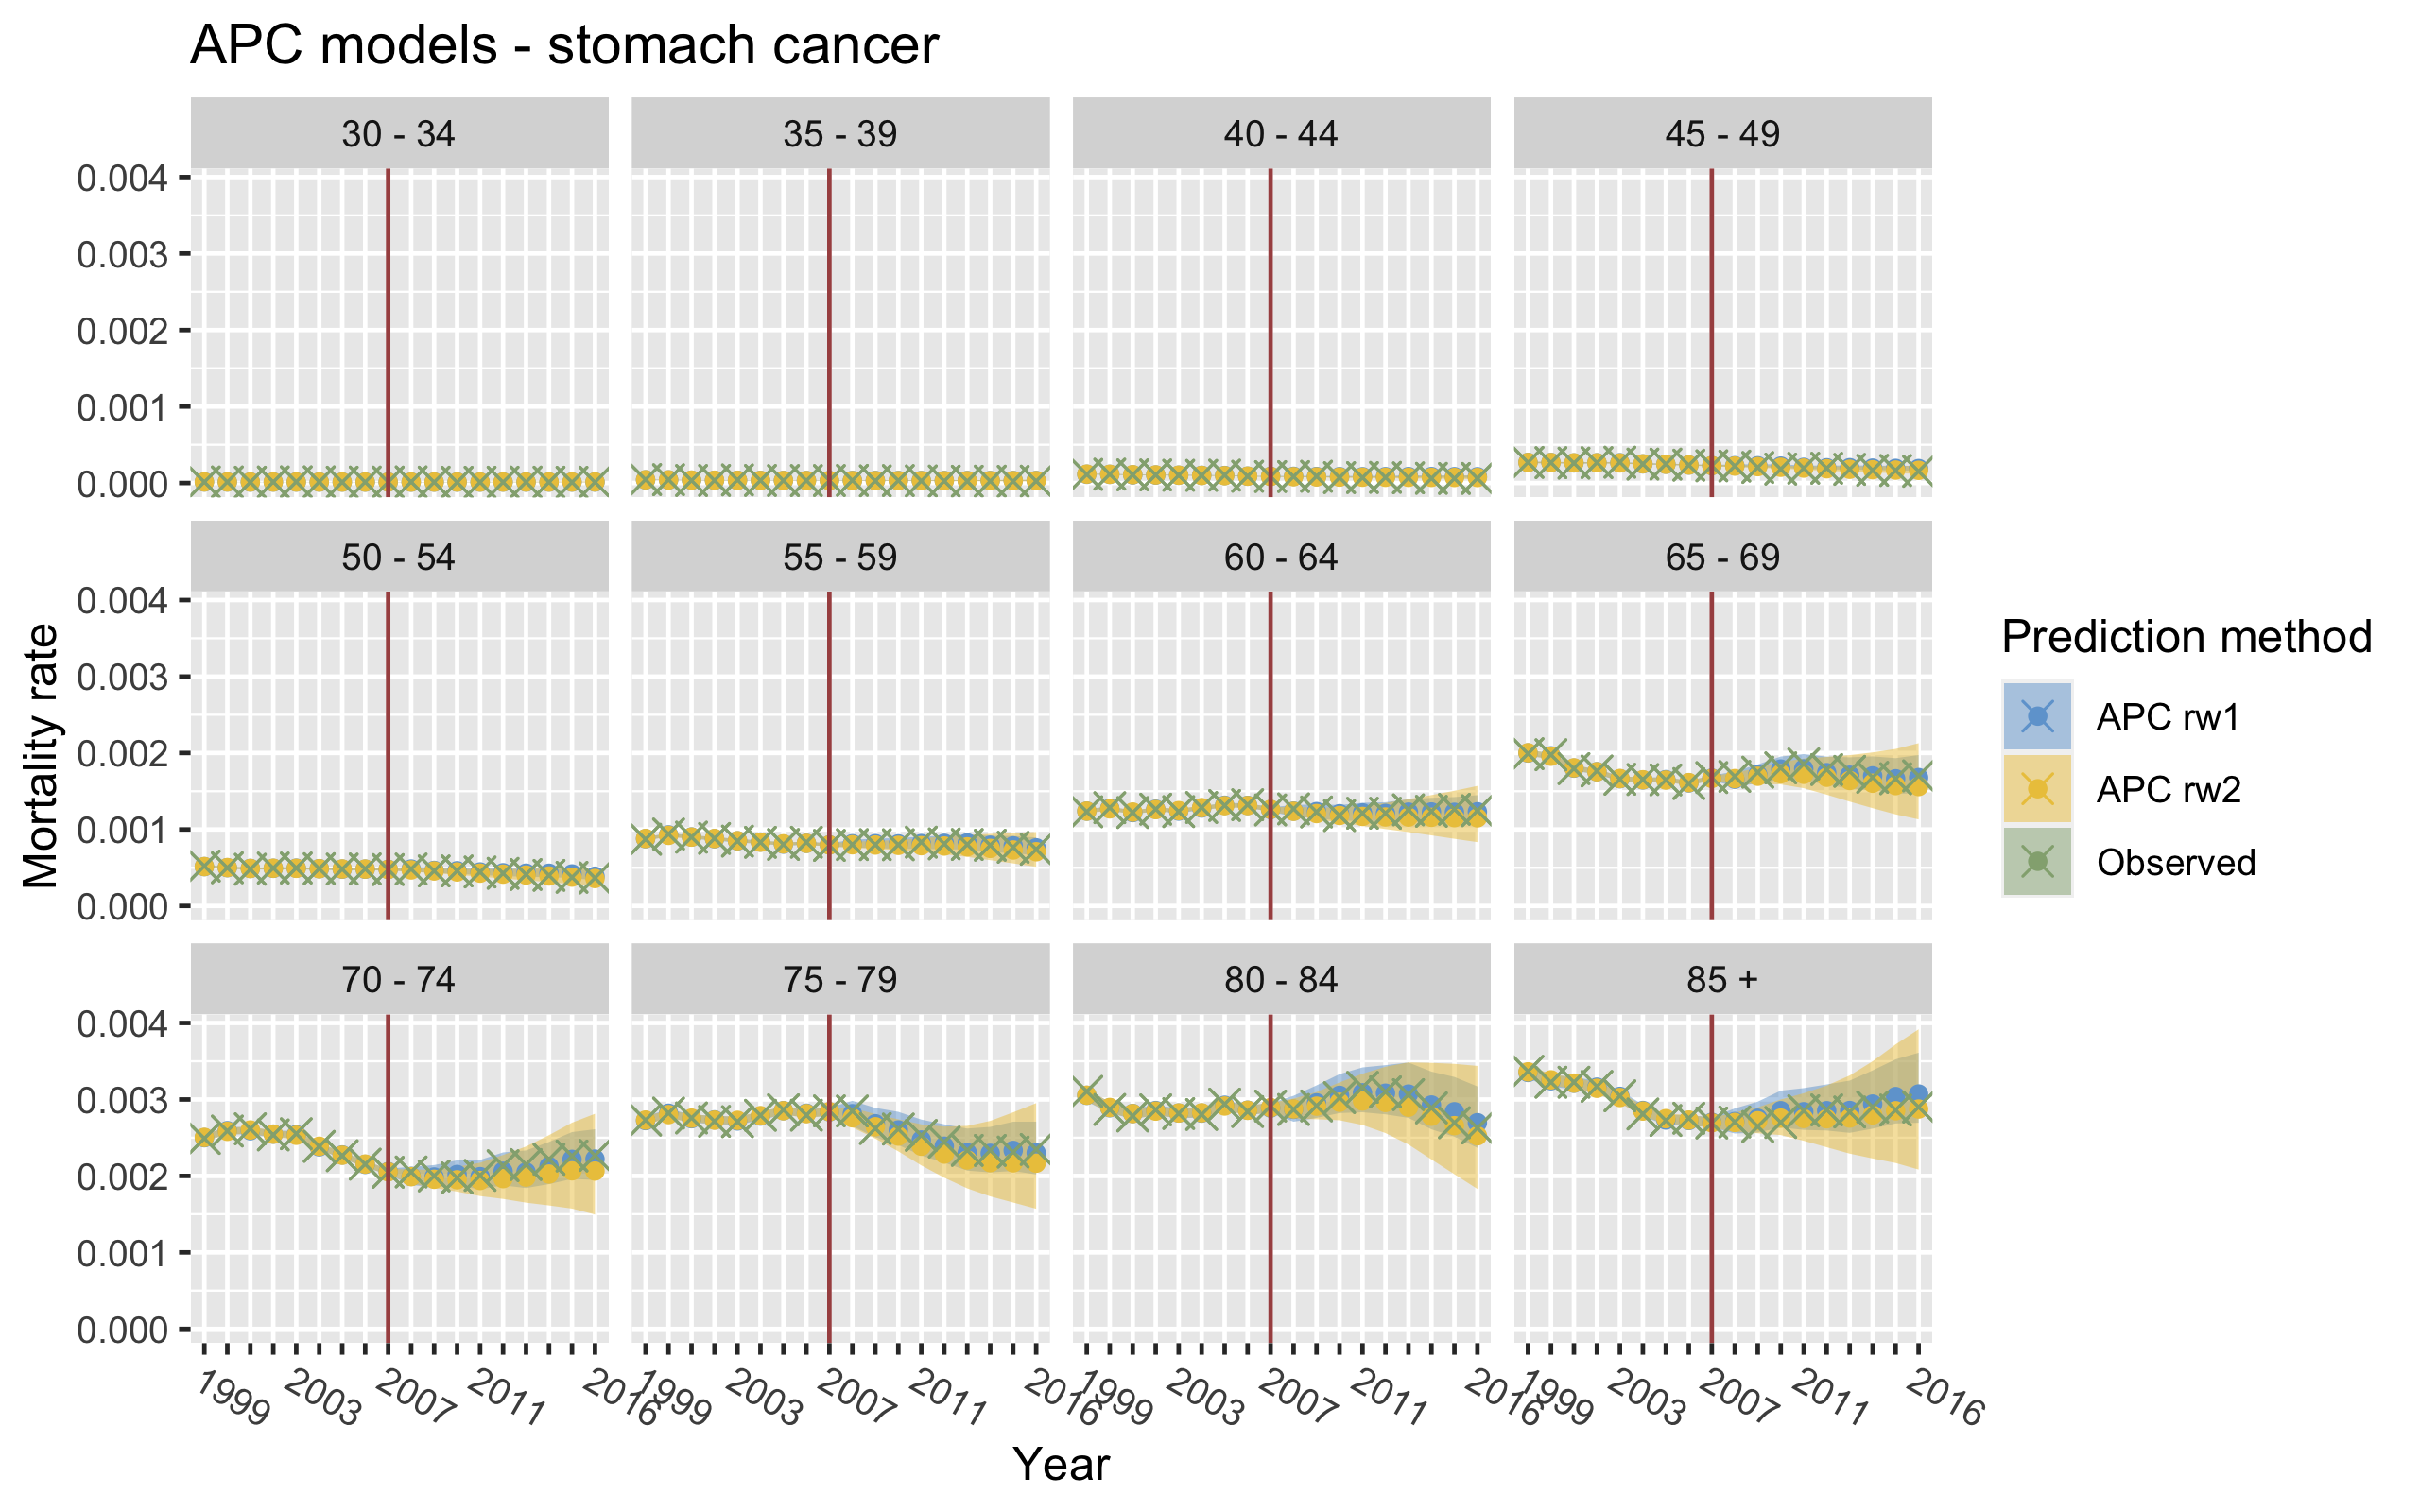
\includegraphics[width=\linewidth]{real-data/real-data-univariate/Figures/univariate-APC-by-period-stomach.png}
    \end{subfigure}
    \caption{Prediction results from inference with the APC types of models on the stomach cancer data set.}
    \label{fig:uv-APC-stomach}
\end{figure}

\begin{table}[h!]
    \begin{center}
        \begin{tabular}{l |c c c }
            Model & MSE &   MDSS & Contained 95\%-interval\\
            \hline
            APC1     & 1.969e-9 & -19.12    & 0.7963 \\
            APC2     & 5.840e-9 & -19.52    & 0.9167 \\
            LC      & 6.851e-8 & -15.50    & 0.5926 \\
            LCC     & 1.112e-8 & -19.46    & 0.9352 \\
            LCC-linear      & 1.141e-8 & -19.39    & 0.8889
        \end{tabular}
        \caption{Stomach cancer data, cutoff at x <= 5}\label{tbl:uv-stomach-5}
    \end{center}
\end{table}

\newpar For the two APC models, APC1 and APC2, it is less clear which model perform the best. Figures \ref{fig:uv-APC-lung} and \ref{fig:uv-APC-stomach} display the results from using the APC models to predict lung and stomach cancer mortality. Firstly, we note that both the APC1 and APC2-models seem to predict the mortality rates well, both for lung and stomach cancer. We observe that for both cancer types, the APC2-model produces predictions with wider prediction intervals than the APC1-model does. We also observe that the prediction intervals from the APC2-model is widening with more recent years (the predictions get less sharp further into the future). This tendency is not as clear for the APC1-model. For lung cancer mortality, we observe from Figure \ref{fig:uv-APC-lung} that the APC2 predictions might be slightly more accurate than the APC1 predictions. We especially see this tendency for older age groups. From Tables \ref{tbl:uv-lung-5} and \ref{tbl:uv-stomach-5} we observe that the SPC2 model has a slightly lower MDSS for both cancer types.
However, we note that it seems like what age we set as the cut-off when calculating the MDSS influence which of the APC1 and APC2-models get the lowest MDSS. The score statistics calculated using only ages where $x > 8$ are displayed in Tables \ref{tbl:uv-lung-8} and \ref{tbl:uv-stomach-8}, and we observe that for these predictions, the APC1-model has a slightly lower MDSS than the APC2-model. We also see that the percentage of observations contained in the 95\% prediction intervals are higher for the APC2-model, while the MSE is lower for the APC1 compared to the APC2-model. This is in line with the observed wide prediction intervals for the APC2-model that we observed from the plotted results. We interpret this as an indication that for stomach and lung cancer, the APC1-model is better suited to model mortality rates for older age groups. Still, since we originally decided to calculate the score statistics using all ages from 30 years and older, we will base our following investigation on these scores and consider only the APC2-model from this point on. 

\begin{table}[h!]
    \begin{center}
        \begin{tabular}{l |c c c }
            Model & MSE &   MDSS & Contained 95\%-interval\\
            \hline
            APC1    & 5.174e-9 & -18.74    & 0.9136 \\
            APC2    & 2.889e-9 & -18.64    & 0.9753 \\
            LC         & 6.859e-8 & -12.95    & 0.4938 \\
            LCC        & 6.322e-9 & -18.49    & 0.9877 \\
            LCC-linear & 6.977e-9 & -18.40    & 0.9753 \\
        \end{tabular}
        \caption{Lung cancer data, cutoff at x <= 8}\label{tbl:uv-lung-8}
    \end{center}
\end{table}

\begin{table}[h!]
    \begin{center}
        \begin{tabular}{l |c c c }
            Model & MSE &   MDSS & Contained 95\%-interval\\
            \hline
            APC1    & 2.591e-9 & -18.63    & 0.9383 \\
            APC2    & 7.774e-9 & -18.35    & 0.9877 \\
            LC         & 9.134e-8 & -12.60    & 0.4938 \\
            LCC        & 1.481e-8 & -17.99    & 0.9383 \\ 
            LCC-linear & 1.520e-8 & -17.89    & 0.8889 \\
        \end{tabular}
        \caption{Stomach cancer data, cutoff at x <= 8}\label{tbl:uv-stomach-8}
    \end{center}
\end{table}

\begin{figure}[h!]
    \centering
    \begin{subfigure}[b]{.45\linewidth}
        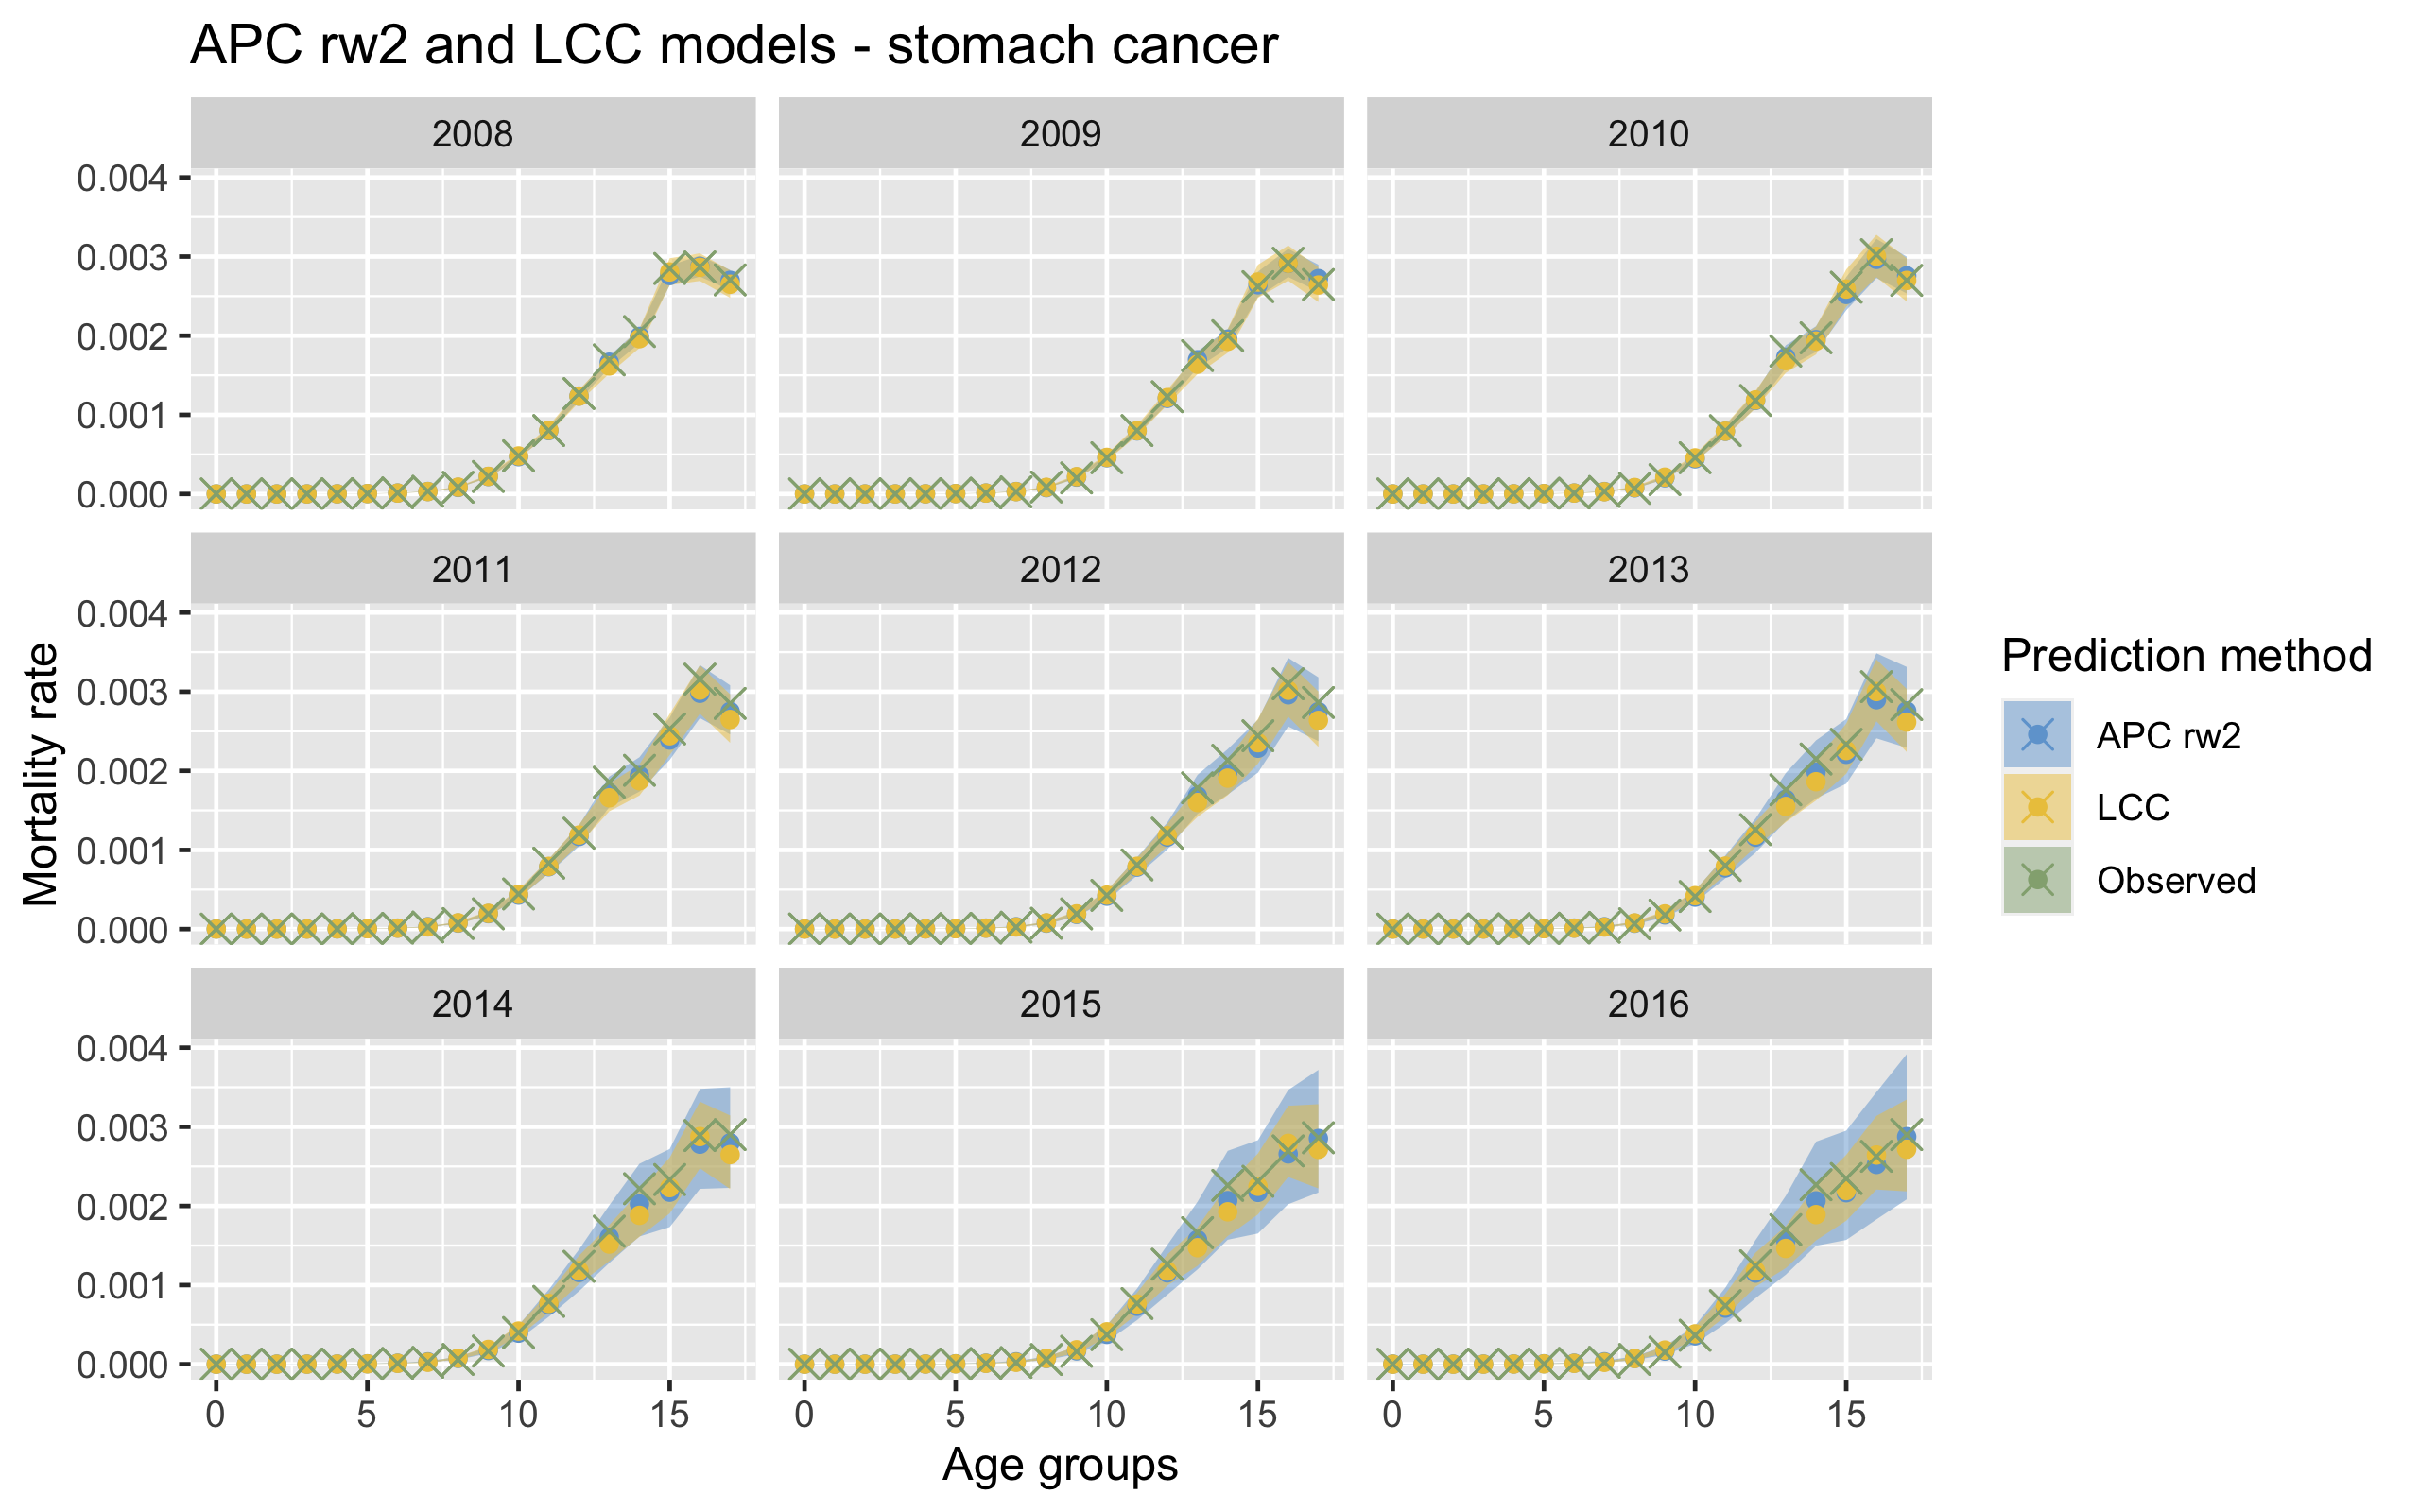
\includegraphics[width=\linewidth]{real-data/real-data-univariate/Figures/univariate-comparison-by-age-lung.png}
    \end{subfigure}
    \begin{subfigure}[b]{.45\linewidth}
        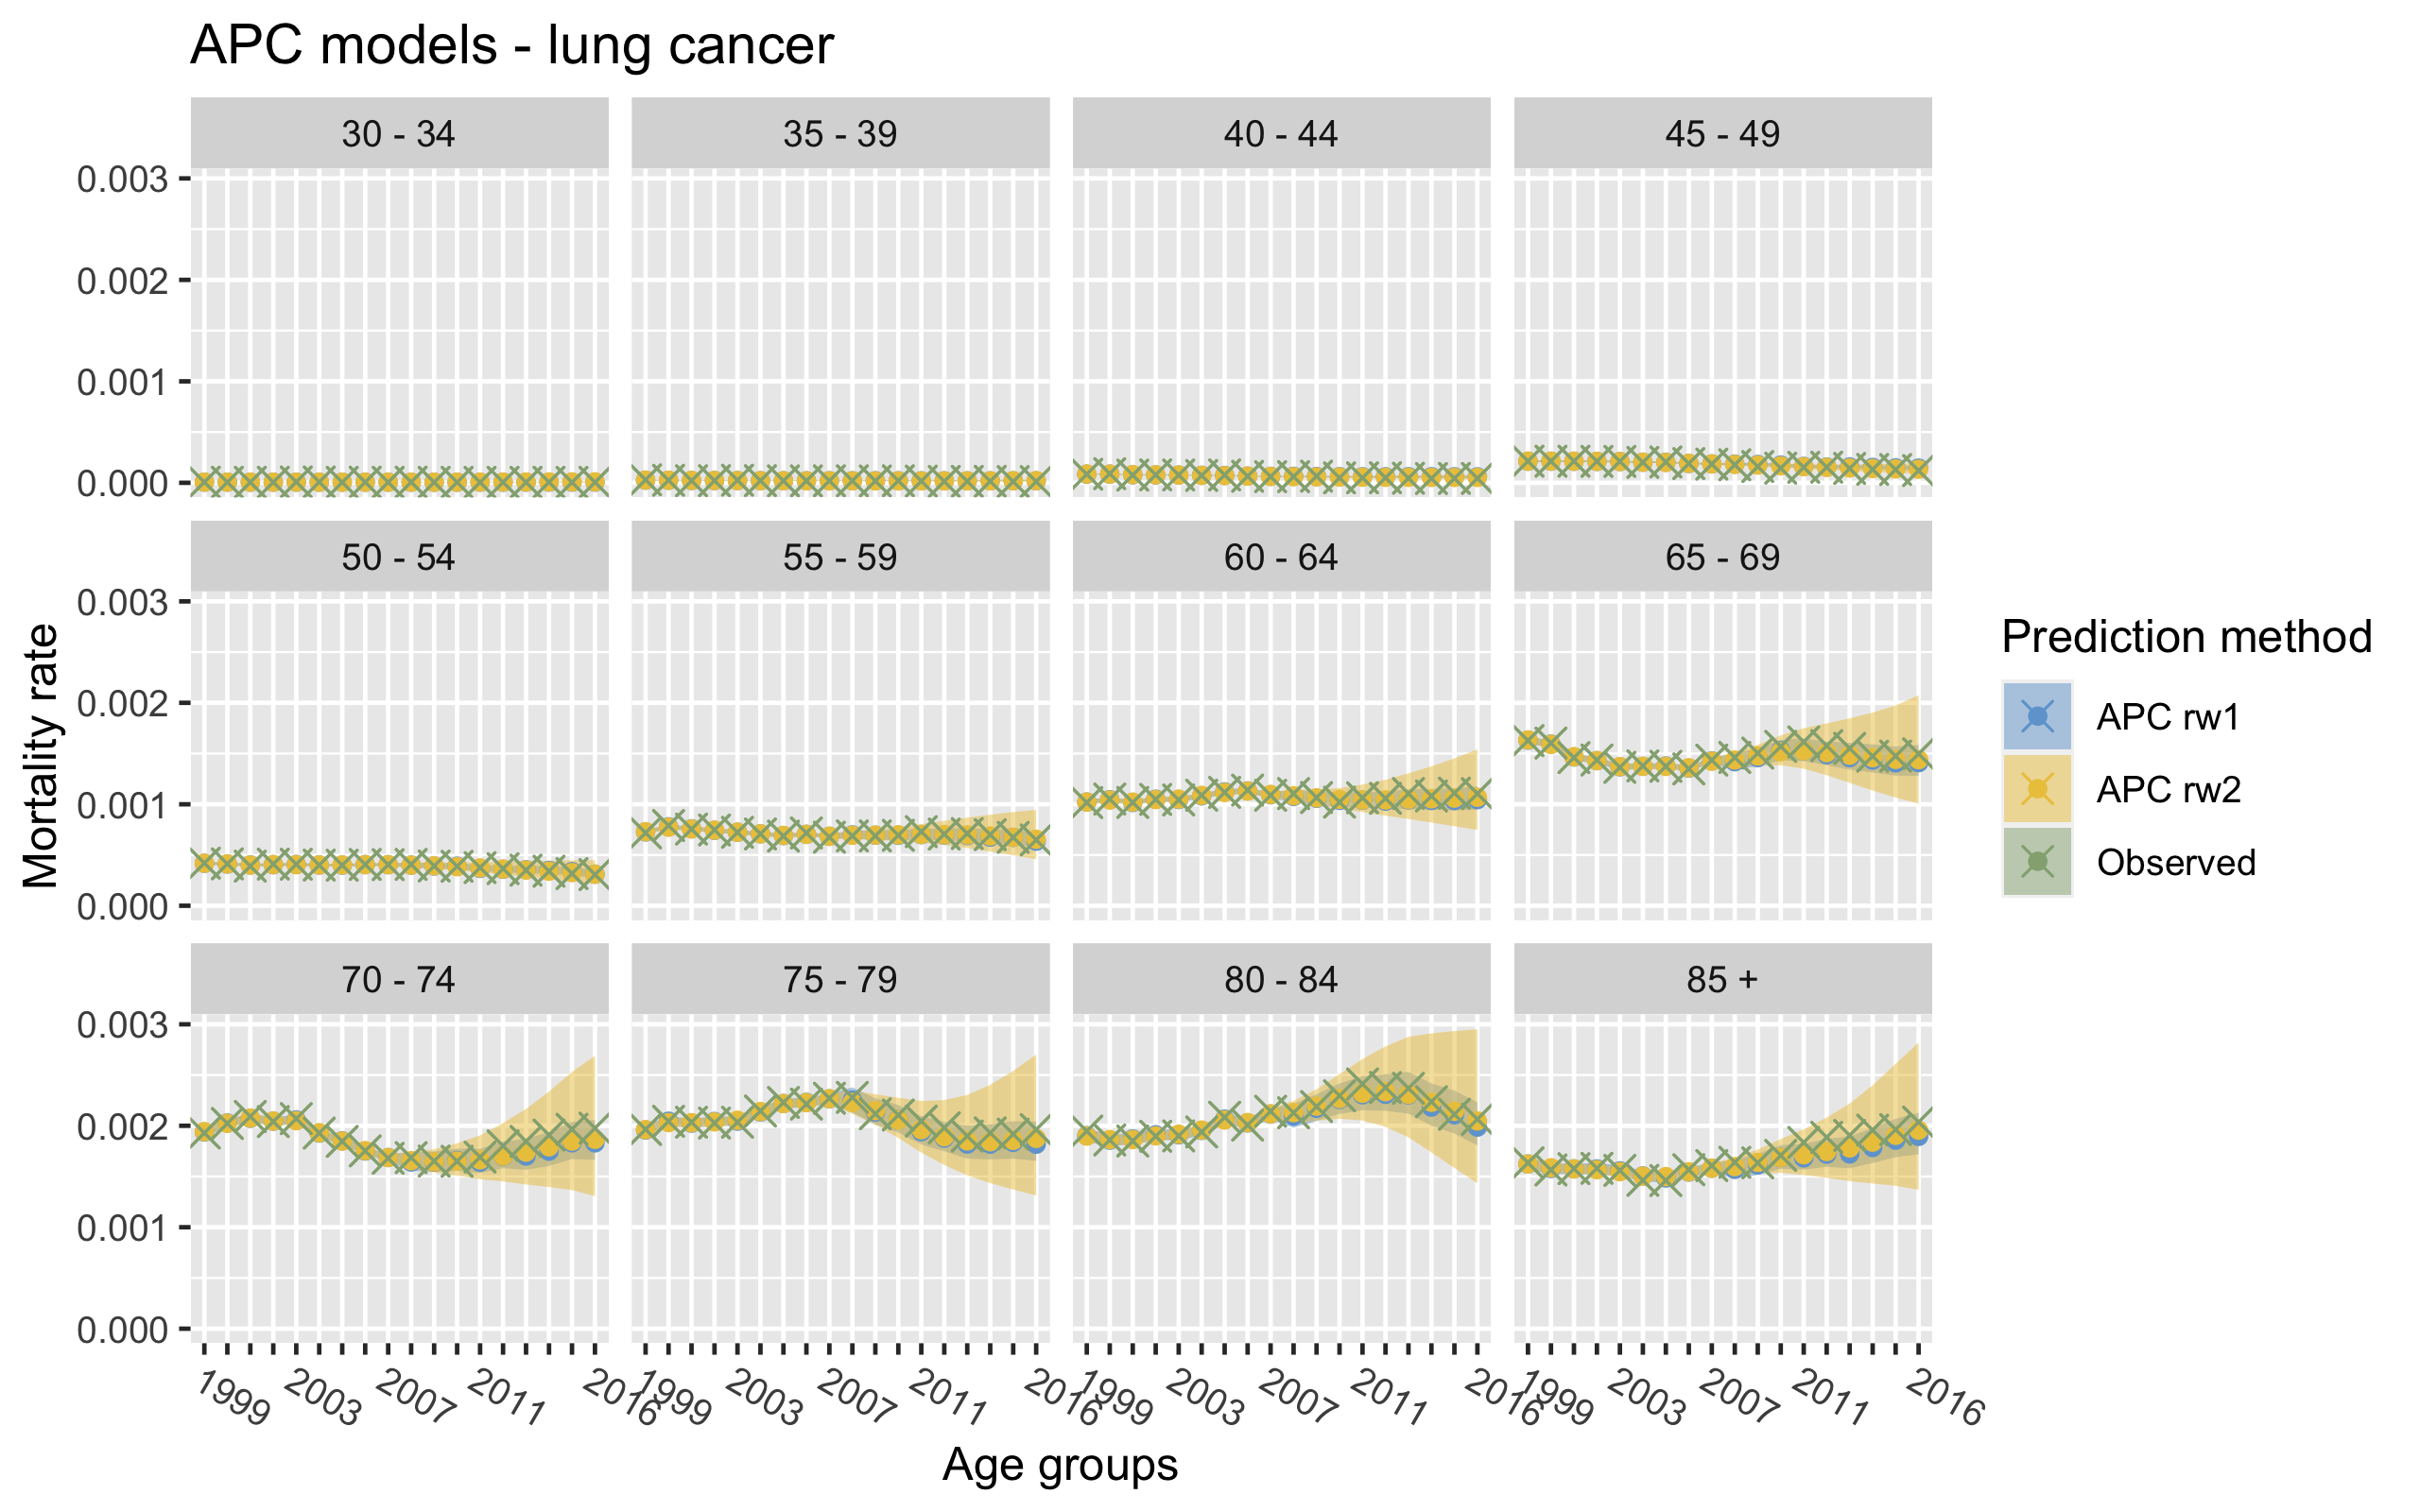
\includegraphics[width=\linewidth]{real-data/real-data-univariate/Figures/univariate-comparison-by-period-lung.png}
    \end{subfigure}
    \caption{The best-performing APC and LC-type models for lung cancer}
    \label{fig:uv-comparison-lung}
\end{figure}

\begin{figure}[h!]
    \centering
    \begin{subfigure}[b]{.45\linewidth}
        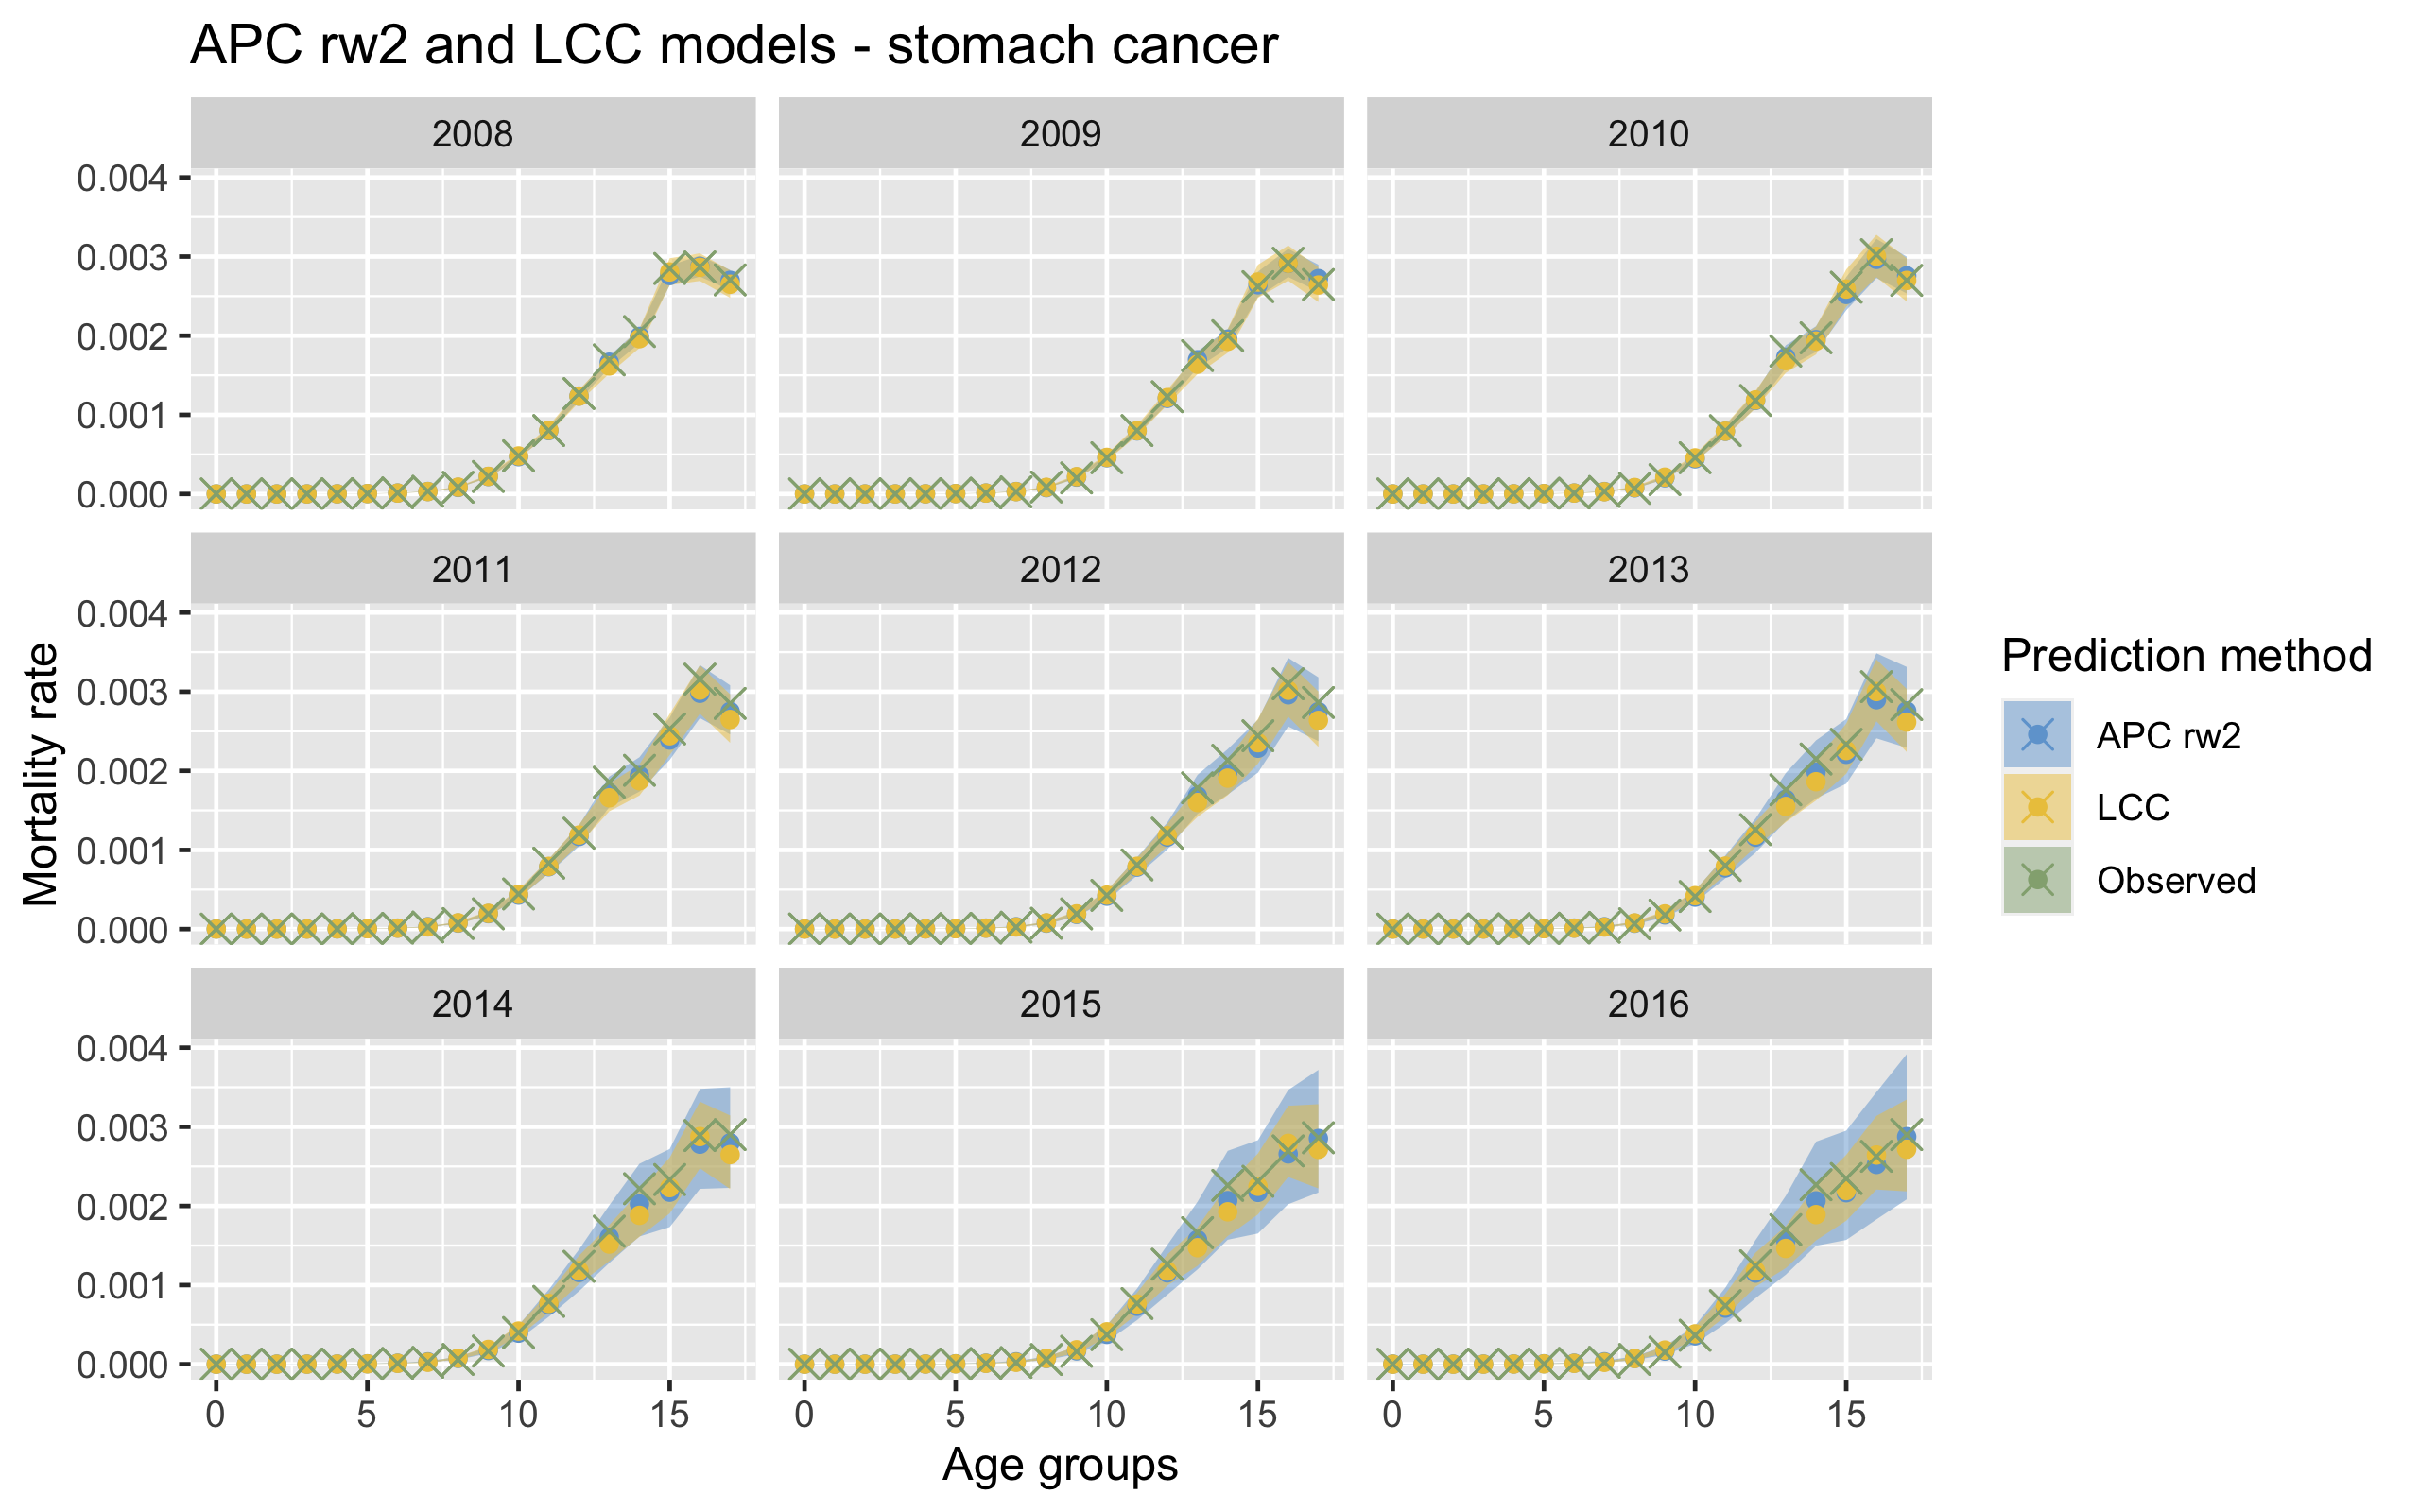
\includegraphics[width=\linewidth]{real-data/real-data-univariate/Figures/univariate-comparison-by-age-stomach.png}
    \end{subfigure}
    \begin{subfigure}[b]{.45\linewidth}
        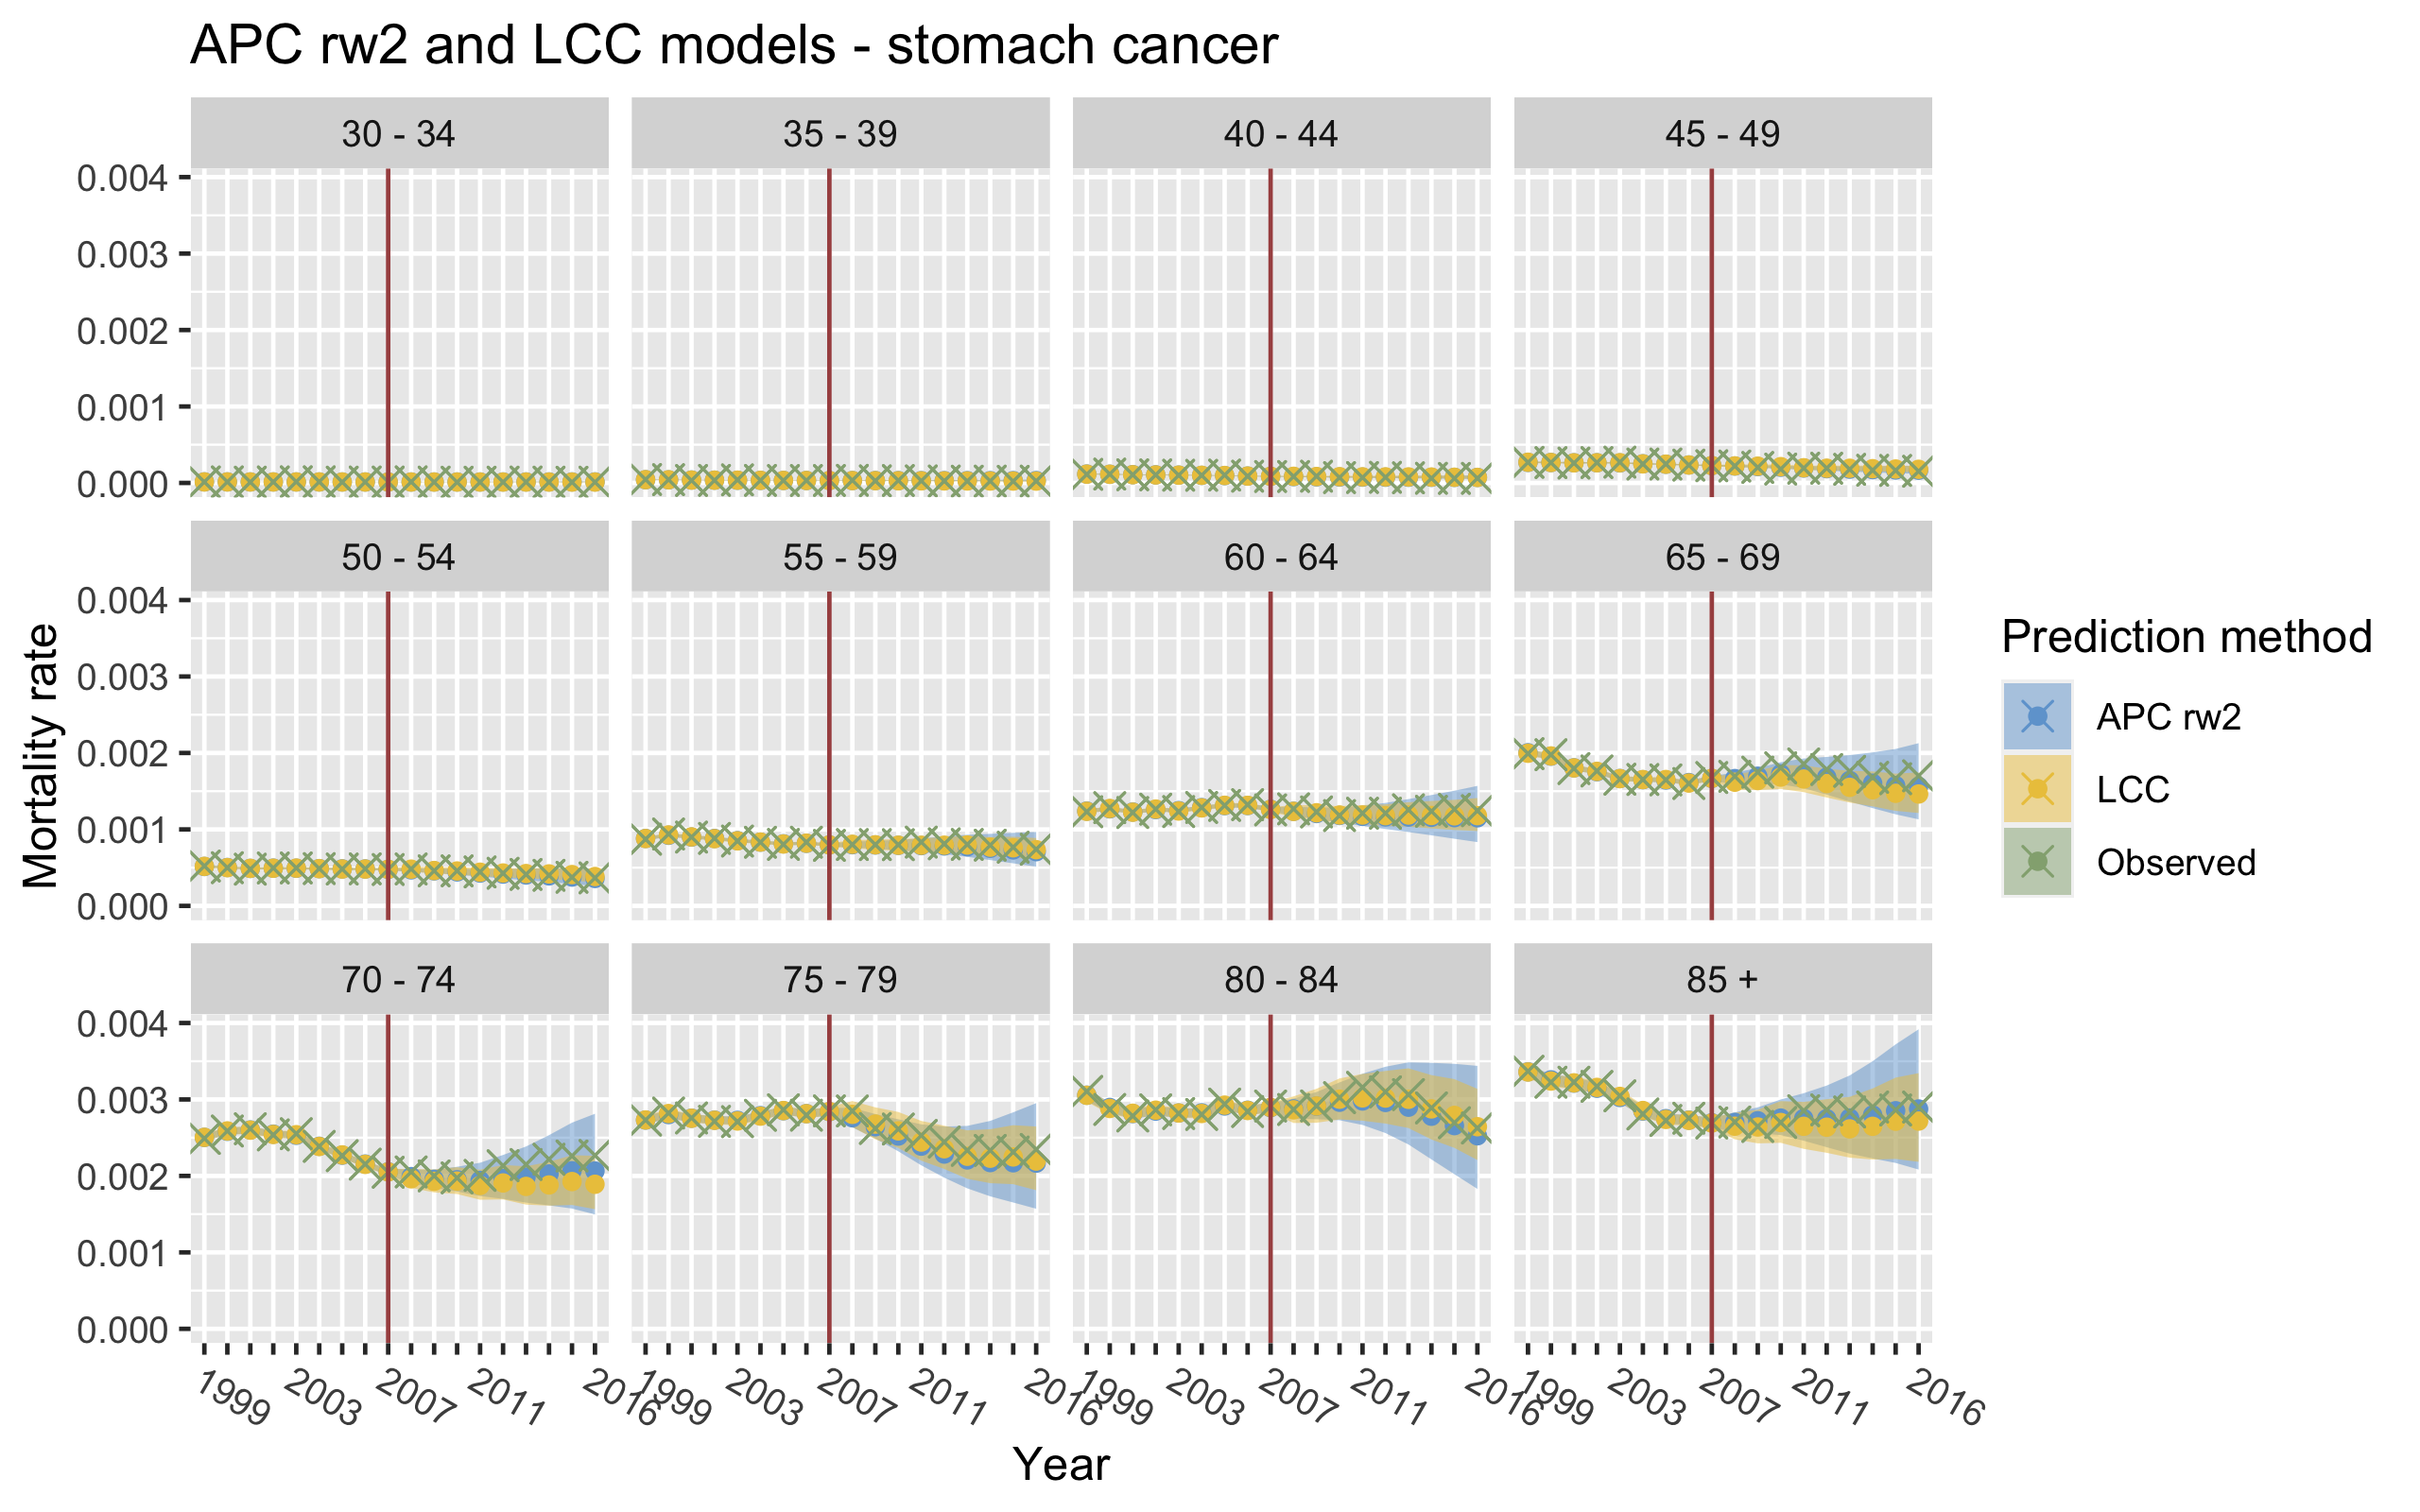
\includegraphics[width=\linewidth]{real-data/real-data-univariate/Figures/univariate-comparison-by-period-stomach.png}
    \end{subfigure}
    \caption{The best-performing APC and LC-type models for stomach cancer}
    \label{fig:uv-comparison-stomach}
\end{figure}

Figures \ref{fig:uv-comparison-lung} and \ref{fig:uv-comparison-stomach} display the results from the Lee-Carter and the APC models with the lowest MDSS, the LCC- and the APC2-models respectively. For both cancer types, the APC2-model has a lower MDSS than the LCC-model does (see Tables \ref{tbl:uv-lung-5} and \ref{tbl:uv-stomach-5}), and we see from the plotted results that the APC2-model seems to be slightly more accurate than the LCC-model. We do, however note that the prediction intervals are narrower for the LCC-model predictions for both cancer types.

\subsection{Sensitivity Analysis - choice of priors for $\alpha_x$ and $\gamma_k$}
\textcolor{myDarkBlue}{Not finished. Not sure if I should include it. }
\textcolor{myDarkGreen}{Include this section if time: show that your choice of random walk priors for kappa and alpha does not change the prediction results - in comparison with choosing AR1 gamma (as in \textcite{Wisniowski2015}) or iid alpha (as in \textcite{Wisniowski2015}). 
You have the code, you just need to tidy it. 
}

\newpage
\subsection{Prediction in the Multivariate Case}
\label{sec:pred-mv}

\textcolor{myDarkGreen}{
Intro: forskjell på multivariate og univariate. Referer til figuren av plottet data - tydelig forskjell på kjønnene, som kan tyde på at en multivariate modell vil fungere bedre. 
}

\textcolor{myDarkGreen}{Thought: For the multivariate version where all effects are kept common, you should also have a common intercept! If not it might be very different to adjust one random effect to two different overall mortality rates? Or, if this is difficult, should the male and female intercept just be the same? }

From the plots of the cancer mortality data in Section \ref{sec:GermanCancerData}, we observe a significant difference in male and female mortality rates, for both cancer types. The investigation of multivariate models with sex as a covariate, is then a natural next step in our analysis. We fit multivariate versions of Lee-Carter and APC models to the observed male and female cancer deaths, and use the male and female populations as the at-risk values. To avoid having to compare too many different models, we test only the Lee-Carter and APC models that displayed the best MDSS in the univariate case, namely the LCC-model and the APC2-model (for both lung and stomach cancer). We use the approach described in Section \ref{sec:multivariateAPC} to obtain multivariate versions of the LCC- and APC2-model, namely keeping some of the random effects common across the sexes. It is not clear from the plots of the data which, if any, of the effects that should be kept common for male and female populations. Therefore, we find predictions using models with all combinations of common and separate age, period and cohort effects, and compare the results. We test the following versions of the LCC-model:
\begin{itemize}
    \item All common: $\eta_{x,t,s} = \mu_s + \alpha_x + \beta_x(\phi\cdot t + \kappa_t) + \gamma_k + \epsilon_{x,t,s}$
    \item Common age, period: $\eta_{x,t,s} = \mu_s + \alpha_x + \beta_x(\phi\cdot t + \kappa_t) + \gamma_{k,s} + \epsilon_{x,t,s}$
    \item Common age, cohort: $\eta_{x,t,s} = \mu_s + \alpha_x + \beta_x(\phi_s\cdot t + \kappa_{t,s}) + \gamma_{k} + \epsilon_{x,t,s}$
    \item Common period, cohort: $\eta_{x,t,s} = \mu_s + \alpha_{x,s} + \beta_{x,s}(\phi\cdot t + \kappa_t) + \gamma_{k} + \epsilon_{x,t,s}$
    \item Common age: $\eta_{x,t,s} = \mu_s + \alpha_x + \beta_x(\phi_s\cdot t + \kappa_{t,s}) + \gamma_{k,s} + \epsilon_{x,t,s}$
    \item Common period: $\eta_{x,t,s} = \mu_s + \alpha_{x,s} + \beta_{x,s}(\phi\cdot t + \kappa_{t}) + \gamma_{k,s} + \epsilon_{x,t,s}$
    \item Common cohort: $\eta_{x,t,s} = \mu_s + \alpha_{x,s} + \beta_{x,s}(\phi_s\cdot t + \kappa_{t,s}) + \gamma_{k} + \epsilon_{x,t,s}$
    \item No common: $\eta_{x,t,s} = \mu_s + \alpha_{x,s} + \beta_{x,s}(\phi_s\cdot t + \kappa_{t,s}) + \gamma_{k,s} + \epsilon_{x,t,s}$
\end{itemize}
Note that the "No common" version of the model is equivalent to fitting two separate univariate LCC models to the male and female parts of the data. Note also that we always keep $\alpha_x$ and $\beta_x$ either common or separate, where we could have included all versions of the model where one is kept common and the other is separate. This is simply to reduce the number of models we need to compare, and because we do not expect it to have a lot of impact on the result. \textcolor{myDarkGreen}{Do you have enough reason to say this? }
For the APC2-model, we test the following multivariate versions:
\begin{itemize}
    \item APC: $\eta_{x,t,s}= \mu_{s} + \rho_x + \phi_t + \psi_k + \epsilon_{x,t,s}$ 
    \item APc: $\eta_{x,t,s}= \mu_{s} + \rho_x + \phi_t + \psi_{k,s} + \epsilon_{x,t,s}$ 
    \item ApC: $\eta_{x,t,s}= \mu_{s} + \rho_x + \phi_{t,s} + \psi_{k} + \epsilon_{x,t,s}$ 
    \item aPC: $\eta_{x,t,s}= \mu_{s} + \rho_{x,s} + \phi_{t} + \psi_{k} + \epsilon_{x,t,s}$ 
    \item aPc: $\eta_{x,t,s}= \mu_{s} + \rho_{x,s} + \phi_{t} + \psi_{k,s} + \epsilon_{x,t,s}$ 
    \item apC: $\eta_{x,t,s}= \mu_{s} + \rho_{x,s} + \phi_{t, s} + \psi_{k} + \epsilon_{x,t,s}$ 
    \item apc: $\eta_{x,t,s}= \mu_{s} + \rho_{x,s} + \phi_{t, s} + \psi_{k, s} + \epsilon_{x,t,s}$
\end{itemize}
Following \textcite{rieblerHeld2010}, we name the different versions of the APC2-model by capital letter for the common effects and shared letters for the male- and female-specific effects.  
\newpar To fit these multivariate models with \inlarbu, we need to alter the implementation of the prediction compared to the implementation of the univariate models. To implement the multivariate models, we use two likelihoods, one for each sex. For the effects that will not be common for male and females, we include two identical model components, named differently. These are included in one likelihood each. For the effects that are kept common, we only include one model component, which is used in both likelihoods. We only include male data in the male likelihood and female data in the female likelihood. Below, the part of the code used to produce predictions for the aPc-model is shown:

\begin{verbatim}
comp.aPc = ~ -1 + 
  mu(s, model = "iid", hyper = list(prec = list(fixed = TRUE,
    initial = log(0.001)))) +
  rho0(x, model = "rw2", values = unique(stomach.cancer$x), constr = TRUE,
    hyper = pc.prior, scale.model = TRUE) + 
  rho1(x, model = "rw2", values = unique(stomach.cancer$x), constr = TRUE,
    hyper = pc.prior, scale.model = TRUE) + 
  phi(t, model = "rw2", values = unique(stomach.cancer$t), constr = TRUE,
    hyper = pc.prior, scale.model = TRUE) + 
  psi0(k, model = "rw2", values = unique(stomach.cancer$k), constr = TRUE,
    hyper = pc.prior, scale.model = TRUE) + 
  psi1(k, model = "rw2", values = unique(stomach.cancer$k), constr = TRUE,
    hyper = pc.prior, scale.model = TRUE) + 
  epsilon(xts, model = "iid", hyper = pc.prior)

# define two different likelihoods and formulas, for male (0) and female (1):
form.aPc.0 = cases ~ -1 + mu + rho0 + phi + psi0 + epsilon
likelihood.aPc.0 = like(formula = form.aPc.0, family = "poisson",
    data = /*data frame containing male mortality cases*/,
    E = /*data frame containing male population*/)

form.aPc.1 = cases ~ -1 + mu + rho1 + phi + psi1 + epsilon
likelihood.aPc.1 = like(formula = form.aPc.1, family = "poisson",
    data = /*data frame containing female mortality cases*/,
    E = /*data frame containing female population*/)

res.aPc = bru(components = comp.aPc,
              likelihood.aPc.0,
              likelihood.aPc.1,
              options = list(/*Desired options*/
              )) 
\end{verbatim}
\newpar We perform the preciction analysis in the same way as for the univariate case, using the years 1999-2007 to fit the models and then predict the mortality for years 2008-2016. We use the same hyperpriors as for the univariate analysis, namely PC priors with parameters $\mathbb{P}(1/\sqrt{\tau} > 1) = 0.05$, and we gain exclude the predictions for ages younger than 30 years old ($x \leq 5$) when we calculate the score statistics.

We present the results for lung and stomach cancer, respectively, in the following two sections.

\import{}{Report/4-Real-data/mv-lung.tex}

\import{}{Report/4-Real-data/mv-stomach.tex}

\newpage
\subsection{Sensitivity analysis}

Throughout our analysis, we have used the same informative priors for all hyperparameters, for both the Lee-Carter models and the APC-models, without considering the effect this choice have on the prediction results. To investigate whether predictions with different hyperpriors would produce a different result, we run the analysis using the aPc-model with three different prior distributions and compare the results. \textcolor{myDarkGreen}{Sett inn tabell i stedet for Figure}. The score statistics for the different runs are presented in Table TODO. We observe that the predictions using the different hyperpriors have very similar score statistics, an indication that our choice of hyperpriors did not significantly influence the result. 

\begin{figure}[h!]
    \centering
    \begin{subfigure}[b]{.45\linewidth}
        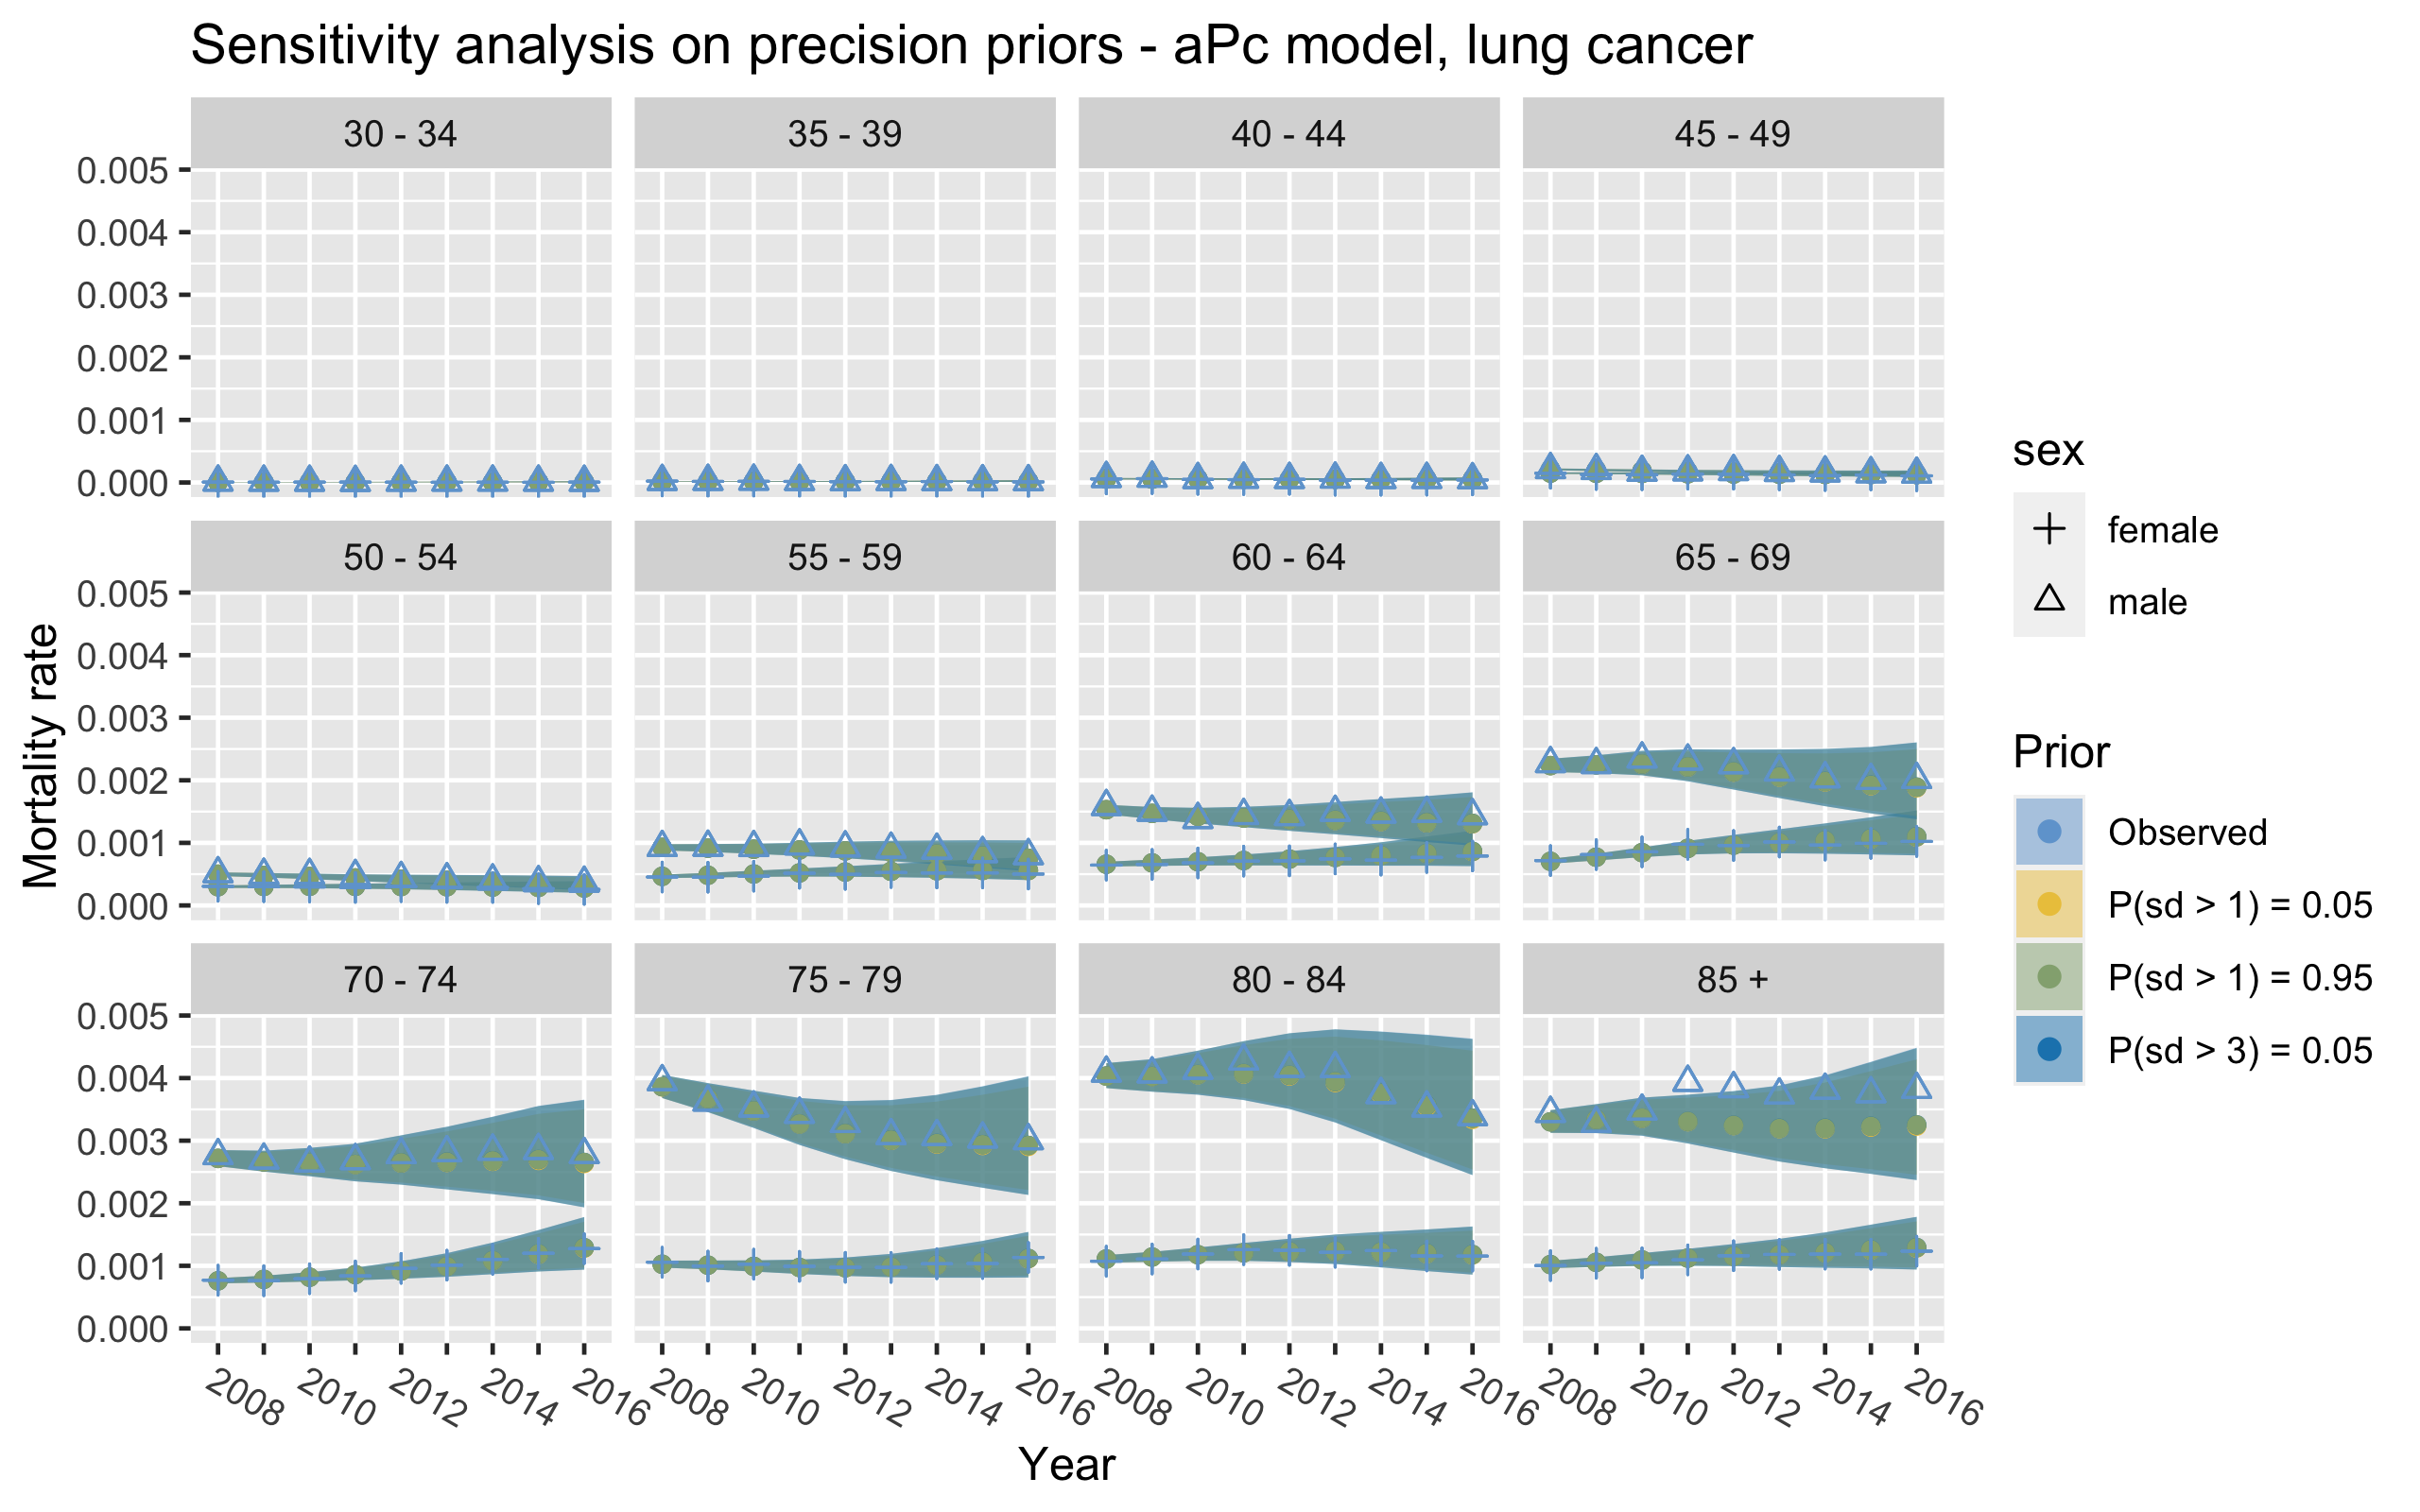
\includegraphics[width=\linewidth]{real-data/real-data-multivariate/Figures/sensitivity-analysis-aPc-by-period-lung.png}
    \end{subfigure}
    \begin{subfigure}[b]{.45\linewidth}
        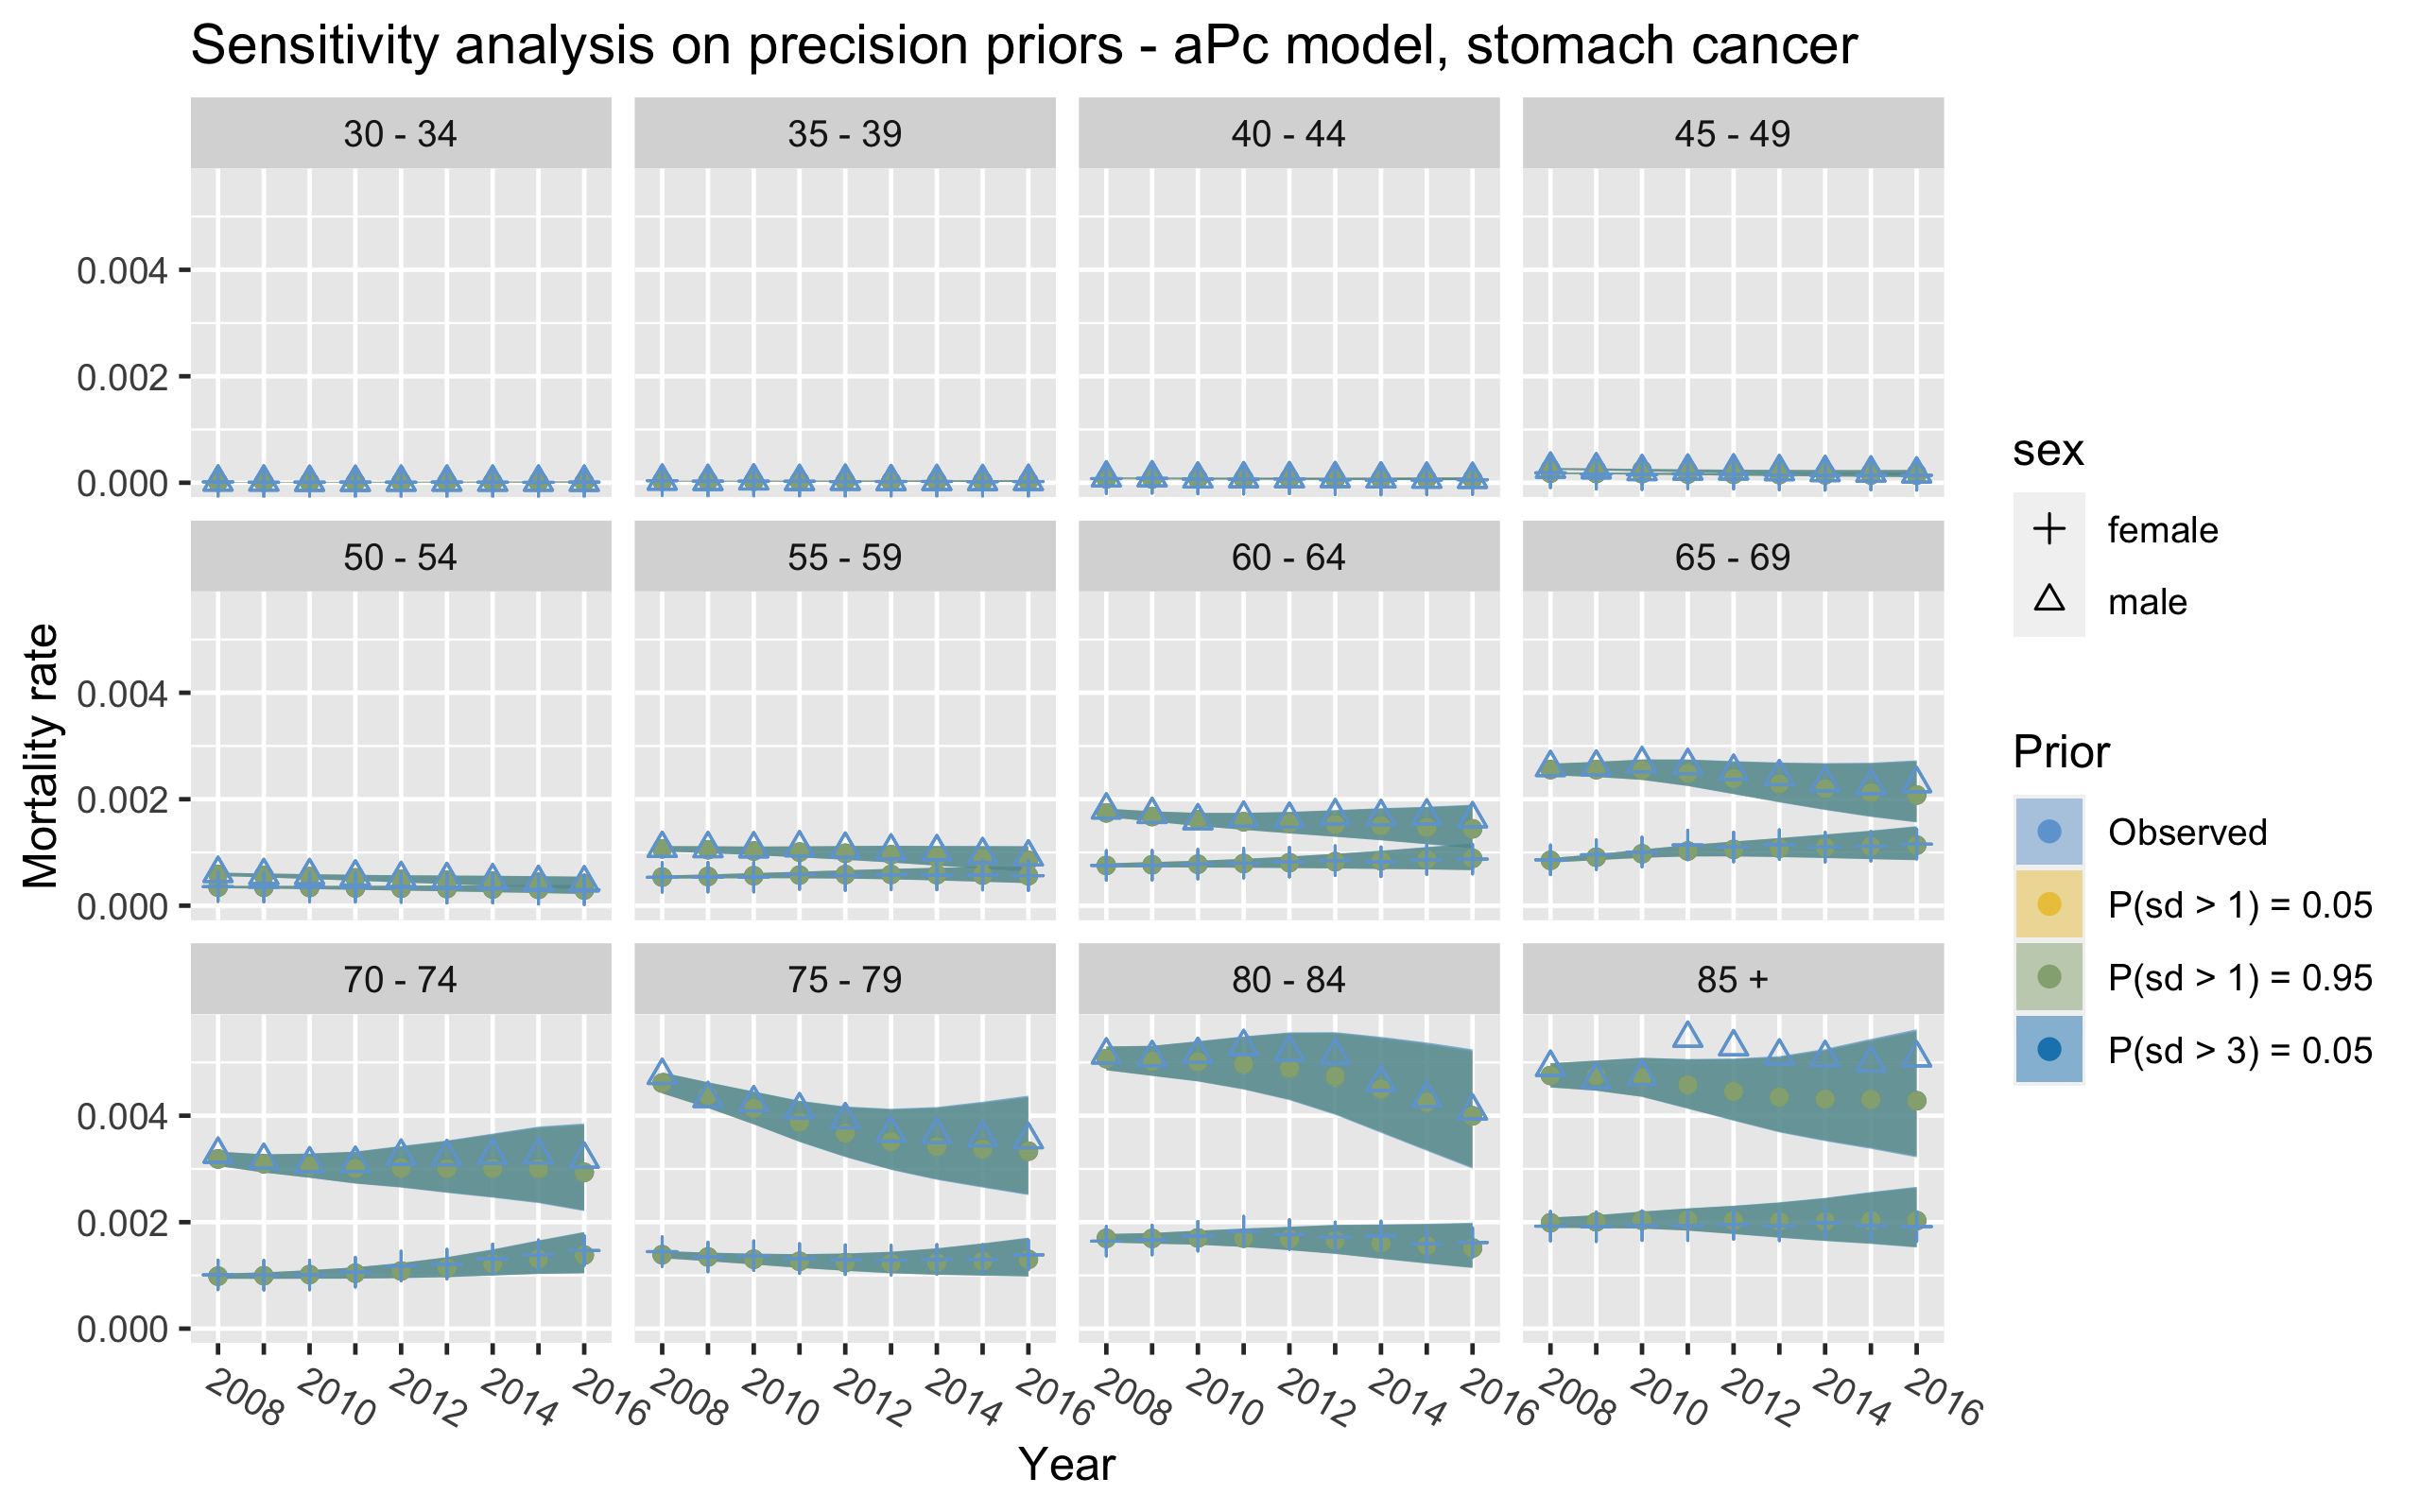
\includegraphics[width=\linewidth]{real-data/real-data-multivariate/Figures/sensitivity-analysis-aPc-by-period-stomach.png}
    \end{subfigure}
    \caption{Results from sensitivity analysis of the model that displayed the best predctive performance for lung cancer, the aPc-model (left), and stomach cancer, also the aPc model (right). \textcolor{myDarkGreen}{Remove this image if we have the table?}}
    \label{fig:mv-sensitivity}
\end{figure}

\newpage 
\subsection{Identifiability issues}
\textcolor{myDarkBlue}{This is not finished, but I don´t know if we still need to include a separate section about this? Or if we should move all the discussion about the effects of the plots here? }
\textcolor{myDarkGreen}{
Here, you can mention apparent identifiability issues. Perhaps talk about periodicity in cohort effects? Mention that a linear kappa might have been sufficient. 

\parencite{Wisniowski2015} states that the LCC model is identifiable as long as the betas are significantly different --> discuss if this is true in your case! (It does not seem like it is...)
}